\documentclass[12pt]{article}

% ============================================================
% Page layout and paragraph spacing
% ============================================================
\usepackage[letterpaper, top=1in, bottom=1in, left=1.05in, right=1.05in]{geometry}
\usepackage{setspace}
\setstretch{1.35}
\raggedbottom

% Float spacing
\setlength{\textfloatsep}{14pt plus 3pt minus 3pt}
\setlength{\floatsep}{12pt plus 3pt minus 3pt}
\setlength{\intextsep}{12pt plus 3pt minus 3pt}
\setlength{\abovecaptionskip}{6pt}
\setlength{\belowcaptionskip}{4pt}

\renewcommand{\topfraction}{0.90}
\renewcommand{\bottomfraction}{0.80}
\renewcommand{\textfraction}{0.08}
\renewcommand{\floatpagefraction}{0.75}
\setcounter{topnumber}{3}
\setcounter{bottomnumber}{2}
\setcounter{totalnumber}{5}

% ============================================================
% Mathematics
% ============================================================
\usepackage{amsmath,amssymb,amsfonts,bm,mathtools}

% ============================================================
% Tables
% ============================================================
\usepackage{array}
\usepackage{booktabs}
\usepackage{tabularx}
\usepackage{longtable}
\usepackage{multirow}
\usepackage{threeparttable}
\usepackage{adjustbox}

% ============================================================
% Figures, colors, and floats
% ============================================================
\usepackage{graphicx}
\usepackage{xcolor}
\usepackage{float}
\usepackage{placeins}
\usepackage{needspace}

\graphicspath{
  {./}
  {output/figures/main/}
  {output/figures/appendix/}
}

% ============================================================
% TikZ
% ============================================================
\usepackage{tikz}
\usetikzlibrary{
  arrows.meta,
  positioning,
  fit,
  calc,
  backgrounds,
  decorations.pathreplacing,
  shapes.geometric
}

% ============================================================
% Captions
% ============================================================
\usepackage{caption}
\usepackage{subcaption}

\captionsetup{
  font=small,
  labelfont=bf,
  labelsep=quad,
  justification=centering,
  singlelinecheck=true
}

\captionsetup[subfigure]{
  font=small,
  labelfont=bf,
  justification=centering,
  singlelinecheck=true
}

% ============================================================
% URLs, hyperlinks, and cross-references
% ============================================================
\usepackage{xurl}
\usepackage[
  hidelinks,
  unicode,
  bookmarksnumbered=true,
  bookmarksopen=true
]{hyperref}
\usepackage[nameinlink,noabbrev]{cleveref}

\crefname{figure}{Figure}{Figures}
\Crefname{figure}{Figure}{Figures}
\crefname{table}{Table}{Tables}
\Crefname{table}{Table}{Tables}
\crefname{equation}{Equation}{Equations}
\Crefname{equation}{Equation}{Equations}
\crefname{section}{Section}{Sections}
\Crefname{section}{Section}{Sections}
\crefname{subsection}{Section}{Sections}
\Crefname{subsection}{Section}{Sections}

\emergencystretch=2em

% Prevent common math commands from producing bookmark warnings.
\pdfstringdefDisableCommands{%
  \def\bm#1{#1}%
  \def\mathrm#1{#1}%
  \def\textnormal#1{#1}%
  \def\textit#1{#1}%
  \def\text#1{#1}%
  \def\top{}%
}

% ============================================================
% Section formatting
% ============================================================
\usepackage{titlesec}
\titleformat{\section}{\Large\bfseries}{\thesection}{1em}{}
\titleformat{\subsection}{\large\bfseries}{\thesubsection}{1em}{}
\titleformat{\subsubsection}{\normalsize\bfseries}{\thesubsubsection}{1em}{}

% ============================================================
% Bibliography
% ============================================================
\renewcommand{\refname}{References}

% ============================================================
% Long AP-Tree node names
% ============================================================
\let\APTreeOriginalUnderscore\_
\newcommand{\APTreeBreakableUnderscore}{%
  \APTreeOriginalUnderscore\allowbreak
}

% ============================================================
% Common abbreviations
% ============================================================
\newcommand{\APT}{\textnormal{AP-Tree}}
\newcommand{\TS}{\textnormal{TripleSort64}}
\newcommand{\DeepBoost}{\textnormal{Deep Boost}}
\newcommand{\ShallowTilt}{\textnormal{Shallow Tilt}}
\newcommand{\SR}{\mathrm{SR}}
\newcommand{\XSRtwo}{\mathrm{XS}\text{-}R^{2}}

% ============================================================
% Document metadata
% ============================================================
\title{Depth-Weighted Selection in AP Trees: Local Information and Conditional Return Reversal in China}
\author{
Yuqi Mao\thanks{
Zhejiang University International Business School (ZIBS), Zhejiang University.
Email: \texttt{myq1401895664@163.com}.
}
\and
Guoliang Ma\thanks{
Corresponding author. , Xiamen University.
Email: \texttt{glma@xmu.edu.cn}.
}
}
\date{}

\begin{document}

\maketitle

\begin{abstract}

We introduce depth-weighted selection into AP-Trees, making node depth an explicit design dimension in sparse SDF construction. 
Deep Boost raises deeper nodes’ relative scale during selection without magnifying their final returns, allowing local information to compete with shallow nodes’ diversification advantage. 
Its advantage is strongest under tight support constraints: shallow weighting can oversmooth local signals, whereas larger supports narrow this difference but admit noisy assets and increase overfitting risk. 
After excluding the smallest $30\%$ of Chinese stocks and re-estimating the full pipeline, 
depth-weighted AP-Trees reveal conditional short-term reversal among relatively small stocks. Long- and short-side evidence indicates state-dependent price correction.

\end{abstract}

\noindent\textbf{Keywords:} AP-Tree, depth weighting, sparse stochastic discount factor, Chinese stock market, short-term reversal, shell value

\vspace{1em}
%\tableofcontents
\clearpage

\section{Introduction}

The central task of asset pricing is to identify common risk factors that drive cross-sectional differences in stock returns and to construct factor models that effectively explain these differences. Since Fama and French (1993) proposed the three-factor model, sorting-based factor construction has become the dominant empirical paradigm. This method sorts stocks by firm characteristics and constructs factor returns as the difference in returns between portfolios \cite{ref3}. Sorting is transparent and economically intuitive, but its results typically depend on the researcher's pre-specified characteristics, breakpoints, and ordering. Univariate sorting cannot capture interactions among firm characteristics; multivariate independent sorting produces finer intersection cells but still relies on fixed unconditional grids, thereby failing to identify nonlinear pricing relations that hold only in specific local states. As the ``factor zoo'' expands, extracting low-dimensional, robust, and economically interpretable pricing structures from a large set of characteristics and their interactions has become a major challenge.

Bryzgalova, Pelger, and Zhu (2025) introduce the AP-Tree method in \textit{The Journal of Finance} \cite{ref3}. AP-Tree generates managed portfolios with varying depths and local coverage through recursive conditional partitioning, and then selects a sparse set of basis assets that improve the mean-variance spanning of the stochastic discount factor (SDF) using the joint mean and covariance structure of all candidate nodes. Unlike conventional regression trees that split based on a single node's prediction error, AP-Tree does not directly predict individual stock returns; rather, it constructs a cross-section of tradable assets that span the conditional SDF. Compared with fixed sorting, AP-Tree allows breakpoints to vary with prior split paths, retains the root, intermediate, and terminal nodes simultaneously, and endogenously chooses between broadly diversified portfolios and deep nodes that capture local interactions. The method achieves high out-of-sample Sharpe ratios and strong pricing power in the U.S. equity market, but its applicability to the Chinese A-share market—where institutional background, investor structure, and trading mechanisms differ substantially—remains to be tested empirically.

The Chinese A-share market provides a discriminating environment for testing the cross-market validity of AP-Tree. On the one hand, the A-share market has high retail participation, making stock returns more susceptible to investor sentiment, short-term trading, liquidity shocks, and policy expectations. Leippold, Wang, and Zhou (2022) apply various machine learning methods to Chinese stock returns and find that liquidity is an important predictor, and that retail-trading-related characteristics have strong predictive power for short-term returns of small-cap stocks \cite{ref15}. This suggests that pricing information in the Chinese market may concentrate more on nonlinear interactions among size, trading activity, and recent price states, rather than on relatively stable linear factor exposures found in developed markets.

On the other hand, the Chinese stock market has institutional sample issues that general machine learning frameworks cannot ignore. Liu, Stambaugh, and Yuan (2019) show that the lowest market-capitalization stocks in the A-share market may contain significant shell value due to the backdoor listing mechanism, distorting the empirical performance of traditional size and value factors \cite{ref17}. If a high-dimensional model can flexibly choose local stock portfolios from a larger candidate space, it may also concentrate more heavily on micro-cap stocks with special institutional premiums. This raises an important identification problem: does a high out-of-sample Sharpe ratio mean the model discovers a generalizable conditional pricing structure, or does it merely repackage the shell-value returns of the smallest stocks in a more complex way? Therefore, testing AP-Tree in the Chinese market cannot simply compare performance metrics in the raw sample; it must also examine whether model weights concentrate in the potential shell-value region, and re-construct all candidate assets and the SDF after excluding that region.

Li, Liu, Liu, and Wei (2024) systematically replicate anomalies in the Chinese A-share market and find that many anomalies originating from the U.S. market do not hold robustly in China, emphasizing that factor tests must fully account for the sample structure and local factor models \cite{ref16}. This evidence further suggests that the flexibility of machine learning models does not automatically imply cross-market robustness. Even if a model identifies complex relations in a given sample, it may merely amplify the returns of a particular period or stock group. Hence, evaluating AP-Tree requires simultaneous examination of fully out-of-sample returns, whether existing factors explain the final portfolio, whether they explain the underlying node assets, and whether the portfolio remains stable after excluding special stock groups.

In recent years, machine learning applications in Chinese asset pricing have deepened. Zhu (2025) employs deep neural networks to construct deep factors based on various firm characteristics—value, intangibles, investment, profitability, frictions, and momentum—and finds that momentum, value, and frictions are overall important, but their relative roles vary across portfolios \cite{ref22}. Ni et al. (2022) generate portfolio asset spaces via binary trees using value, size, and turnover, and find that high-dimensional asset spaces formed by tree nodes improve out-of-sample portfolio performance \cite{ref19}. These studies indicate that nonlinear models may capture local characteristic interactions in the Chinese market, but they do not systematically answer three interrelated questions: first, whether AP-Tree's performance in China depends on micro-caps and shell value; second, what pricing information is contained in deep local nodes versus shallow diversified nodes; and third, which specific conditional paths drive the model's high returns and whether these paths can be explained by major Chinese and international factor models.

This paper addresses these questions by systematically applying AP-Tree to the Chinese A-share market. Based on size and nine additional firm characteristics, we construct 36 three-characteristic cross-sections and compare AP-Tree with TripleSort64 under the same characteristic information. TripleSort64 uses fixed unconditional quartile grids to form cross portfolios; AP-Tree generates overlapping nodes of varying depths via conditional splits within parent nodes and selects nodes based on their incremental contributions to SDF spanning under a sparse penalty. We strictly follow chronological splits into training, validation, and fully out-of-sample test periods, with January 2021–December 2025 as the final test sample. To identify the influence of micro-caps and potential shell value, we further exclude the lowest $30\%$ of stocks by market capitalization each month, and re-determine breakpoints, generate candidate assets, select hyperparameters, and estimate the SDF in the cleaned universe. Thus, the cleaned-sample test re-identifies the pricing structure after excluding the potential shell-value region, rather than ex post truncating original portfolio returns.

Our core methodological extension treats node depth weighting as an economically meaningful selection dimension rather than a mere algorithmic parameter. Let node \(i\) cover \(N_i\) stocks in a given month. The original diversification adjustment of Bryzgalova, Pelger, and Zhu (2025) scales candidate nodes by \(\sqrt{N_i}\) before they enter the sparse selection path, giving higher relative scale to shallower, larger-coverage nodes. We call this Shallow Tilt. For an approximately balanced binary tree, since \(N_i\propto 2^{-d_i}\), where \(d_i\) is node depth, this transformation is equivalent to scaling nodes by \(2^{-d_i/2}\).

However, expanding node coverage does not necessarily eliminate all common fluctuations in the Chinese market. Policy shocks, correlated retail trading, investor sentiment, and industry co-movements may still impart strong systematic components to shallow portfolios. Meanwhile, the truly incremental cross-sectional pricing differences may concentrate in local regions jointly determined by size, recent price states, and trading frictions. For such state-dependent return differentials, only after successive conditional splits do the relevant stock groups separate from broader common components. Therefore, mechanically raising the relative scale of shallow nodes via \(\sqrt{N_i}\) may, while reducing firm-specific noise, oversmooth effective local signals and prevent them from entering the sparse support set. To test this possibility, we construct the mirror transformation \(\sqrt{1/N_i}\), which raises the relative scale of small-coverage, deep nodes, and call it Deep Boost. In an approximately balanced tree, this corresponds to \(2^{d_i/2}\). The two transformations differ only in the relative scale before sparse selection; after node selection and parameter estimation, we rescale coefficients back to the original node-return scale to construct the final SDF. Thus, Deep Boost does not mechanically amplify the final returns of deep nodes, but alters the model's selection boundary between shallow diversification and deep local information under a given complexity constraint.

Node depth weighting and support set size play distinct, non-substitutable roles: the former determines which type of information is prioritized in the sparse support set, while the latter controls the trade-off between information coverage and estimation error. We compare the two transformations under \(K_{\max}=20\) and \(K_{\max}=40\). If effective pricing information resides mainly in broadly covered, diversified portfolios, Shallow Tilt should perform better out-of-sample; if incremental information concentrates in local groups identified by successive conditional splits, Deep Boost should be more advantageous when the support set is small and sparse constraints are tight, and should select nodes that are harder to span by existing linear factors. Expanding the support set may narrow the gap between the two transformations, but it also increases the risk of fitting in-sample noise and thus cannot substitute for depth weighting.

We obtain three main findings. First, AP-Tree does not replicate its overwhelming advantage over traditional sorting in the U.S. market when applied to the raw Chinese sample. In the full universe, the best-performing SDFs come from both AP-Tree and TripleSort64, and the main positive weights of both types are heavily concentrated in the lowest \(30\%\) market-cap stocks, indicating that the high Sharpe ratios in the raw sample contain a significant micro-cap and shell-value component. After monthly exclusion of this region and re-determining breakpoints, generating candidate assets, and estimating the SDF, TripleSort64's out-of-sample performance declines more markedly, while AP-Tree exhibits greater robustness. In the cleaned sample, the six SDFs with the highest out-of-sample monthly Sharpe ratios all come from AP-Tree, with monthly Sharpe ratios between 0.613 and 0.721, and all retain significant positive \(\alpha\) under the CH3, CH4, FF5, FF6, Carhart4, and Q5 factor models. Thus, AP-Tree's relative advantage does not arise from complex repackaging of the lowest-cap stocks, but becomes evident only after removing shell-value contamination.

Second, the pricing value of deep nodes depends on the match between local signals and the sparse selection rule. When \(K_{\max}=20\), Deep Boost achieves a higher out-of-sample monthly Sharpe ratio in 23 of the 36 characteristic cross-sections and a higher average monthly excess return in 26 cross-sections, indicating that diversification-adjustment favoring broad-coverage nodes may exclude some local signals from the limited support set. When \(K_{\max}\) is increased to 40, the performance gap between the two depth weightings narrows overall, but adding nodes does not produce monotonic out-of-sample improvement, nor does it substitute for the choice of depth weighting. A larger support set, on the one hand, allows both specifications to cover a more similar node space; on the other hand, it increases the scope for fitting in-sample noise and fortuitous covariance structures. The most discriminating evidence comes from the \((\mathrm{LME},\mathrm{ST\_Rev},r_{12,2})\) cross-section: under \(K_{\max}=20\), Deep Boost raises the out-of-sample monthly Sharpe ratio from 0.613 to 0.703, and the selected nodes have negative XS-\(R^2\) under all six benchmark factor models. The incremental value of deep nodes thus does not stem from higher model complexity per se, but from preserving local assets that existing linear factors cannot span, subject to a constrained complexity budget.

Third, the high-Sharpe SDFs in the cleaned sample reveal a stable conditional short-term reversal within relatively small stocks. All 18 AP-Tree specifications with out-of-sample monthly Sharpe ratios exceeding 0.55 include both size and short-term reversal, and display a consistent direction across different third characteristics, depth weightings, and support-set sizes: buying relatively small-cap stocks that have recently underperformed and selling those that have recently risen. Since all portfolios are re-constructed after monthly exclusion of the lowest \(30\%\) of market-cap stocks, this return structure cannot be explained by extreme micro-caps or potential shell value. Medium-term momentum, long-term reversal, idiosyncratic volatility, and fundamental characteristics further determine the local states in which short-term reversal appears; the idiosyncratic volatility–momentum cross-section exhibits the strongest out-of-sample performance. These results indicate that short-term price correction in the Chinese market is significantly state-dependent, concentrating among relatively small stocks with higher arbitrage risk, and that unconditional cross-sorting averages out this local heterogeneity.

This paper makes three main contributions. First, we provide a systematic out-of-sample test of AP-Tree in the Chinese A-share market, placing its external validity in the context of China's specific micro-cap and shell-value environment. Rather than ex post deleting the smallest stocks from existing portfolios, we re-execute breakpoint determination, candidate asset generation, model selection, and SDF estimation separately in the full and cleaned universes. This design allows us to distinguish conditional pricing information identified by AP-Tree from institutional returns associated with the stock universe, and shows that cross-market comparisons of machine-learning asset-pricing methods must simultaneously consider market institutions and sample definitions.

Second, we treat node depth as an economically meaningful selection dimension rather than a mere algorithmic parameter. Shallow Tilt emphasizes the diversification role of broad-coverage nodes, while Deep Boost raises the relative chance of local nodes entering the limited support set. The paired design across different \(K_{\max}\) separates the choice of node scale from the choice of support-set size: the former determines whether the model prioritizes broad common components or local interactions, while the latter controls the trade-off among information coverage, estimation error, and in-sample fit. This framework thus provides a method for testing how pricing information is distributed along tree depth, rather than mechanically equating more nodes or deeper splits with a better model.

Third, we establish a complete attribution framework from statistical performance to economic mechanism. Out-of-sample Sharpe ratios and factor-adjusted \(\alpha\) measure whether the strategy generates incremental returns; node-level XS-\(R^2\) tests whether these returns can be spanned by existing factors in the cross-section; node paths locate the specific characteristic regions where returns arise. Combining these three types of evidence distinguishes effective repackaging of common factor exposures from truly local pricing errors, and reduces machine-learning-generated SDFs to interpretable, testable portfolio mechanisms. This approach also provides an empirical path for other high-dimensional asset-pricing models to move from predictive power to economic identification.

Overall, AP-Tree's main value in the Chinese market is not mechanically increasing candidate portfolios, node counts, or split depth, but rather identifying local pricing structures that fixed sorting misses after controlling for micro-cap contamination and model complexity. Our evidence locates this structure as a conditional short-term reversal within relatively small-cap stocks, modulated by historical price paths and arbitrage risk. Node depth weighting determines whether these local signals enter the limited support set, while support-set size determines the trade-off between information coverage and estimation error; the two are related but non-substitutable. This conclusion both explains why AP-Tree outperforms traditional sorting in the cleaned sample and delineates the economic conditions under which its advantage holds.

\clearpage

\section{Model and Methodology}
\label{sec:method}

This paper employs Asset Pricing Trees (AP-Tree) to construct managed portfolios that capture nonlinear relations and interactions among firm characteristics. AP-Tree first performs conditional recursive partitioning within a given characteristic cross-section, generating overlapping parent and child nodes; then, with the objective of mean-variance spanning of the stochastic discount factor (SDF), it selects a sparse set of basis assets from the candidate nodes \cite{ref3}. Unlike conventional regression trees that split based on a single node's return differential, AP-Tree evaluates a node's marginal pricing contribution from the joint mean and covariance structure of all candidate assets, and thus belongs to the class of global asset selection methods.

To adapt to the Chinese stock market, we construct candidate assets separately in the full universe and in a cleaned universe obtained by monthly exclusion of the lowest \(30\%\) of stocks by market capitalization, to identify the impact of micro-caps and shell value. Each characteristic cross-section always includes the size variable and selects two other variables from the remaining set, forming 36 three-characteristic cross-sections. We further compare two depth weightings—one favoring deep local nodes and the other favoring shallow diversified nodes—to examine the trade-off between local interaction information and portfolio diversification. Model selection uses only the development period; the 2021–2025 data are reserved as a fully out-of-sample test period.

For notational uniformity, scalars are denoted by ordinary italics, vectors by bold lowercase, matrices by bold uppercase, and sets by calligraphic letters. Superscript \(e\) denotes excess returns, superscript \(\top\) denotes transpose, and \(\bm 1_P\) and \(\bm I_P\) denote the \(P\)-vector of ones and the \(P\times P\) identity matrix, respectively.

\subsection{Conditional SDF, Managed Portfolios, and Test Asset Spanning}
\label{subsec:sdf_spanning}

Let \(R_{i,t}\) be the return of stock \(i\) in month \(t\), \(R_{f,t}\) the risk-free rate, and the excess return of stock \(i\) be
\begin{equation}
  R_{i,t}^{e}=R_{i,t}-R_{f,t}.
  \label{eq:stock_excess_return}
\end{equation}
Let \(N_t\) be the number of stocks in month \(t\), \(\bm c_{i,t-1}\in\mathbb R^M\) the \(M\)-dimensional firm characteristic vector known at portfolio formation, and \(\mathbb E_{t-1}(\cdot)\) the conditional expectation given the information set at \(t-1\). Conditional on firm characteristics, the projection of the minimum-variance SDF onto the space of stock returns can be written as
\begin{equation}
  \begin{aligned}
  M_t^{C}
  =1-\sum_{i=1}^{N_t} b_{i,t-1}
  \bigl[
    R_{i,t}^{e}
    -\mathbb E_{t-1}(R_{i,t}^{e})
  \bigr],
  \qquad
  b_{i,t-1}=f(\bm c_{i,t-1}),
  \end{aligned}
  \label{eq:conditional_sdf}
\end{equation}
where \(M_t^{C}\) is the conditional SDF, \(b_{i,t-1}\) is the conditional SDF loading of stock \(i\), and \(f:\mathbb R^M\rightarrow\mathbb R\) can be nonlinear, non-additive, and non-separable.

Approximate \(f(\cdot)\) by \(J\) basis functions \(\{f_j(\cdot)\}_{j=1}^{J}\):
\begin{equation}
  f(\bm c_{i,t-1})
  \approx
  \sum_{j=1}^{J}\omega_j f_j(\bm c_{i,t-1}),
  \label{eq:basis_approximation}
\end{equation}
where \(\omega_j\) is the coefficient for the \(j\)-th basis function. The managed portfolio excess return corresponding to the \(j\)-th basis function is defined as
\begin{equation}
  R_{j,t}^{\mathrm{man},e}
  =
  \sum_{i=1}^{N_t}
  f_j(\bm c_{i,t-1})R_{i,t}^{e}.
  \label{eq:managed_return_general}
\end{equation}
Consequently, the conditional asset pricing problem can be approximately transformed into an unconditional one using managed portfolios:
\begin{equation}
  M_t^{C}
  \approx
  1-\sum_{j=1}^{J}\omega_j
  \bigl[
    R_{j,t}^{\mathrm{man},e}
    -\mathbb E(R_{j,t}^{\mathrm{man},e})
  \bigr].
  \label{eq:unconditional_sdf}
\end{equation}
Thus, basis function selection and test asset selection are one-to-one. AP-Tree generates basis functions via conditional recursive partitioning, where each tree node corresponds to a managed portfolio.

Let
\begin{equation}
  \bm r_t^{e}
  =
  \bigl(
    R_{1,t}^{\mathrm{man},e},\ldots,
    R_{J,t}^{\mathrm{man},e}
  \bigr)^{\top}
  \in\mathbb R^J
  \label{eq:managed_return_vector}
\end{equation}
be the vector of candidate managed portfolio excess returns, with population mean vector and covariance matrix
\begin{equation}
  \bm\mu=\mathbb E(\bm r_t^e),
  \qquad
  \bm\Sigma
  =\operatorname{Var}(\bm r_t^e).
  \label{eq:population_moments}
\end{equation}
If \(\bm\Sigma\) is positive definite, the unregularized tangency portfolio weight direction and its maximum squared Sharpe ratio are
\begin{equation}
  \bm\omega^{\mathrm{MVE}}
  \propto
  \bm\Sigma^{-1}\bm\mu,
  \qquad
  \mathrm{SR}_{\max}^{2}
  =
  \bm\mu^{\top}\bm\Sigma^{-1}\bm\mu.
  \label{eq:tangency_population}
\end{equation}
Hence, the value of a candidate node depends not on its isolated average return, but on whether it improves the joint mean-variance frontier of all candidate assets after controlling for other nodes. AP-Tree accordingly performs global selection among candidate nodes.

\subsection{Candidate AP-Tree Asset Pool}
\label{subsec:ap_candidate_pool}

\subsubsection{Characteristic Cross-Sections}

We use ten firm characteristics, defined in Table~\ref{tab:characteristic_definitions}.

\begin{table}[htbp]
  \centering
  \caption{Characteristic Variables and Definitions}
  \label{tab:characteristic_definitions}
  \small
  \renewcommand{\arraystretch}{1.35}
  \setlength{\tabcolsep}{5pt}
  \begin{threeparttable}
    \begin{tabular}{
      >{\raggedright\arraybackslash}p{0.14\textwidth}
      >{\raggedright\arraybackslash}p{0.13\textwidth}
      >{\raggedright\arraybackslash}p{0.46\textwidth}
      >{\raggedright\arraybackslash}p{0.19\textwidth}
    }
      \toprule
      Abbreviation & Name & Definition & Reference \\
      \midrule
      LME
      & Size
      & Natural log of total market capitalization at the end of last month, where market cap is price times shares outstanding.
      & Banz (1981); Fama and French (1992) \\

      Lturnover
      & Turnover
      & Trading volume (VOL) in the previous month divided by shares outstanding (SHROUT).
      & Datar, Naik, and Radcliffe (1998) \\

      ST\_Rev
      & Short-term reversal
      & Individual stock return in the previous month.
      & Jegadeesh (1990) \\

      r12\_2
      & Momentum
      & Cumulative return from month \(t-12\) to \(t-2\).
      & Jegadeesh and Titman (1993) \\

      LT\_Rev
      & Long-term reversal
      & Cumulative return from month \(t-60\) to \(t-13\) prior to return prediction.
      & De Bondt and Thaler (1985) \\

      IdioVol
      & Idiosyncratic volatility
      & Standard deviation of residuals from a Fama--French three-factor regression using monthly excess returns from \(t-13\) to \(t-2\).
      & Ang et al. (2006) \\

      Fin\_Investment
      & Investment
      & Change in total assets from fiscal year-end \(t-2\) to \(t-1\), divided by total assets at \(t-2\).
      & Fama and French (2015) \\

      Fin\_OP
      & Operating profitability
      & Operating profit divided by book equity.
      & Fama and French (2015) \\

      Fin\_AC
      & Accruals
      & Change in adjusted working capital per share from \(t-2\) to \(t-1\), divided by book value per share at \(t-1\).
      & Sloan (1996) \\

      BEME
      & Book-to-market
      & Book equity divided by market capitalization at the end of calendar year \(t-1\).
      & Li et al. (2024); Fama and French (1992) \\
      \bottomrule
    \end{tabular}
  \end{threeparttable}
\end{table}

The full candidate characteristic set is
\begin{equation}
  \begin{aligned}
  \mathcal C
  =\{\,&
       \mathrm{LME},\mathrm{Lturnover},\mathrm{ST\_Rev},
       \mathrm{r12\_2},\mathrm{LT\_Rev},\\
     &\mathrm{IdioVol},\mathrm{Fin\_Investment},
       \mathrm{Fin\_OP},\mathrm{Fin\_AC},\mathrm{BEME}\}.
  \end{aligned}
  \label{eq:characteristic_set}
\end{equation}

The size characteristic \(\mathrm{LME}\) is fixed in every cross-section, and two additional characteristics are chosen without replacement from the remaining nine, forming 36 three-characteristic cross-sections. The mapping from Section IDs Sec01--Sec36 to characteristic combinations is provided in Appendix Table~\ref{tab:appendix_section_mapping}. The cross-section set is

\begin{equation}
  \begin{aligned}
  \mathcal S
  =\bigl\{
    \{\mathrm{LME},c_a,c_b\}:\;&
    c_a,c_b\in
    \mathcal C\setminus\{\mathrm{LME}\},\\
    &a<b
  \bigr\},
  \qquad
  |\mathcal S|=\binom{9}{2}=36.
  \end{aligned}
  \label{eq:section_set}
\end{equation}
For any section \(s\in\mathcal S\), let the ordered set of its three sorting characteristics be
\begin{equation}
  \mathcal F_s
  =\{f_{s,1},f_{s,2},f_{s,3}\}.
  \label{eq:section_characteristics}
\end{equation}

\subsubsection{Conditional Rank Bifurcation}

We set the maximum tree depth to \(D=4\) and split each parent node by characteristic ranks. Let \(A_t\) be a parent node in month \(t\), \(n_{A,t}=|A_t|\) its effective stock count, and \(\operatorname{rank}_{A,t}^{f}(i)\) the within-node ascending rank of stock \(i\in A_t\) for characteristic \(f\). The conditional binary label for stock \(i\) is defined as
\begin{equation}
  q_{A,t}^{f}(i)
  =
  \min\left\{
    2,
    \left\lceil
      \frac{2\operatorname{rank}_{A,t}^{f}(i)}{n_{A,t}}
    \right\rceil
  \right\}
  \in\{1,2\}.
  \label{eq:conditional_ntile}
\end{equation}
Labels 1 and 2 denote the low and high characteristic groups within the parent node. If characteristic \(f\) exhibits no cross-sectional variation within the parent node, it cannot produce a valid further split at that node.

Subsequent breakpoints are re-determined within the current parent node and thus depend on the previous split path. This recursive structure can capture conditional interactions among different characteristics and also identify local nonlinearities by reusing the same characteristic.

\subsubsection{Split Paths and Node Set}

For any section \(s\), AP-Tree allows the three characteristics to repeat over four layers. The set of length-\(D\) split sequences is
\begin{equation}
  \mathcal G_s
  =
  \mathcal F_s^{D},
  \qquad
  |\mathcal G_s|=3^4=81.
  \label{eq:split_sequences}
\end{equation}
Given a split sequence
\(\bm g=(g_1,\ldots,g_D)^{\top}\in\mathcal G_s\), a low/high group path of depth \(d\) is denoted
\(\bm h_d=(h_1,\ldots,h_d)^{\top}\in\{1,2\}^{d}\), where
\(d\in\{0,1,\ldots,D\}\). The root node in month \(t\) is
\begin{equation}
  A_{s,t}(\bm g,\bm h_0)
  =\mathcal U_{s,t},
  \label{eq:root_node}
\end{equation}
where \(\bm h_0\) is the empty path and \(\mathcal U_{s,t}\) is the set of stocks with valid observations for returns, market capitalization, and the three characteristics of section \(s\) in month \(t\).

For \(d\geq1\), let
\(\bm h_{d-1}=(h_1,\ldots,h_{d-1})^{\top}\); then the depth-\(d\) node is defined recursively as
\begin{equation}
  \begin{aligned}
  A_{s,t}(\bm g,\bm h_d)
  =\bigl\{i\in
    A_{s,t}(\bm g,\bm h_{d-1}):\;&
    q_{A_{s,t}(\bm g,\bm h_{d-1}),t}^{g_d}(i)
    =h_d
  \bigr\}.
  \end{aligned}
  \label{eq:recursive_node}
\end{equation}
The candidate asset pool simultaneously retains root, intermediate, and terminal nodes, allowing AP-Tree to endogenously trade off local interaction information against portfolio diversification. If a parent node is retained but its child nodes are not selected, further subdivision does not provide sufficient incremental pricing information; if deep child nodes enter the final SDF, the corresponding local interactions improve the joint spanning ability of candidate assets.

\subsubsection{Node Portfolio Returns}

Each node is constructed as a value-weighted stock portfolio. Let \(\mathrm{LME}_{i,t}\) be the log market capitalization of stock \(i\) in month \(t\); its market value is
\begin{equation}
  \mathrm{ME}_{i,t}
  =
  \exp\bigl(\mathrm{LME}_{i,t}\bigr).
  \label{eq:recover_market_cap}
\end{equation}
For any non-empty node \(A_{s,t}(\bm g,\bm h_d)\), the value weight of stock \(i\) within the node is
\begin{equation}
  v_{i,t}^{A}
  =
  \frac{\mathrm{ME}_{i,t}}
       {\displaystyle
        \sum_{\ell\in A_{s,t}(\bm g,\bm h_d)}
        \mathrm{ME}_{\ell,t}},
  \qquad
  i\in A_{s,t}(\bm g,\bm h_d).
  \label{eq:node_stock_weight}
\end{equation}
The total and excess returns of the node are
\begin{align}
  R_{A,t}
  &=
  \sum_{i\in A_{s,t}(\bm g,\bm h_d)}
  v_{i,t}^{A}R_{i,t},
  \label{eq:node_return}\\
  R_{A,t}^{e}
  &=R_{A,t}-R_{f,t}.
  \label{eq:node_excess_return}
\end{align}

\subsubsection{Candidate Node Pruning}

Different split sequences may produce nodes with identical membership and return series. To avoid redundant assets in the candidate space, we treat nodes with identical return series as the same candidate asset and retain only one representative node.

In addition, we exclude extreme paths formed by four consecutive splits on the same characteristic. Such paths primarily capture extreme tails of a single characteristic distribution, potentially giving AP-Tree a mechanical advantage through finer univariate partitioning without reflecting multi-characteristic conditional interactions. This restriction makes the comparison with traditional sorting more focused on the conditional recursive structure rather than on tail-partition precision.

\subsubsection{Full Sample versus Cleaned Sample}

To identify the influence of micro-caps and shell value, we construct all candidate assets separately in the full universe and in a cleaned universe. Let \(\mathcal U_t\) be the full effective stock set in month \(t\), and \(c_{0.30,t}^{\mathrm{LME}}\) the 30th percentile of \(\mathrm{LME}\) in that set. The cleaned universe is defined as
\begin{equation}
  \mathcal U_t^{\mathrm{clean}}
  =
  \left\{
    i\in\mathcal U_t:
    \mathrm{LME}_{i,t}>c_{0.30,t}^{\mathrm{LME}}
  \right\}.
  \label{eq:clean_universe}
\end{equation}
This treatment reduces the interference of shell value on size effects and portfolio returns \cite{ref17}. Conditional breakpoints, node memberships, and portfolio returns are determined separately in the full and cleaned samples. Hence, the cleaned-sample test examines the pricing structure re-formed after excluding the potential shell-value region, rather than ex post truncation of existing portfolios.

\subsection{Traditional Benchmark: TripleSort64}
\label{subsec:triple_sort}

We use TripleSort64 as the traditional sorting benchmark. For each three-characteristic cross-section, the three characteristics are independently sorted into four groups using unconditional quartile breakpoints in the full universe of that month, and the three group labels are crossed to form \(4\times4\times4=64\) portfolios.

For section \(s\), let \(q_{i,s,t}^{(m)}\in\{1,2,3,4\}\) be the unconditional quartile label of stock \(i\) in month \(t\) based on the \(m\)-th section characteristic \(f_{s,m}\), \(m\in\{1,2,3\}\). The stock set for cell \((a,b,c)\) is
\begin{equation}
  \begin{aligned}
  G_{s,t}(a,b,c)
  =\bigl\{i\in\mathcal U_{s,t}:\;&
    q_{i,s,t}^{(1)}=a,\;
    q_{i,s,t}^{(2)}=b,\;
    q_{i,s,t}^{(3)}=c
  \bigr\},
  \end{aligned}
  \label{eq:triple_group}
\end{equation}
where \(a,b,c\in\{1,2,3,4\}\). TripleSort64 portfolios are value-weighted in the same way as AP-Tree nodes.

The key difference between TripleSort64 and AP-Tree is not the number of finest cells, but the structure of breakpoints and the asset space. TripleSort64 uses unconditional independent breakpoints for the three characteristics and retains only the final crossed portfolios; AP-Tree re-determines conditional breakpoints within each parent node and retains parent and child nodes at all depths. Thus, TripleSort64 corresponds to a fixed unconditional grid, while AP-Tree corresponds to a conditional region that can be locally refined or merged based on pricing information.

\subsection{Depth Weighting: Deep Boost and Shallow Tilt}
\label{subsec:depth_weight}

\subsubsection{Parametric Definition}

For section \(s\), let the number of pruned candidate nodes be \(P_s\), indexed by \(j\in\{1,\ldots,P_s\}\). Let \(d_{s,j}\in\{0,1,2,3,4\}\) be the depth of node \(j\). We employ a unified parametric depth-weighting function
\begin{equation}
  a_{s,j}(p)
  =
  p^{-d_{s,j}/2},
  \qquad p>0.
  \label{eq:general_depth_weight}
\end{equation}
The diagonal matrix of node transformation coefficients is
\begin{equation}
  \bm D_s(p)
  =
  \operatorname{diag}
  \bigl(
    a_{s,1}(p),\ldots,a_{s,P_s}(p)
  \bigr)
  \in\mathbb R^{P_s\times P_s}.
  \label{eq:depth_matrix}
\end{equation}
Let
\begin{equation}
  \bm r_{s,t}^{e}
  =
  \bigl(
    R_{s,1,t}^{e},\ldots,R_{s,P_s,t}^{e}
  \bigr)^{\top}
  \in\mathbb R^{P_s}
  \label{eq:candidate_return_vector}
\end{equation}
be the vector of raw candidate node excess returns for section \(s\) in month \(t\). The depth-transformed return vector is
\begin{equation}
  \widetilde{\bm r}_{s,t}^{e}(p)
  =
  \bm D_s(p)\bm r_{s,t}^{e}.
  \label{eq:depth_transformed_returns}
\end{equation}

We examine two symmetric depth specifications:
\begin{align}
  p=0.5:\qquad
  a_{s,j}(0.5)
  &=2^{d_{s,j}/2},
  &&\text{Deep Boost},
  \label{eq:deep_boost}\\
  p=2:\qquad
  a_{s,j}(2)
  &=2^{-d_{s,j}/2},
  &&\text{Shallow Tilt}.
  \label{eq:shallow_tilt}
\end{align}
The transformation coefficients for different depths are
\begin{equation}
  \begin{array}{c|ccccc}
    d_{s,j} & 0 & 1 & 2 & 3 & 4 \\ \hline
    \text{Deep Boost}
    &1&\sqrt{2}&2&2\sqrt{2}&4\\
    \text{Shallow Tilt}
    &1&1/\sqrt{2}&1/2&1/(2\sqrt{2})&1/4
  \end{array}.
  \label{eq:depth_weight_table}
\end{equation}

\subsubsection{Economic Interpretation}

If each bifurcation approximately halves the number of stocks in the parent node, let the root node in month \(t\) contain \(N_{s,t}\) stocks; then a node at depth \(d_{s,j}\) contains roughly \(N_{s,t}/2^{d_{s,j}}\) stocks. Shallow Tilt scales deep nodes down by \(2^{-d_{s,j}/2}\), giving higher prior weight to shallower, more diversified nodes with lower estimation error. This specification emphasizes reducing portfolio variance and improving statistical stability.

Deep nodes, although covering fewer stocks, are the main carriers of higher-order conditional interactions and local nonlinearities. If pricing information concentrates in local regions of the characteristic space, unidirectionally down-weighting deep nodes may cause excessive smoothing. Deep Boost adopts the mirror transformation \(2^{d_{s,j}/2}\), raising the relative chance of deep nodes entering the sparse SDF to reduce the risk of omitting local interaction information. Thus, the two transformations reflect different emphases on portfolio diversification versus local conditional information. We do not preselect which depth preference is more suitable for the Chinese market, but compare their out-of-sample performance under the same training, validation, and testing framework.

\subsubsection{Estimation in Transformed Space and Rescaling to Original Scale}

For any set of months \(\mathcal T\), let \(T_{\mathcal T}=|\mathcal T|\), and arrange candidate node returns chronologically as
\begin{equation}
  \bm R_{s,\mathcal T}^{e}
  =
  \begin{pmatrix}
    \bm r_{s,t_1}^{e\top}\\
    \vdots\\
    \bm r_{s,t_{T_{\mathcal T}}}^{e\top}
  \end{pmatrix}
  \in\mathbb R^{T_{\mathcal T}\times P_s},
  \qquad
  t_1,\ldots,t_{T_{\mathcal T}}\in\mathcal T.
  \label{eq:return_matrix_definition}
\end{equation}
The corresponding depth-transformed return matrix is
\begin{equation}
  \widetilde{\bm R}_{s,\mathcal T}^{e}(p)
  =
  \bm R_{s,\mathcal T}^{e}\bm D_s(p).
  \label{eq:transformed_return_matrix}
\end{equation}
If the coefficient vector estimated in the transformed space is
\(\widehat{\bm\beta}_s(p)\in\mathbb R^{P_s}\), the corresponding raw node weights are
\begin{equation}
  \widehat{\bm w}_{s}^{\mathrm{raw}}(p)
  =
  \bm D_s(p)\widehat{\bm\beta}_s(p).
  \label{eq:recover_original_weights}
\end{equation}
The final weights are normalized by total absolute position:
\begin{equation}
  \widehat{\bm w}_{s}(p)
  =
  \frac{\widehat{\bm w}_{s}^{\mathrm{raw}}(p)}
       {\bigl\|\widehat{\bm w}_{s}^{\mathrm{raw}}(p)\bigr\|_1},
  \qquad
  \bigl\|\widehat{\bm w}_{s}(p)\bigr\|_1=1.
  \label{eq:l1_weight_normalization}
\end{equation}
Thus, depth weighting affects the relative scale at which candidate nodes enter the sparse selection path, but the final portfolio is always constructed from raw node excess returns and the rescaled weights.

\subsection{Robust Sparse SDF Recovery}
\label{subsec:sparse_sdf}

\subsubsection{Robust Moment Estimation}

We omit the section subscript \(s\) for simplicity. For a given section and depth parameter \(p\), let the estimation month set be \(\mathcal T\), sample length \(T_{\mathcal T}\), and number of candidate nodes \(P\). The sample mean vector of transformed candidate returns is
\begin{equation}
  \widehat{\bm\mu}(p;\mathcal T)
  =
  \frac{1}{T_{\mathcal T}}
  \sum_{t\in\mathcal T}
  \widetilde{\bm r}_{t}^{e}(p)
  \in\mathbb R^P.
  \label{eq:sample_mean}
\end{equation}
Let the centered return vector be
\begin{equation}
  \widehat{\bm u}_{t}(p;\mathcal T)
  =
  \widetilde{\bm r}_{t}^{e}(p)
  -\widehat{\bm\mu}(p;\mathcal T),
  \label{eq:centered_return}
\end{equation}
then the sample covariance matrix is
\begin{equation}
  \widehat{\bm\Sigma}(p;\mathcal T)
  =
  \frac{1}{T_{\mathcal T}}
  \sum_{t\in\mathcal T}
  \widehat{\bm u}_{t}(p;\mathcal T)
  \widehat{\bm u}_{t}(p;\mathcal T)^{\top}
  \in\mathbb R^{P\times P}.
  \label{eq:sample_covariance}
\end{equation}

To reduce high-dimensional mean and covariance estimation error, we introduce common mean adjustment and ridge regularization. The cross-sectional average of candidate asset sample means is
\begin{equation}
  \widehat{\bar\mu}(p;\mathcal T)
  =
  \frac{1}{P}
  \bm 1_P^{\top}\widehat{\bm\mu}(p;\mathcal T).
  \label{eq:cross_sectional_mean}
\end{equation}
Given nonnegative regularization parameters \(\lambda_0\) and \(\lambda_2\), the robust mean vector and robust covariance matrix are defined as
\begin{align}
  \widehat{\bm\mu}^{R}(p,\lambda_0;\mathcal T)
  &=
  \widehat{\bm\mu}(p;\mathcal T)
  +\lambda_0\widehat{\bar\mu}(p;\mathcal T)\bm 1_P,
  \label{eq:robust_mean}\\
  \widehat{\bm\Sigma}^{R}(p,\lambda_2;\mathcal T)
  &=
  \widehat{\bm\Sigma}(p;\mathcal T)
  +\lambda_2\bm I_P.
  \label{eq:robust_covariance}
\end{align}
Here, \(\lambda_0\) controls the strength of common mean adjustment, which reduces cross-sectional dispersion noise in mean estimates; \(\lambda_2\) controls the regularization of the covariance matrix, improving the condition number and inverse stability in high dimensions.

\subsubsection{Sparse SDF Optimization}

Given the sparsity penalty parameter \(\lambda_1\geq0\), the SDF coefficients in the transformed space are obtained by solving
\begin{equation}
  \begin{aligned}
  \widehat{\bm\beta}(p,\lambda_0,\lambda_1,\lambda_2;\mathcal T)
  =\arg\min_{\bm\beta\in\mathbb R^P}
  \Bigg\{&
  \frac{1}{2}
  \bigl(
    \widehat{\bm\mu}^{R}
    -\widehat{\bm\Sigma}^{R}\bm\beta
  \bigr)^{\top}\\
  &\times
  \bigl(\widehat{\bm\Sigma}^{R}\bigr)^{-1}
  \bigl(
    \widehat{\bm\mu}^{R}
    -\widehat{\bm\Sigma}^{R}\bm\beta
  \bigr)
  +\lambda_1\|\bm\beta\|_1
  \Bigg\},
  \end{aligned}
  \label{eq:sparse_sdf_objective}
\end{equation}
where, for brevity, \(\widehat{\bm\mu}^{R}\) and \(\widehat{\bm\Sigma}^{R}\) denote the robust mean vector and robust covariance matrix for given \((p,\lambda_0,\lambda_2;\mathcal T)\). The first term measures the joint deviation of the candidate asset pricing moment conditions, and the second term, through the \(\ell_1\) penalty, limits the number of nodes entering the SDF. The objective selects nodes with incremental spanning ability using the full mean and covariance structure, rather than evaluating nodes one by one.

When \(\lambda_2>0\), \(\widehat{\bm\Sigma}^{R}\) is positive definite. Let its Cholesky decomposition be
\begin{equation}
  \widehat{\bm\Sigma}^{R}
  =
  \bm L\bm L^{\top},
  \label{eq:cholesky}
\end{equation}
where \(\bm L\in\mathbb R^{P\times P}\) is an invertible lower-triangular matrix. Define
\begin{equation}
  \bm X=\bm L^{\top},
  \qquad
  \bm y=\bm L^{-1}\widehat{\bm\mu}^{R},
  \label{eq:gls_transform}
\end{equation}
then the sparse SDF optimization is equivalent to the standard Lasso problem:
\begin{equation}
  \widehat{\bm\beta}
  =
  \arg\min_{\bm\beta\in\mathbb R^P}
  \left\{
    \frac{1}{2}
    \|\bm y-\bm X\bm\beta\|_2^2
    +\lambda_1\|\bm\beta\|_1
  \right\}.
  \label{eq:lasso_standard}
\end{equation}
This transformation preserves the mean-variance interpretation of the robust SDF.

\subsubsection{Node Count Constraint and Section SDF}

Let
\begin{equation}
  \widehat{\mathcal J}_s
  =
  \left\{
    j\in\{1,\ldots,P_s\}:
    \widehat w_{s,j}\neq0
  \right\}
  \label{eq:selected_node_set}
\end{equation}
be the set of selected nodes for section \(s\), with selected node count \(\widehat K_s=|\widehat{\mathcal J}_s|\). We choose sparse solutions along the regularization path satisfying
\begin{equation}
  K_{\min}\leq\widehat K_s\leq K_{\max},
  \qquad
  K_{\min}=5,
  \qquad
  K_{\max}\in\{20,40\}.
  \label{eq:node_number_constraint}
\end{equation}

After rescaling to the original return scale and normalizing by total absolute position, the SDF portfolio excess return for section \(s\) in month \(t\) is defined as
\begin{equation}
  \begin{aligned}
  R_{s,t}^{\mathrm{SDF},e}
  &=
  \sum_{j=1}^{P_s}
  \widehat w_{s,j}R_{s,j,t}^{e}\\
  &=
  \widehat{\bm w}_{s}^{\top}\bm r_{s,t}^{e}.
  \end{aligned}
  \label{eq:section_sdf_return}
\end{equation}
Candidate nodes themselves are value-weighted long managed portfolios, but \(\widehat w_{s,j}\) can be positive or negative; hence the section SDF is a long-short portfolio of candidate nodes.

\subsection{Training, Validation, and Fully Out-of-Sample Testing}
\label{subsec:train_validation_test}

\subsubsection{Time Split}

Candidate portfolio returns cover January 2011–December 2025. We define the training, validation, development, and fully out-of-sample test periods chronologically:
We use Jan 2011--Aug 2017 for training (80 months), Sep 2017--Dec 2020
for validation (40 months), and Jan 2021--Dec 2025 for testing (60 months).
The non-overlapping training and validation periods form the development
period (120 months); the test period is excluded from node selection,
hyperparameter selection, and weight estimation.
\subsubsection{Hyperparameter and Final Weight Selection}

Let
\begin{equation}
  \bm\theta
  =
  (p,K_{\max},\lambda_0,\lambda_2)
  \in\Theta
  \label{eq:hyperparameter_vector}
\end{equation}
denote a hyperparameter combination, where \(\Theta\) is a pre-specified grid. For each hyperparameter grid point, we estimate the Lasso path on the training period and choose the λ1 that maximizes the validation-period Sharpe ratio among solutions satisfying the node count constraint.

For any month set \(\mathcal T\) and return series \(\{x_t\}_{t\in\mathcal T}\), define the sample mean and sample standard deviation operators:
\begin{align}
  \overline{x}_{\mathcal T}
  &=
  \frac{1}{T_{\mathcal T}}
  \sum_{t\in\mathcal T}x_t,
  \label{eq:sample_mean_operator}\\
  s_{\mathcal T}(x)
  &=
  \left[
    \frac{1}{T_{\mathcal T}-1}
    \sum_{t\in\mathcal T}
    \bigl(x_t-\overline{x}_{\mathcal T}\bigr)^2
  \right]^{1/2}.
  \label{eq:sample_sd_operator}
\end{align}
For a candidate weight vector \(\bm w\), the validation-period monthly Sharpe ratio is
\begin{equation}
  \mathrm{SR}_{\mathrm{val}}(\bm w)
  =
  \frac{
    \overline{
      \bm w^{\top}\bm r_t^{e}
    }_{\mathcal T_{\mathrm{val}}}
  }{
    s_{\mathcal T_{\mathrm{val}}}
    \bigl(\bm w^{\top}\bm r_t^{e}\bigr)
  }.
  \label{eq:validation_sharpe}
\end{equation}
After hyperparameter selection, we re-estimate robust moments and the sparse solution path on the full development period \(\mathcal T_{\mathrm{dev}}\), and choose the final weights that maximize the development-period monthly Sharpe ratio among solutions satisfying the node count constraint. Thereafter, the selected node set and portfolio weights are fixed, and only out-of-sample performance is evaluated in the test period.

\subsubsection{Test-Period Performance Metrics}

For section \(s\), the test-period monthly Sharpe ratio and annualized Sharpe ratio are defined as
\begin{align}
  \mathrm{SR}_{s,\mathrm{test}}^{(m)}
  &=
  \frac{
    \overline{
      R_{s,t}^{\mathrm{SDF},e}
    }_{\mathcal T_{\mathrm{test}}}
  }{
    s_{\mathcal T_{\mathrm{test}}}
    \bigl(R_{s,t}^{\mathrm{SDF},e}\bigr)
  },
  \label{eq:test_monthly_sr}\\
  \mathrm{SR}_{s,\mathrm{test}}^{(a)}
  &=
  \sqrt{12}\,
  \mathrm{SR}_{s,\mathrm{test}}^{(m)}.
  \label{eq:test_annual_sr}
\end{align}
The test-period average monthly excess return is
\begin{equation}
  \overline R_{s,\mathrm{test}}^{e}
  =
  \frac{1}{T_{\mathrm{test}}}
  \sum_{t\in\mathcal T_{\mathrm{test}}}
  R_{s,t}^{\mathrm{SDF},e}.
  \label{eq:test_mean_return}
\end{equation}

Because node weights satisfy total absolute position normalization but net risky asset weight need not equal one, we assume the remaining wealth not invested in risky assets earns the risk-free rate. The total return of the section SDF is
\begin{equation}
  R_{s,t}^{\mathrm{SDF}}
  =
  R_{f,t}
  +R_{s,t}^{\mathrm{SDF},e}.
  \label{eq:sdf_total_return}
\end{equation}
Normalizing wealth to one at the beginning of the test period, the cumulative wealth index is
\begin{equation}
  W_{s,t}
  =
  \prod_{\substack{\tau\in\mathcal T_{\mathrm{test}}\\
                    \tau\leq t}}
  \bigl(1+R_{s,\tau}^{\mathrm{SDF}}\bigr).
  \label{eq:wealth_index}
\end{equation}
Let the historical wealth peak be
\begin{equation}
  W_{s,t}^{\max}
  =
  \max_{\substack{\tau\in\mathcal T_{\mathrm{test}}\\
                   \tau\leq t}}
  W_{s,\tau},
  \label{eq:running_wealth_peak}
\end{equation}
then the maximum drawdown is defined as
\begin{equation}
  \mathrm{MDD}_s
  =
  \min_{t\in\mathcal T_{\mathrm{test}}}
  \left(
    \frac{W_{s,t}}{W_{s,t}^{\max}}-1
  \right).
  \label{eq:max_drawdown}
\end{equation}
By this definition, \(\mathrm{MDD}_s\leq0\); values closer to zero indicate smaller maximum drawdown.

\begin{figure}[p]
  \centering
  \vspace*{0.3cm}
  \resizebox{0.97\textwidth}{!}{%
  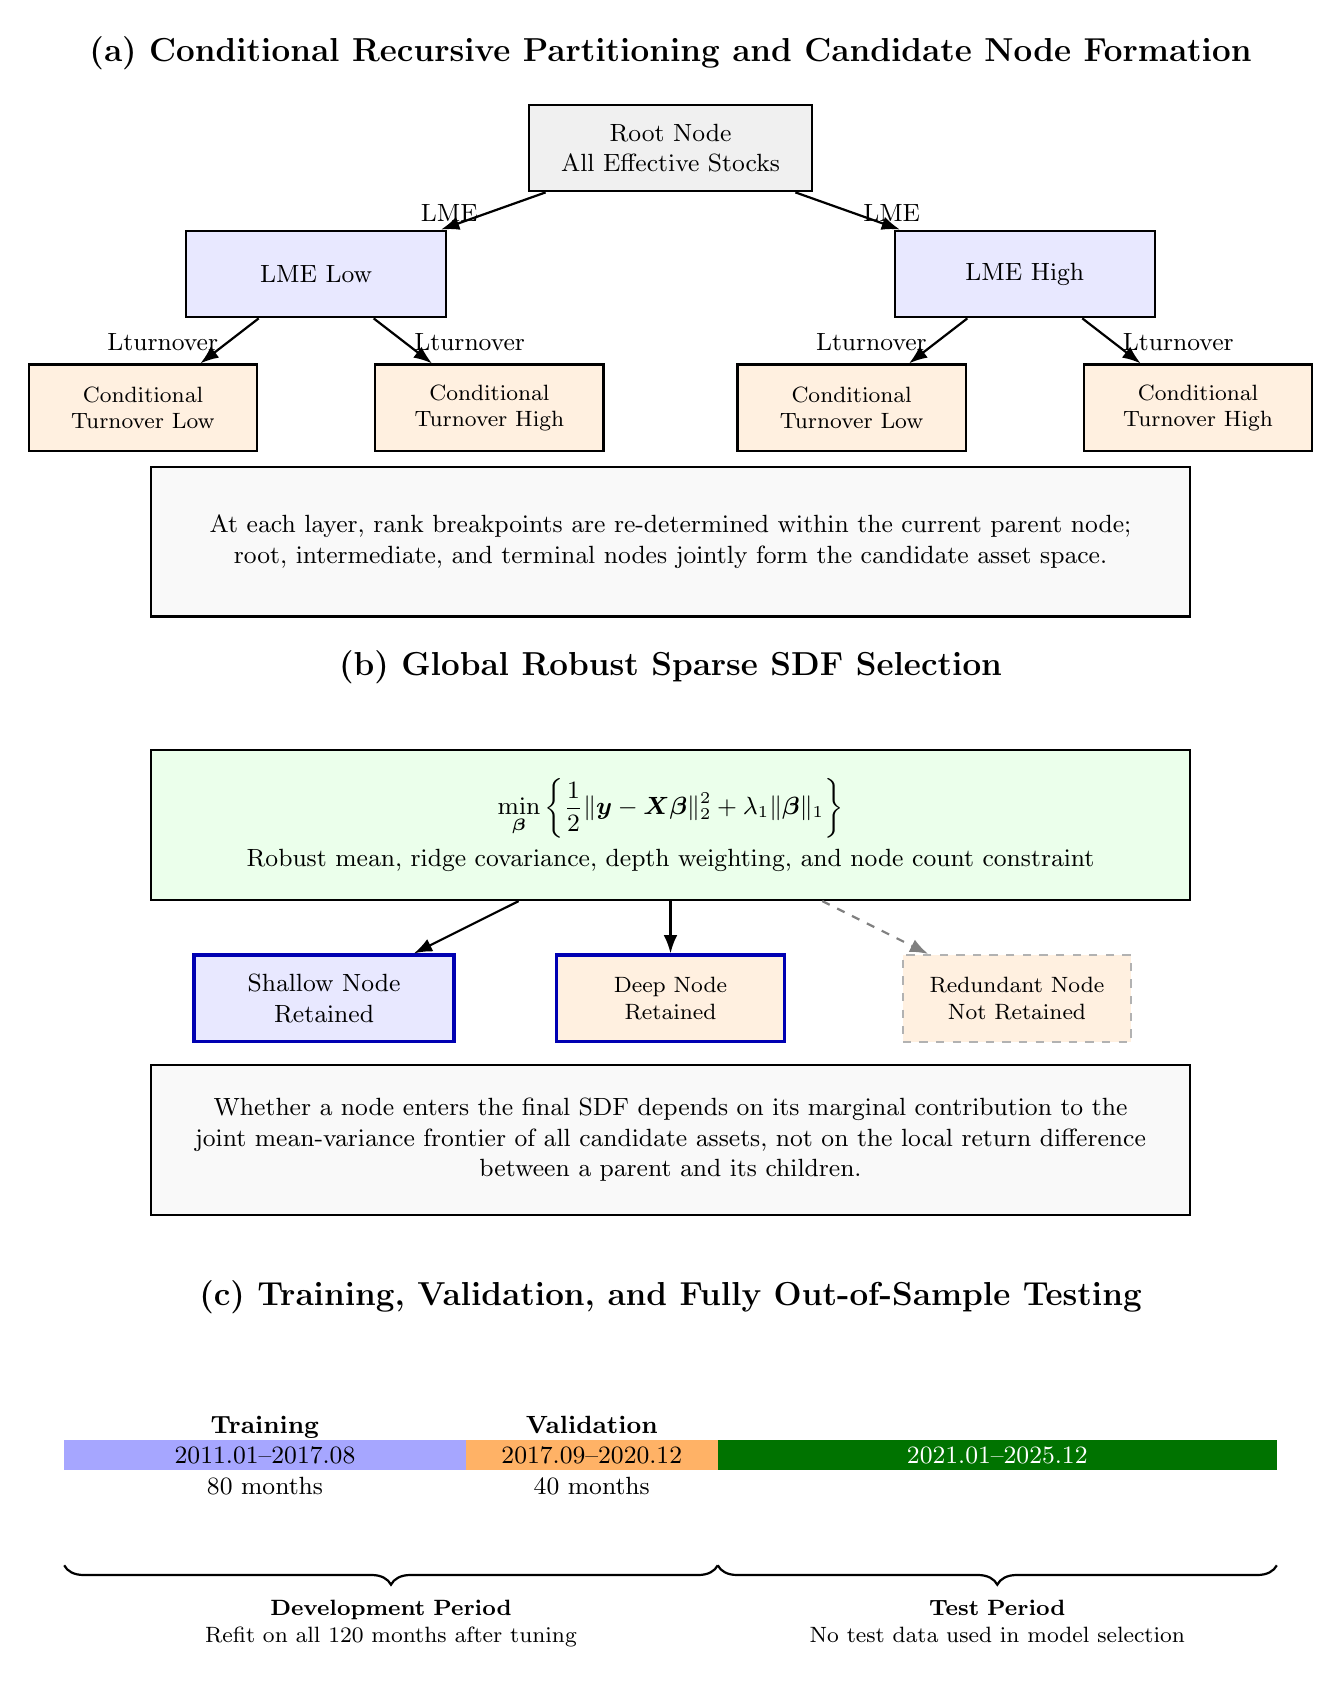
\begin{tikzpicture}[
    font=\small,
    >=Latex,
    root/.style={
      draw,
      fill=gray!12,
      minimum width=36mm,
      minimum height=11mm,
      align=center
    },
    parent/.style={
      draw,
      fill=blue!9,
      minimum width=33mm,
      minimum height=11mm,
      align=center
    },
    leaf/.style={
      draw,
      fill=orange!12,
      minimum width=29mm,
      minimum height=11mm,
      align=center,
      font=\footnotesize
    },
    box/.style={
      draw,
      minimum width=132mm,
      minimum height=19mm,
      align=center
    },
    every path/.style={line width=0.8pt}
  ]

  % ========== Panel (a) ==========
  \node[font=\bfseries\large] at (0,11.0)
    {(a) Conditional Recursive Partitioning and Candidate Node Formation};

  \node[root] (u) at (0,9.8)
    {Root Node\\All Effective Stocks};
  \node[parent] (l1) at (-4.5,8.2)
    {$\mathrm{LME}$ Low};
  \node[parent] (h1) at (4.5,8.2)
    {$\mathrm{LME}$ High};
  \node[leaf] (ll) at (-6.7,6.5)
  {Conditional\\Turnover Low};
  \node[leaf] (lh) at (-2.3,6.5)
    {Conditional\\Turnover High};
  \node[leaf] (hl) at (2.3,6.5)
    {Conditional\\Turnover Low};
  \node[leaf] (hh) at (6.7,6.5)
    {Conditional\\Turnover High};

  \draw[->] (u)--node[left,pos=.55]{$\mathrm{LME}$} (l1);
  \draw[->] (u)--node[right,pos=.55]{$\mathrm{LME}$} (h1);
  \draw[->] (l1)--node[left,pos=.52]{$\mathrm{Lturnover}$} (ll);
  \draw[->] (l1)--node[right,pos=.52]{$\mathrm{Lturnover}$} (lh);
  \draw[->] (h1)--node[left,pos=.52]{$\mathrm{Lturnover}$} (hl);
  \draw[->] (h1)--node[right,pos=.52]{$\mathrm{Lturnover}$} (hh);

  \node[box,fill=gray!5] at (0,4.8)
    {At each layer, rank breakpoints are re-determined within the current parent node;\\root, intermediate, and terminal nodes jointly form the candidate asset space.};

  % ========== Panel (b) ==========
  \node[font=\bfseries\large] at (0,3.2)
    {(b) Global Robust Sparse SDF Selection};

  \node[box,fill=green!8] (obj) at (0,1.2)
    {$\displaystyle
      \min_{\bm\beta}
      \left\{
        \frac{1}{2}\|\bm y-\bm X\bm\beta\|_2^2
        +\lambda_1\|\bm\beta\|_1
      \right\}$\\[1mm]
     Robust mean, ridge covariance, depth weighting, and node count constraint};

  \node[parent,draw=blue!70!black,line width=1.2pt]
    (keep1) at (-4.4,-1.0) {Shallow Node\\Retained};
  \node[leaf,draw=blue!70!black,line width=1.2pt]
    (keep2) at (0,-1.0) {Deep Node\\Retained};
  \node[leaf,draw=gray!60,dashed]
    (drop) at (4.4,-1.0) {Redundant Node\\Not Retained};

  \draw[->] (obj)--(keep1);
  \draw[->] (obj)--(keep2);
  \draw[->,dashed,gray] (obj)--(drop);

  \node[box,fill=gray!5] at (0,-2.8)
    {Whether a node enters the final SDF depends on its marginal contribution to the\\joint mean-variance frontier of all candidate assets, not on the local return difference\\between a parent and its children.};

  % ========== Panel (c) ==========
  \node[font=\bfseries\large] at (0,-4.8)
    {(c) Training, Validation, and Fully Out-of-Sample Testing};

  \coordinate (a) at (-7.7,-6.8);
  \coordinate (b) at (-2.6,-6.8);
  \coordinate (c) at (0.6,-6.8);
  \coordinate (d) at (7.7,-6.8);

  \draw[line width=11pt,blue!35] (a)--(b);
  \draw[line width=11pt,orange!60] (b)--(c);
  \draw[line width=11pt,green!45!black] (c)--(d);

  \node[align=center] at (-5.15,-6.8)
    {\textbf{Training}\\2011.01--2017.08\\80 months};
  \node[align=center] at (-1.0,-6.8)
    {\textbf{Validation}\\2017.09--2020.12\\40 months};
  \node[align=center,text=white] at (4.15,-6.8)
    {\textbf{Fully Out-of-Sample Test}\\2021.01--2025.12\\60 months};

  % Development-period annotation
  \draw[
    decorate,
    decoration={brace,amplitude=7pt,mirror}
  ]
    (a |- 0,-8.2) -- (c |- 0,-8.2)
    node[
      midway,
      below=9pt,
      align=center,
      font=\footnotesize,
      text width=62mm
    ]
    {\textbf{Development Period}\\
    Refit on all 120 months after tuning};

  % Fully out-of-sample annotation
  \draw[
    decorate,
    decoration={brace,amplitude=7pt,mirror}
  ]
    (c |- 0,-8.2) -- (d |- 0,-8.2)
    node[
      midway,
      below=9pt,
      align=center,
      font=\footnotesize,
      text width=54mm
    ]
    {\textbf{Test Period}\\
    No test data used in model selection};
  \end{tikzpicture}%
  }

  \caption{AP-Tree Conditional Splitting, Global Selection, and Sample Timeline}
  \label{fig:ap_tree_method}
  \begin{minipage}{0.94\textwidth}\footnotesize
  \textit{Note:}
  Panel (a) illustrates the first two splits using $\mathrm{LME}$ and $\mathrm{Lturnover}$.
  In practice, the candidate asset pool allows the three section characteristics to repeat over four layers, and retains parent and child nodes at different depths.
  Panel (b) shows that AP-Tree selects nodes jointly based on robust SDF spanning and sparsity in the full candidate asset space.
  Panel (c) displays the fixed time split; the test period is used only for fully out-of-sample evaluation.
  \end{minipage}
\end{figure}
\clearpage

\subsection{Factor Models and Asset Pricing Tests}
\label{subsec:factor_models_tests}

\subsubsection{Six Factor Models}

We select six benchmark factor models: CH3, CH4, FF5, FF6, Carhart4, and Q5. These models capture common variation in stock returns from dimensions such as market risk, size, value, profitability, investment, momentum, investor sentiment, and expected growth. For model \(m\in\mathcal M\), define the model set
\begin{equation}
  \mathcal M
  =
  \{\mathrm{CH3},\mathrm{CH4},\mathrm{FF5},
    \mathrm{FF6},\mathrm{Carhart4},\mathrm{Q5}\},
  \label{eq:factor_model_set}
\end{equation}
and let \(\bm f_t^{(m)}\in\mathbb R^{K_m}\) be the vector of factor returns in month \(t\) for model \(m\), with \(K_m\) factors.

CH3 is a three-factor model constructed for the Chinese stock market, including the market factor \(\mathrm{MKT}^{CH}\), the size factor \(\mathrm{SMB}^{CH}\), and the value factor \(\mathrm{VMG}^{CH}\). These measure the market excess return, the return difference between small and large stocks, and the difference between value and growth stocks based on earnings-to-price, respectively. The model accounts for shell-value contamination in the Chinese market \cite{ref17}:
\begin{equation}
  \bm f_t^{(\mathrm{CH3})}
  =
  \begin{pmatrix}
    \mathrm{MKT}_t^{CH}\\
    \mathrm{SMB}_t^{CH}\\
    \mathrm{VMG}_t^{CH}
  \end{pmatrix},
  \qquad K_{\mathrm{CH3}}=3.
  \label{eq:ch3}
\end{equation}

CH4 augments CH3 with a sentiment factor \(\mathrm{PMO}\), which measures the return difference between pessimistic and optimistic stocks, capturing pricing effects related to turnover, investor sentiment, and subsequent reversals in the Chinese market \cite{ref17}:
\begin{equation}
  \bm f_t^{(\mathrm{CH4})}
  =
  \begin{pmatrix}
    \mathrm{MKT}_t^{CH}\\
    \mathrm{SMB}_t^{CH}\\
    \mathrm{VMG}_t^{CH}\\
    \mathrm{PMO}_t
  \end{pmatrix},
  \qquad K_{\mathrm{CH4}}=4.
  \label{eq:ch4}
\end{equation}

FF5 includes the market factor \(\mathrm{MKT}^{FF}\), size factor \(\mathrm{SMB}^{FF}\), value factor \(\mathrm{HML}\), profitability factor \(\mathrm{RMW}\), and investment factor \(\mathrm{CMA}\). These capture market excess return, size, book-to-market, profitability, and investment styles \cite{ref10}:
\begin{equation}
  \bm f_t^{(\mathrm{FF5})}
  =
  \begin{pmatrix}
    \mathrm{MKT}_t^{FF}\\
    \mathrm{SMB}_t^{FF}\\
    \mathrm{HML}_t\\
    \mathrm{RMW}_t\\
    \mathrm{CMA}_t
  \end{pmatrix},
  \qquad K_{\mathrm{FF5}}=5.
  \label{eq:ff5}
\end{equation}
where \(\mathrm{HML}\) is high book-to-market minus low, \(\mathrm{RMW}\) is robust profitability minus weak, and \(\mathrm{CMA}\) is conservative investment minus aggressive.

FF6 augments FF5 with a momentum factor \(\mathrm{UMD}\), measuring the return difference between past winners and losers:
\begin{equation}
  \bm f_t^{(\mathrm{FF6})}
  =
  \begin{pmatrix}
    \mathrm{MKT}_t^{FF}\\
    \mathrm{SMB}_t^{FF}\\
    \mathrm{HML}_t\\
    \mathrm{RMW}_t\\
    \mathrm{CMA}_t\\
    \mathrm{UMD}_t
  \end{pmatrix},
  \qquad K_{\mathrm{FF6}}=6.
  \label{eq:ff6}
\end{equation}

Carhart4 includes the market factor \(\mathrm{MKT}^{FF}\), size factor \(\mathrm{SMB}^{FF}\), value factor \(\mathrm{HML}\), and momentum factor \(\mathrm{UMD}\) \cite{ref4}:
\begin{equation}
  \bm f_t^{(\mathrm{Carhart4})}
  =
  \begin{pmatrix}
    \mathrm{MKT}_t^{FF}\\
    \mathrm{SMB}_t^{FF}\\
    \mathrm{HML}_t\\
    \mathrm{UMD}_t
  \end{pmatrix},
  \qquad K_{\mathrm{Carhart4}}=4.
  \label{eq:carhart4}
\end{equation}

Q5 includes the market factor \(R_m-R_f\), size factor \(R_{\mathrm{ME}}\), investment factor \(R_{\mathrm{IA}}\), profitability factor \(R_{\mathrm{ROE}}\), and expected growth factor \(R_{\mathrm{EG}}\). These capture market excess return, the return difference between small and large stocks, low versus high investment firms, high versus low profitability firms, and high versus low expected growth firms \cite{ref23,ref24}:
\begin{equation}
  \bm f_t^{(\mathrm{Q5})}
  =
  \begin{pmatrix}
    R_{m,t}-R_{f,t}\\
    R_{\mathrm{ME},t}\\
    R_{\mathrm{IA},t}\\
    R_{\mathrm{ROE},t}\\
    R_{\mathrm{EG},t}
  \end{pmatrix},
  \qquad K_{\mathrm{Q5}}=5.
  \label{eq:q5}
\end{equation}
All factor returns are exogenous monthly benchmark series that do not participate in AP-Tree node generation, hyperparameter selection, or weight estimation; they are used only for asset pricing evaluation of the section SDFs and their selected nodes in the test period.

\subsubsection{Time-Series Regression of Section SDF}

For section \(s\in\mathcal S\) and factor model \(m\in\mathcal M\), estimate in the test period
\begin{equation}
  R_{s,t}^{\mathrm{SDF},e}
  =
  \alpha_s^{(m)}
  +\bm\beta_s^{(m)\top}\bm f_t^{(m)}
  +\varepsilon_{s,t}^{(m)},
  \qquad
  t\in\mathcal T_{\mathrm{test}},
  \label{eq:sdf_factor_regression}
\end{equation}
where \(\alpha_s^{(m)}\) is the monthly pricing intercept, \(\bm\beta_s^{(m)}\in\mathbb R^{K_m}\) is the factor loading vector, and \(\varepsilon_{s,t}^{(m)}\) is the regression residual. The annualized intercept is
\begin{equation}
  \widehat\alpha_{s,\mathrm{ann}}^{(m)}
  =
  12\widehat\alpha_s^{(m)}.
  \label{eq:annual_alpha}
\end{equation}
The time-series \(R^2\) measures the fraction of monthly variation in the section SDF explained by the benchmark factors. A high annualized \(\alpha\) indicates that the portfolio retains a high average return after controlling for benchmark factors; a low time-series \(R^2\) indicates that its return variation is harder to replicate by the benchmark model. Inference for intercepts uses Newey--West heteroskedasticity and autocorrelation robust standard errors.

\subsubsection{XS-\(R^2\) of Selected Nodes}

To avoid the final portfolio weights masking pricing errors of underlying test assets, we further estimate for each selected node \(j\in\widehat{\mathcal J}_s\) of section \(s\):
\begin{equation}
  R_{s,j,t}^{e}
  =
  \alpha_{s,j}^{(m)}
  +\bm\beta_{s,j}^{(m)\top}\bm f_t^{(m)}
  +\varepsilon_{s,j,t}^{(m)},
  \qquad
  t\in\mathcal T_{\mathrm{test}},
  \label{eq:node_factor_regression}
\end{equation}
where \(\alpha_{s,j}^{(m)}\) is the monthly pricing intercept of node \(j\), and \(\bm\beta_{s,j}^{(m)}\in\mathbb R^{K_m}\) is its factor loading vector. This test uses the node's own test-period raw excess returns, without depth transformation or multiplication by the final SDF weight.

Let \(N_s=|\widehat{\mathcal J}_s|\) be the number of selected nodes, and require \(N_s>K_m\). The test-period average excess return of node \(j\) is
\begin{equation}
  \overline R_{s,j}^{e}
  =
  \frac{1}{T_{\mathrm{test}}}
  \sum_{t\in\mathcal T_{\mathrm{test}}}
  R_{s,j,t}^{e}.
  \label{eq:node_mean_excess_return}
\end{equation}
The degrees-of-freedom adjusted cross-sectional explanatory power is
\begin{equation}
  \begin{aligned}
  \mathrm{XS}\text{-}R_{s,m}^{2}
  =1-
  \frac{N_s}{N_s-K_m}
  \frac{
    \displaystyle
    \sum_{j\in\widehat{\mathcal J}_s}
    \bigl(\widehat\alpha_{s,j}^{(m)}\bigr)^2
  }{
    \displaystyle
    \sum_{j\in\widehat{\mathcal J}_s}
    \bigl(\overline R_{s,j}^{e}\bigr)^2
  }.
  \end{aligned}
  \label{eq:xs_r2}
\end{equation}
A low XS-\(R^2\) indicates that the benchmark factors have difficulty explaining the cross-sectional average returns of the selected nodes. Because the measure includes degrees-of-freedom adjustment and uses the uncentered sum of squared average returns as denominator, it can be negative. A negative value means that the adjusted sum of squared pricing errors exceeds the sum of squared average excess returns.

\subsubsection{GRS Joint Test}

In addition to section-by-section regressions, we test whether the pricing intercepts of the 36 section SDFs under the same strategy are jointly zero. Let \(N=|\mathcal S|=36\), and write the test asset excess returns as
\begin{equation}
  \bm r_t^{S,e}
  =
  \bm\alpha^{(m)}
  +\bm B^{(m)}\bm f_t^{(m)}
  +\bm\varepsilon_t^{(m)},
  \qquad
  t\in\mathcal T_{\mathrm{test}},
  \label{eq:grs_system}
\end{equation}
where \(\bm r_t^{S,e}\in\mathbb R^N\) is the vector of 36 section SDF excess returns, \(\bm\alpha^{(m)}\in\mathbb R^N\) is the intercept vector, \(\bm B^{(m)}\in\mathbb R^{N\times K_m}\) is the factor loading matrix, and \(\bm\varepsilon_t^{(m)}\in\mathbb R^N\) is the residual vector.

Let \(T=T_{\mathrm{test}}\), and define the factor sample mean, factor sample covariance, and residual sample covariance as
\begin{align}
  \overline{\bm f}^{(m)}
  &=
  \frac{1}{T}
  \sum_{t\in\mathcal T_{\mathrm{test}}}
  \bm f_t^{(m)},
  \label{eq:factor_sample_mean}\\
  \widehat{\bm\Omega}_{f}^{(m)}
  &=
  \frac{1}{T}
  \sum_{t\in\mathcal T_{\mathrm{test}}}
  \bigl(
    \bm f_t^{(m)}-\overline{\bm f}^{(m)}
  \bigr)
  \bigl(
    \bm f_t^{(m)}-\overline{\bm f}^{(m)}
  \bigr)^{\top},
  \label{eq:factor_covariance}\\
  \widehat{\bm\Sigma}_{\varepsilon}^{(m)}
  &=
  \frac{1}{T}
  \sum_{t\in\mathcal T_{\mathrm{test}}}
  \widehat{\bm\varepsilon}_t^{(m)}
  \widehat{\bm\varepsilon}_t^{(m)\top}.
  \label{eq:residual_covariance}
\end{align}
When \(T>N+K_m\) and the relevant covariance matrices are invertible, the GRS statistic is
\begin{equation}
  \begin{aligned}
  \mathrm{GRS}^{(m)}
  ={}&
  \frac{T}{N}
  \frac{T-N-K_m}{T-K_m-1}\\
  &\times
  \frac{
    \widehat{\bm\alpha}^{(m)\top}
    \bigl(\widehat{\bm\Sigma}_{\varepsilon}^{(m)}\bigr)^{-1}
    \widehat{\bm\alpha}^{(m)}
  }{
    1+
    \overline{\bm f}^{(m)\top}
    \bigl(\widehat{\bm\Omega}_{f}^{(m)}\bigr)^{-1}
    \overline{\bm f}^{(m)}
  }.
  \end{aligned}
  \label{eq:grs_statistic}
\end{equation}
The null hypothesis is
\begin{equation}
  H_0:
  \bm\alpha^{(m)}=\bm 0_N.
  \label{eq:grs_null}
\end{equation}
Under the classical GRS assumptions of normality, homoskedasticity, and independence, under the null,
\begin{equation}
  \mathrm{GRS}^{(m)}
  \sim
  F_{N,\,T-N-K_m}.
  \label{eq:grs_distribution}
\end{equation}
A small \(p\)-value indicates that the benchmark factor model cannot simultaneously explain the average returns of the 36 section SDFs. The GRS test measures the joint significance of intercepts and does not directly evaluate the economic magnitude, Sharpe ratio, or drawdown of portfolio returns; it should therefore be interpreted together with out-of-sample performance metrics.

\subsection{Summary of Method Specifications}
\label{subsec:method_summary}

We compare TripleSort64 with four AP-Tree specifications. The AP-Tree specification set is
\begin{equation}
  \begin{aligned}
  \mathcal A
  =\{\,&(K_{\max}=20,\ \text{Deep Boost}),
         (K_{\max}=20,\ \text{Shallow Tilt}),\\
       &(K_{\max}=40,\ \text{Deep Boost}),
         (K_{\max}=40,\ \text{Shallow Tilt})\}.
  \end{aligned}
  \label{eq:ap_tree_strategy_set}
\end{equation}
All strategies are evaluated on the same 36 three-characteristic cross-sections and the same training–validation–testing chronology. AP-Tree is run with \(K_{\max}=20\) and \(K_{\max}=40\), comparing Deep Boost and Shallow Tilt. The comparison across methods reflects not only differences in candidate asset counts, but also differences in conditional recursive partitioning, overlapping parent–child node structure, and depth preference.

In summary, our methodology unifies three levels of questions within a single framework: the candidate-pool stage uses conditional recursive partitioning to approximate the mapping from firm characteristics to conditional SDF loadings; the sparse selection stage uses robust moments and generalized least-squares transformation to recover a sparse section SDF from all parent and child nodes; the testing stage uses fully out-of-sample Sharpe ratios, factor-adjusted \(\alpha\), time-series \(R^2\), node-level XS-\(R^2\), and the GRS joint test to evaluate the incremental pricing information contained in the candidate cross-sections. Deep Boost and Shallow Tilt are used to examine the trade-off between local interaction information and portfolio diversification.

\clearpage

\section{Empirical Results}
\label{sec:empirical_results}

This section first examines the fully out-of-sample performance of each specification in the raw sample, and uses this to identify potential contamination from micro-caps and shell value. We then re-evaluate each strategy after monthly exclusion of the lowest \(30\%\) of stocks by market capitalization, comparing the impact of sample cleaning on different portfolio construction methods. In the cleaned sample, we further compare Deep Boost and Shallow Tilt to examine how depth preference affects returns, risk, and asset pricing performance under different sparsity levels. Subsequently, we report factor model tests, GRS joint tests, node attribution of high-Sharpe SDFs, long-only results, and portfolio turnover.

\subsection{Depth Preference: Economic Trade-off and Testable Implications}
\label{subsec:depth_weight_hypothesis}

Node depth weighting reflects the fundamental trade-off between diversification and local information. Shallow nodes cover many stocks and thus are more likely to diversify firm-specific idiosyncratic noise; deep nodes have narrower coverage but can capture cross-sectional return differentials that emerge only after successive conditional splits. The original AP-Tree favors the former mechanism. If node \(i\) contains \(N_i\) stocks and idiosyncratic noise decays at rate \(1/N_i\), the standard error of node returns declines roughly as \(1/\sqrt{N_i}\), and the corresponding GLS intuition supports scaling nodes by \(\sqrt{N_i}\). For an approximately balanced binary tree, since \(N_i\propto 2^{-d_i}\), this specification is equivalent to scaling down deep nodes by \(2^{-d_i/2}\). We call this \emph{Shallow Tilt}.

Whether this diversification logic applies directly to the Chinese market is not obvious. Expanding node coverage can reduce firm-specific noise, but may not diversify common fluctuations from policy shocks, industry co-movements, and changing market states. Meanwhile, if pricing information mainly resides in local regions jointly determined by size, historical returns, and trading frictions, shallow portfolios may merge stocks with different economic meanings and attenuate the relevant cross-sectional return differentials. Thus, the noise reduction from broader coverage may come at the cost of losing local pricing information.

We use \emph{Deep Boost} to test the latter possibility. This transformation raises the relative scale of deep nodes when they enter the sparse selection path, making it easier for the model to retain narrower-coverage but information-richer portfolios. Consequently, Shallow Tilt and Deep Boost correspond to two competing hypotheses: the former assumes that diversification benefits dominate node selection, while the latter assumes that local conditional information is sufficient to compensate for the extra noise borne by smaller nodes. We do not presume either mechanism to be dominant, but leave their relative importance to be judged by out-of-sample evidence.

Our empirical analysis evaluates the above hypotheses from both return and pricing dimensions. The return dimension examines out-of-sample returns and maximum drawdown; the pricing dimension examines factor-adjusted \(\alpha\), time-series \(R^2\), XS-\(R^2\), and the GRS joint test. If Shallow Tilt performs better, the diversification advantage of broad-coverage nodes is the main source of SDF construction; if Deep Boost performs better, the conventional down-weighting of deep nodes may omit incremental pricing information contained therein. The two depth weightings and the rescaling to original scale were defined in Section~\ref{subsec:depth_weight}; here we only discuss their testable economic implications.

\subsection{Raw Sample: Limited Relative Advantage and Shell-Value Clues}
\label{subsec:full_sample}

Panel A of Figure~\ref{fig:full_sharpe} compares the out-of-sample monthly Sharpe ratios of TripleSort64 and the four AP-Tree specifications across the 36 characteristic cross-sections in the raw sample. Unlike the original U.S. evidence for AP-Tree, AP-Tree does not display an overwhelming advantage in the raw A-share sample. The five curves cross in many sections; TripleSort64 achieves comparable or even higher out-of-sample Sharpe ratios in several sections. Although conditional recursive partitioning alters the candidate asset space, it does not necessarily generate stable out-of-sample returns when characteristic signals are weak.

High-Sharpe strategies are concentrated in the characteristic dimension. The better-performing sections mostly include short-term reversal (ST\_Rev), turnover (Lturnover), or momentum (\(r12\_2\)); by contrast, sections composed of fundamental variables such as investment, profitability, accruals, and book-to-market are generally in the lower part of the distribution. Thus, AP-Tree's main role in the raw sample is to condition and localize existing trading signals, rather than replacing the economic information of characteristics with nonlinear structures.

\begin{figure}[htbp]
  \centering
  \includegraphics[width=0.98\textwidth]
  {output/figures/main/03_Full_Sharpe_By_Section.pdf}
  \caption{Out-of-Sample Monthly Sharpe Ratios in Raw and Cleaned Samples}
  \label{fig:full_sharpe}
  \begin{minipage}{0.96\textwidth}\footnotesize
  \textit{Note:} Panel A and Panel B report results for the raw sample and the cleaned sample after monthly exclusion of the lowest \(30\%\) of stocks by market capitalization, respectively. Within each panel, the 36 sections are ordered by the out-of-sample monthly Sharpe ratio of TripleSort64 from low to high. AP-Tree specifications are shown for \(K_{\max}=20\) and \(K_{\max}=40\) under Deep Boost and Shallow Tilt. The test period is January 2021–December 2025.
  \end{minipage}
\end{figure}

To examine whether the high Sharpe ratios in the raw sample depend on micro-caps, we further analyze the three SDFs with the highest out-of-sample monthly Sharpe ratios among all raw-sample strategies. Table~\ref{tab:top3_full} shows that the top-ranked is Sec09, the AP-Tree \(K_{\max}=20\) Deep Boost using LME, ST\_Rev, and \(r12\_2\); the second is Sec01, TripleSort64 using LME, Lturnover, and ST\_Rev; the third is Sec12, TripleSort64 using LME, ST\_Rev, and Fin\_Investment.

The three sections correspond to different economic mechanisms. Sec09 captures recursive interactions among relative size, last-month return, and medium-term momentum, testing whether short-term reversal depends on the stock's medium-term return state. Sec01 combines turnover and short-term reversal, capturing the joint state of trading activity and recent price changes. Sec12 combines short-term reversal with investment characteristics, examining whether the return implications of recent price changes differ across firms with different investment states. Despite different auxiliary characteristics, all three sections include LME and ST\_Rev, providing a common diagnostic dimension: whether the high Sharpe ratios mainly come from short-term reversal returns in the smallest stocks.

\begin{table}[htbp]
\centering
\caption{Top Three Raw-Sample SDFs by Out-of-Sample Monthly Sharpe Ratio}
\label{tab:top3_full}
\resizebox{\textwidth}{!}{%
\begin{tabular}{clllrrrrrr}
\hline
Rank & Section & Characteristic Set & Specification
& Monthly SR & Avg Monthly Excess Return & Max Drawdown
& Annual \(\alpha\) Range & TS-\(R^2\) Range & Selected Nodes \\
\hline
1 & Sec09
& LME, ST\_Rev, \(r12\_2\)
& AP-Tree \(K_{\max}=20\) Deep Boost
& 0.781 & 0.934\% & \(-0.93\%\)
& 8.54--10.94\% & 5.0--13.6\% & 20 \\

2 & Sec01
& LME, Lturnover, ST\_Rev
& TripleSort64
& 0.767 & 1.066\% & \(-3.92\%\)
& 9.74--12.90\% & 1.6--31.1\% & 16 \\

3 & Sec12
& LME, ST\_Rev, Fin\_Investment
& TripleSort64
& 0.757 & 0.923\% & \(-3.34\%\)
& 7.56--10.90\% & 3.5--32.2\% & 16 \\
\hline
\end{tabular}}
\begin{minipage}{0.96\textwidth}\footnotesize
\textit{Note:} Rankings are based on monthly Sharpe ratios in the test period across all raw-sample TripleSort64 and AP-Tree specifications. Annual \(\alpha\) and time-series \(R^2\) (TS-\(R^2\)) ranges are computed across the CH3, CH4, FF5, FF6, Carhart4, and Q5 benchmark models. AP-Tree Deep Boost corresponds to depth parameter \(p=0.5\).
\end{minipage}
\end{table}

Table~\ref{tab:top3_full} also shows that AP-Tree's relative advantage in the raw sample is limited. TripleSort64 occupies two of the top three positions, and Sec01 and Sec12 both achieve high average monthly excess returns. The top-ranked AP-Tree has a smaller maximum drawdown, but this does not imply that AP-Tree is universally superior across all 36 sections. More importantly, whether these three high-Sharpe combinations reflect generalizable characteristic interactions or mainly capture the special returns of the smallest A-share stocks remains to be determined.

Figure~\ref{fig:full_weight_cubes} maps the node weights of the three SDFs onto their respective three-dimensional characteristic spaces. The color at each position represents the sum of SDF weights across all selected nodes covering that position, rather than the weight of a single leaf node; positive and negative colors correspond to long and short sides of the final SDF. The gray plane marks the 30th percentile of full-market LME, below which lie the lowest \(30\%\) of stocks by market capitalization, i.e., the micro-cap region potentially affected by shell value.

\begin{figure}[htbp]
  \centering
  \includegraphics[width=0.99\textwidth]
  {output/figures/main/13_Full_TopSDF_WeightCubes_Combined.pdf}
  \caption{Weight Structure of Top Three Raw-Sample SDFs by Out-of-Sample Monthly Sharpe Ratio}
  \label{fig:full_weight_cubes}
  \begin{minipage}{0.96\textwidth}\footnotesize
  \textit{Note:} The three panels correspond to the top three SDFs in Table~\ref{tab:top3_full}. Colors represent the sum of SDF weights across all selected nodes covering the same characteristic position; positive and negative colors indicate cumulative net positive and negative weights, respectively. The gray plane marks the 30th percentile of full-market LME; below the plane is the potential shell-value contamination region. Weights from overlapping nodes at each position are aggregated and lightly smoothed. Let \(p_i=|w_i|/\sum_j|w_j|\) be the normalized absolute weight of selected node \(i\); effective node count is \(\mathrm{Eff.\ N}=1/\sum_i p_i^2\). Sparsity is defined as \(\mathrm{Eff.\ N}/N\), where \(N\) is the nominal selected node count. Lower sparsity indicates that SDF weights are concentrated in fewer effective nodes.
  \end{minipage}
\end{figure}

Figure~\ref{fig:full_weight_cubes} shows that the positive-weight regions of all three optimal SDFs are to varying degrees concentrated below the gray plane, i.e., their long sides overlap significantly with the lowest \(30\%\) of full-market stocks. Further verification using unsmoothed node weights and full recursive paths confirms the same conclusion and reveals the specific ways in which the three SDFs are exposed to the lowest-cap region.

Sec09's AP-Tree \(K_{\max}=20\) Deep Boost selects 20 nodes with an effective node count of 11.5. The two largest positive-weight nodes correspond to paths that repeatedly enter low-cap branches and a path that first splits by \(r12\_2\) and then repeatedly enters low-cap branches, with weights 0.0968 and 0.0946, respectively. Both nodes concentrate long positions in the extremely low region of full-market LME, rather than merely showing a general small-to-mid cap tilt.

Sec01's TripleSort64 consists of independent quartile intersections of LME, Lturnover, and ST\_Rev. Its largest positive-weight cell lies in the lowest market-cap quartile with weight 0.1592. Because TripleSort64 uses unconditional market-cap breakpoints, this cell directly covers most stocks below the gray plane. Thus, although Sec01 may also contain turnover and short-term reversal information, its strongest long exposure still overlaps with the micro-cap region.

Sec12's TripleSort64 similarly allocates its main positive weights to the lowest market-cap quartile. The two largest positive-weight cells have weights 0.1650 and 0.1307, both lying below or substantially covering the gray plane. Fin\_Investment changes the weight distribution within the lowest-cap group but does not eliminate the concentrated long exposure to micro-caps.

Although the three optimal SDFs come from different methods and include different auxiliary characteristics, their weight structures share a common feature: the main positive weights significantly enter the lowest \(30\%\) of full-market market-cap stocks. This does not constitute causal identification of a shell-value effect, because the lowest-cap region may also carry liquidity, trading restrictions, and other unobserved risks. However, it provides a clear sample diagnostic: the high Sharpe ratios in the raw sample cannot distinguish between generalizable nonlinear pricing structures and institutional returns specific to Chinese micro-caps or shell value.

Based on this diagnostic, our subsequent cleaned-sample tests are not an ex post deletion of part of the raw SDF returns. Rather, we monthly exclude the lowest \(30\%\) of LME stocks, and re-determine all sorting breakpoints, generate AP-Tree nodes and TripleSort64 cells, select hyperparameters, and estimate SDF weights. Only if the out-of-sample performance persists after excluding the potential shell-value region can AP-Tree's advantage be more credibly attributed to conditional characteristic interactions rather than unconditional micro-cap exposure.

\subsection{Cleaned Sample: Sharpe Changes after Removing Shell-Value Contamination}
\label{subsec:cleaned_sample}

\begin{figure}[htbp]
  \centering
  \includegraphics[width=0.99\textwidth]
  {output/figures/main/12_Full_Cleaned_Sharpe_Combined.pdf}
  \caption{Out-of-Sample Monthly Sharpe Ratios in Raw and Cleaned Samples}
  \label{fig:full_clean_sharpe}
  \begin{minipage}{0.96\textwidth}\footnotesize
  \textit{Note:} Panel A reports raw-sample results; Panel B reports cleaned-sample results after monthly exclusion of the lowest \(30\%\) of stocks by market capitalization and re-estimation. Within each panel, the 36 sections are ordered by the TripleSort64 out-of-sample monthly Sharpe ratio in that sample from low to high, so the horizontal positions are not directly comparable across panels. AP-Tree specifications are shown for \(K_{\max}=20\) and \(K_{\max}=40\) under Deep Boost and Shallow Tilt.
  \end{minipage}
\end{figure}

Figure~\ref{fig:full_clean_sharpe} provides the main sample diagnostic of this section. After excluding the lowest-cap stocks, TripleSort64's out-of-sample monthly Sharpe ratio declines most markedly. In the raw sample, TripleSort64 reaches or exceeds AP-Tree in several sections and is highly competitive in the high-Sharpe region; in the cleaned sample, its curve shifts downward overall and lies below the four AP-Tree specifications in most sections. In contrast, although AP-Tree's Sharpe ratios also decline, its cross-sectional ranking and high-Sharpe specifications are more stable.

This difference indicates that TripleSort64's raw-sample performance depends more heavily on the lowest-cap cells. Fixed cross-sorting concentrates micro-cap or shell-value returns in a few extreme portfolios; after excluding those stocks, the associated returns attenuate substantially. This does not mean that AP-Tree is unaffected by micro-caps, but rather that its decline is relatively smaller. By forming local assets through conditional recursive partitioning, AP-Tree's performance is not primarily driven by unconditional lowest-cap exposure. After excluding the potential shell-value region and re-estimating all models, some characteristic interactions still generate high out-of-sample risk-adjusted returns. Appendix Figure~\ref{fig:performance_boxplots} further reports the distribution of three performance metrics across all 36 sections. AP-Tree's relative performance is not driven solely by a single extreme section, but there remains notable cross-sectional heterogeneity across specifications.
\clearpage

\subsection{Deep Boost versus Shallow Tilt}
\label{subsec:depth_comparison}

Figure~\ref{fig:depth_comparison} compares Deep Boost and Shallow Tilt within the same characteristic section and the same \(K_{\max}\). All differences shown are Deep Boost minus Shallow Tilt: Panels A and D report differences in out-of-sample monthly Sharpe ratios, Panels B and E report differences in average monthly excess returns, and Panels C and F report differences in maximum drawdown. Since maximum drawdown is non-positive, a positive difference means Deep Boost has a shallower drawdown. Panels A–C correspond to \(K_{\max}=20\), Panels D–F to \(K_{\max}=40\).

\begin{figure}[htbp]
  \centering
  \includegraphics[width=0.98\textwidth]
  {output/figures/main/02_Depth_Weight_Performance_Differences.pdf}
  \caption{Out-of-Sample Performance Differences: Deep Boost minus Shallow Tilt}
  \label{fig:depth_comparison}
  \begin{minipage}{0.96\textwidth}\footnotesize
  \textit{Note:} All differences are Deep Boost minus Shallow Tilt. Panels A–C correspond to \(K_{\max}=20\); Panels D–F correspond to \(K_{\max}=40\). Maximum drawdown is non-positive, so a positive difference indicates a shallower drawdown for Deep Boost. Within each panel, sections are ordered by the corresponding difference from low to high; the horizontal order is not directly comparable across panels.
  \end{minipage}
\end{figure}

The main conclusion from Figure~\ref{fig:depth_comparison} is that the differences between the two depth weightings are most pronounced under tight sparsity constraints. When \(K_{\max}=20\), Deep Boost achieves a higher out-of-sample monthly Sharpe ratio in 23 of the 36 sections and a higher average monthly excess return in 26 sections. Its advantage comes mainly from the return side, rather than a general improvement in downside risk: Deep Boost has a shallower maximum drawdown in only 13 sections. This suggests that raising the scale of deep nodes does not uniformly reduce portfolio risk, but rather affects which return information is prioritized in the limited support set. Node depth weighting thus has an economic meaning beyond technical scaling: it changes the model's choice between shallow diversification and deep local signals.

Sec09 provides the clearest illustration. This section consists of LME, ST\_Rev, and \(r12\_2\). Under \(K_{\max}=20\), Deep Boost's out-of-sample monthly Sharpe ratio is 0.703, 0.090 higher than Shallow Tilt's 0.613. The node paths indicate that this difference does not arise from mechanically reweighting the same support set. Deep Boost selects 20 nodes, all at depth 4; in contrast, Shallow Tilt's support set includes broader nodes at depths 1, 2, and 3, replacing some terminal combinations with these wider nodes. Although both specifications have the same nominal node count of 20, Deep Boost's effective node count is 12.2, higher than Shallow Tilt's 10.4. Thus, raising the scale of deep nodes does not concentrate the SDF into fewer positions; instead, it allows the limited support set to cover more distinct local states. The difference between the two depth weightings thus goes beyond whether selected nodes are deep or shallow; it also reflects how limited model capacity is allocated between broad common components and local conditional information.

The specific paths of Sec09 reveal the economic content of these local states. Deep Boost assigns large positive weights to nodes that repeatedly enter low-LME branches, and to nodes that first split by \(r12\_2\) and then enter low-LME and ST\_Rev branches; negative weights appear in opposite regions defined by different medium-term momentum and recent return paths. Thus, Deep Boost preserves not an unconditional small-cap or reversal portfolio, but a short-term reversal within small-cap stocks that depends on medium-term price paths. When Shallow Tilt introduces broader intermediate nodes, it partially pools these local long-short differences, and the out-of-sample Sharpe ratio declines. Sec09 thus translates the average result in the figure into a clear mechanism: when short-term reversal holds only under specific size and momentum states, down-weighting deep nodes smooths the relevant conditional signals before they enter the limited support set. The economic role of node depth weighting is precisely to change the likelihood that these local signals are retained by the model.

This interpretation is also supported by cross-sectional pricing tests. Under \(K_{\max}=20\), Sec09's Deep Boost yields XS-\(R^2\) values of \(-0.159\), \(-0.017\), \(-0.678\), \(-0.798\), \(-0.767\), and \(-0.769\) under CH3, CH4, FF5, FF6, Carhart4, and Q5, respectively; all six estimates are negative. Shallow Tilt's corresponding range is \([-0.438,0.455]\). Negative adjusted XS-\(R^2\) indicates that the benchmark models fit the average returns of the selected nodes worse than a cross-sectional mean benchmark. Deep Boost thus simultaneously improves the out-of-sample Sharpe ratio of the final SDF and selects local assets that are difficult to span by any of the six mainstream factor models. This set of results is hard to reconcile with mere repackaging of existing factor exposures, and is more consistent with the hypothesis that deep nodes contain incremental cross-sectional pricing information.

When \(K_{\max}=40\), Deep Boost achieves a higher out-of-sample Sharpe ratio in only 14 sections, although it still dominates in average returns and maximum drawdown in 20 and 19 sections, respectively. Sec09 itself reflects this change: after expanding the support set from 20 to 40, the out-of-sample Sharpe ratios of Deep Boost and Shallow Tilt are 0.574 and 0.586, respectively, and the former 0.090 advantage disappears. A larger support set increases the coverage of the node space for both depth weightings, so the initial scale constraint on whether local states enter the SDF is relaxed; but additional nodes also raise estimation error and the risk of fitting in-sample noise and spurious covariances, so out-of-sample performance does not improve monotonically with capacity. Thus, expanding the support set can alleviate some node exclusion, but it does not eliminate the selection direction determined by depth weighting. The former mainly changes the trade-off between information coverage and estimation error; the latter mainly changes what type of information the model prioritizes. The two are related but non-substitutable.

Sec11 further illustrates that these two choices must match the information structure of the characteristic section. This section consists of LME, ST\_Rev, and IdioVol. Under \(K_{\max}=20\), Deep Boost's out-of-sample Sharpe ratio is 0.607, lower than Shallow Tilt's 0.646; when \(K_{\max}=40\), the figures are 0.721 and 0.704, respectively, and Deep Boost becomes the best-performing SDF in the cleaned sample. In the latter specification, Deep Boost's 40 nodes are all at depth 4, with an effective node count of 25.4; Shallow Tilt retains some root and intermediate nodes, with an effective node count of 21.1. The conditional role of idiosyncratic volatility on short-term reversal requires a sufficiently rich set of local states to recover: 20 nodes are insufficient to stably cover this structure, whereas 40 deep nodes can simultaneously accommodate more states of size, recent returns, and arbitrage risk. This does not imply that expanding the support set substitutes for Deep Boost; only when both are combined does the model have both the tendency to select local information and the capacity to accommodate it.

However, Sec11's increment is not accompanied by noticeably lower factor explanatory power. Under \(K_{\max}=40\), Deep Boost's SDF \(R^2\) range across the six models is 5.3\%--25.7\%, and its XS-\(R^2\) range is \([0.263,0.534]\); Shallow Tilt's corresponding ranges are 6.0\%--24.0\% and \([0.280,0.537]\). The factor fit of the two specifications is nearly identical. Thus, the 0.017 Sharpe difference in Sec11 is more likely due to a more effective combination of economically similar signals, rather than the discovery of a set of assets that are significantly harder to explain by existing models. This provides a discriminating contrast with Sec09: Sec09 shows that under strong sparsity constraints, depth weighting can determine whether new local pricing errors enter the support set; Sec11 shows that when the local structure itself requires larger capacity, the support-set size determines whether the model can fully cover those states.

In summary, the empirical advantage of Deep Boost has clear boundaries. When the support set is small, the relative scale of nodes directly affects which return signals enter the final SDF, so depth weighting effectively changes the model's trade-off between shallow diversification and deep local information; as \(K_{\max}\) increases, the model can cover more states but also faces higher estimation error. Sec09 shows that when capacity is limited, Deep Boost can preserve conditional short-term reversal that the shallow preference would smooth away; Sec11 shows that some local structures modulated by arbitrage risk require a larger support set to be fully recovered. Thus, deep nodes are not unconditionally superior to shallow ones, and expanding the support set cannot substitute for depth weighting. Out-of-sample performance ultimately depends on the match among node-selection direction, support-set capacity, and the economic structure of the section.

\subsection{Factor Model Explanatory Power}
\label{subsec:factor_evidence}
This section examines the explanatory power of CH4, FF5, and Q5 for the Section-SDFs. Figure~\ref{fig:factor_evidence} presents the results in a compact layout: the first, second, and third rows correspond to CH4, FF5, and Q5, respectively; the first, second, and third columns report the annualized \(\alpha\), time-series \(R^2\), and node-level XS-\(R^2\) of the Section-SDF.
\begin{figure}[p]
  \centering
  \includegraphics[
    width=0.94\textwidth,
    height=0.79\textheight,
    keepaspectratio
  ]{output/figures/main/11_Main_Factor_Evidence_Combined.pdf}
  \caption{Explanatory Power of Major Factor Models for Section-SDFs in Cleaned Sample}
  \label{fig:factor_evidence}
  \vspace{0.4em}

  \begin{minipage}{0.98\textwidth}
    \footnotesize
    \textit{Note:} Rows correspond to the Chinese four-factor model (CH4), Fama--French five-factor model (FF5), and the \(q\)-factor model (Q5); columns report annualized \(\alpha\), time-series \(R^2\), and node-level XS-\(R^2\) of the Section-SDF. Within each panel, sections are ordered separately by the corresponding metric of TripleSort64 from low to high, so the horizontal positions are not directly comparable across panels. Within each section, the five specifications are displayed in the same order; the horizontal ordering is determined only by TripleSort64 and does not indicate relative ordering of other specifications within the same section. Full results for CH3, FF6, and Carhart4 are provided in Appendix Figures~\ref{fig:appendix_factor_ch3}, \ref{fig:appendix_factor_ff6}, and \ref{fig:appendix_factor_carhart4}.
  \end{minipage}
\end{figure}
\clearpage

The first row of Figure~\ref{fig:factor_evidence} shows that CH4, which includes a sentiment factor, can explain a substantial portion of common variation in Section-SDFs, but does not universally eliminate abnormal returns. For example, Sec11 (LME, ST\_Rev, IdioVol) TripleSort64 has an annualized \(\alpha\) of \(5.18\%\) with a Newey–West \(t\)-statistic of 3.36, and a time-series \(R^2\) of \(40.87\%\). This indicates that while CH4 absorbs a large fraction of monthly volatility, the portfolio still retains a significant positive factor-adjusted return. At the same time, its node-level XS-\(R^2\) is \(56.06\%\), showing that ``the final portfolio has significant \(\alpha\)'' and ``the model can explain part of the cross-sectional average returns of nodes'' can hold simultaneously. More broadly, sections containing turnover or short-term reversal characteristics, such as Sec01, Sec02, Sec08–Sec12, and Sec23, tend to have higher TripleSort64 annualized \(\alpha\), while several sections composed of investment, profitability, and book-to-market lie in the lower region. CH4's time-series \(R^2\) peaks around \(65\%\), and node XS-\(R^2\) is mostly positive, with some AP-Tree specifications exceeding \(80\%\). Thus, CH4 has substantial explanatory power for many SDFs and node assets, but its coverage of trading-characteristic sections remains incomplete. Full regression results for the five sections with the highest CH4 time-series fit are reported in Appendix Table~\ref{tab:appendix_ch4_top5_r2}.

The second row of Figure~\ref{fig:factor_evidence} shows that FF5 has strong time-series coverage for several fundamental sections, but weaker explanatory power for high-return SDFs that contain turnover or short-term reversal characteristics. Sections Sec16, Sec17, Sec20, Sec21, and Sec34–Sec36 have relatively high time-series \(R^2\), peaking around \(76\%\); Sec10, Sec14, and others have noticeably lower fit. The stratification of annualized \(\alpha\) is also clear: TripleSort64 \(\alpha\) for fundamental sections like Sec24, Sec30, and Sec31 is close to zero, while Sec01, Sec02, Sec08, Sec11, and Sec12 lie in the higher region. Sec11's TripleSort64 annualized \(\alpha\) is \(7.75\%\) with a \(t\)-statistic of 4.69, time-series \(R^2\) of \(30.28\%\), and node XS-\(R^2\) of only \(1.84\%\). Thus, for this particular benchmark portfolio, FF5 not only fails to eliminate abnormal returns, but also barely explains the cross-sectional differences in average returns of its nodes. Appendix Table~\ref{tab:appendix_ff5_top5_r2} reports the annualized \(\alpha\), Newey–West \(t\)-statistics, and node-level XS-\(R^2\) for the five sections with the highest FF5 fit.

However, Sec11's low XS-\(R^2\) cannot be unconditionally generalized to all AP-Tree specifications of that section: its four AP-Tree specifications have FF5 XS-\(R^2\) around \(45.1\%\)–\(51.3\%\). This difference shows that cross-sectional explanatory power depends not only on the characteristic set but also on which nodes are ultimately selected by the construction method. Similarly, several trading-characteristic sections show negative XS-\(R^2\) for AP-Tree specifications, while many fundamental sections approach or exceed \(80\%\). FF5 thus more easily spans assets formed by traditional investment and profitability sorts, but lacks stable explanatory power for some local pricing directions identified by conditional recursive partitioning.

The third row of Figure~\ref{fig:factor_evidence} shows that Q5 has relatively high time-series explanatory power for sections related to medium-term returns, investment, and profitability, but this advantage does not stably translate into cross-sectional pricing ability. Sections Sec16–Sec21 and several fundamental sections have time-series \(R^2\) in the higher region, peaking near \(80\%\); sections containing turnover or short-term reversal are more often at the low end. Sec11's TripleSort64 again provides a direct example: its Q5 annualized \(\alpha\) is \(7.16\%\) with a \(t\)-statistic of 3.46, time-series \(R^2\) of only \(11.24\%\), and node XS-\(R^2\) of \(-23.13\%\). A negative XS-\(R^2\) means that Q5's prediction errors for these node average returns are worse than a cross-sectional mean benchmark. Sec11's four AP-Tree specifications all have positive Q5 XS-\(R^2\), around \(26.3\%\)–\(39.2\%\). The five sections with the highest Q5 time-series fit and their cross-sectional pricing results are reported in Appendix Table~\ref{tab:appendix_q5_top5_r2}.

Sec17 further shows that time-series fit and cross-sectional pricing are not equivalent. Its TripleSort64 has a Q5 annualized \(\alpha\) of \(-0.23\%\), time-series \(R^2\) of \(68.23\%\), but XS-\(R^2\) of \(-4.39\%\). Thus, even if Q5 nearly eliminates the abnormal return of the final SDF and explains a large fraction of monthly volatility, one cannot conclude that it spans the node assets that generate the SDF. Conversely, Sec09 shows that cross-sectional explanatory power also changes markedly with node selection: Q5's XS-\(R^2\) for TripleSort64 is \(29.27\%\), while for \(K_{\max}=20\) Deep Boost and Shallow Tilt it is \(-76.91\%\) and \(-43.83\%\), respectively. Therefore, the \(-0.769\) for Sec09 should be attributed specifically to the \(K_{\max}=20\) Deep Boost, not to TripleSort64.

Overall, the explanatory power of all three models exhibits significant cross-sectional heterogeneity. Sections composed of fundamental variables such as investment, profitability, and book-to-market generally have low annualized \(\alpha\) and high factor fit; sections containing ST\_Rev, Lturnover, or IdioVol are more likely to retain significant factor-adjusted returns and, in some AP-Tree specifications, produce low or even negative XS-\(R^2\). But this difference is neither a mechanical rule across all sections nor separable from the portfolio construction specification. Sec11 shows that a high-return SDF can retain significant \(\alpha\) under all three factor models, while node XS-\(R^2\) for the same section varies widely with the factor model and node selection; Sec17 shows that a high time-series \(R^2\) does not guarantee good cross-sectional pricing. Thus, our core evidence is not that any benchmark model is uniformly rejected along all dimensions, but rather that the explanatory power of existing models for local assets depends simultaneously on the characteristic section, the SDF construction method, and the spanning dimension examined. Full results for CH3, FF6, and Carhart4 are provided in Appendix Figures~\ref{fig:appendix_factor_ch3}, \ref{fig:appendix_factor_ff6}, and \ref{fig:appendix_factor_carhart4}.

\subsection{Global Best SDFs in Cleaned Sample and Sources of Mispricing}
\label{subsec:cleaned_best_sdf}

To identify the sources of return that persist after removing potential shell-value contamination, we perform a layered attribution of the high-performing AP-Tree SDFs in the cleaned sample. The first step selects the six SDFs with the highest out-of-sample monthly Sharpe ratios and comprehensively examines their returns, factor-adjusted performance, and cumulative weight structures of selected nodes in three-dimensional characteristic space. The second step expands the analysis to all AP-Tree specifications with out-of-sample monthly Sharpe ratios exceeding 0.55, comparing their major positive- and negative-weight nodes and recursive paths. The former characterizes the largest-magnitude local pricing structures, while the latter assesses whether these structures recur across node caps and depth weightings, avoiding economic interpretation that hinges on a single extreme specification.

To keep the main text from being crowded with node names and recursive paths, we only discuss nodes with relatively large weights and representative paths in the text. The complete list of selected nodes, depths, recursive paths, and final portfolio weights for the six highest-Sharpe SDFs is provided in Appendix Section~\ref{app:top6_node_weights}.

The threshold of out-of-sample monthly Sharpe ratio exceeding 0.55 yields 18 AP-Tree specifications. Under \(K_{\max}=20\), Deep Boost includes Sec09–Sec14; Shallow Tilt includes Sec09, Sec11, Sec12, and Sec13. Under \(K_{\max}=40\), both depth weightings include Sec09, Sec11, Sec12, and Sec13. All selected sections jointly contain LME and ST\_Rev, with the third characteristic being \(r12\_2\), LT\_Rev, IdioVol, Fin\_Investment, Fin\_OP, or Fin\_AC. The high-performing SDFs are thus not uniformly distributed across the 36 candidate sections, but concentrate in six sections centered on short-term price states, further conditioned by relative size and another state variable.

Among them, Sec09, Sec11, Sec12, and Sec13 exceed 0.55 under both \(K_{\max}\) and both depth weightings, constituting the most stable cross-specification evidence. Sec10 and Sec14 exceed the threshold only under \(K_{\max}=20\) Deep Boost, indicating that the incremental information from long-term return paths and accrual quality is more concentrated in a few deep conditional regions. Overall, the 18 high-Sharpe specifications first reveal a clear common fact: after excluding the lowest \(30\%\) of full-market stocks, the strongest unexplained returns still revolve around ST\_Rev, but the role of ST\_Rev is highly dependent on relative size and the state of historical returns, idiosyncratic risk, or firm fundamentals.

Table~\ref{tab:top6_cleaned} reports the six globally top-ranked SDFs. All six come from AP-Tree and retain significant positive \(\alpha\) under CH3, CH4, FF5, FF6, Carhart4, and Q5. The top three have out-of-sample monthly Sharpe ratios above 0.70; the top-ranked has a monthly Sharpe of 0.721, corresponding to an annualized Sharpe of about \(0.721\sqrt{12}=2.50\). All top six include ST\_Rev: three come from Sec11 (LME–ST\_Rev–IdioVol), two from Sec09 (LME–ST\_Rev–\(r12\_2\)), and one from Sec13 (LME–ST\_Rev–Fin\_OP). This concentration further narrows the subsequent mechanistic explanation to three dimensions: whether recent price pressure reverses, in which relative-size stocks this reversal is stronger, and how the third state variable distinguishes corrigible price pressure from economically justified price changes.

\begin{table}[htbp]
\centering
\caption{Top Six Cleaned-Sample SDFs by Out-of-Sample Monthly Sharpe Ratio}
\label{tab:top6_cleaned}
\resizebox{\textwidth}{!}{%
\begin{tabular}{cllrrrrrr}
\hline
Rank & Section & Specification & Monthly SR & Avg Monthly Excess Return & Max Drawdown
& Annual \(\alpha\) Range & TS-\(R^2\) Range & XS-\(R^2\) Range \\
\hline
1 & ST\_Rev--IdioVol & \(K_{\max}=40\) Deep Boost
 & 0.721 & 0.306\% & \(-1.14\%\)
 & 3.35--3.82\% & 5.3--25.7\% & 0.263--0.534 \\
2 & ST\_Rev--IdioVol & \(K_{\max}=40\) Shallow Tilt
 & 0.704 & 0.348\% & \(-1.21\%\)
 & 3.81--4.49\% & 6.0--24.0\% & 0.280--0.537 \\
3 & ST\_Rev--\(r12\_2\) & \(K_{\max}=20\) Deep Boost
 & 0.703 & 0.636\% & \(-2.74\%\)
 & 5.15--7.89\% & 3.0--29.1\% & \(-0.798\)--\(-0.017\) \\
4 & ST\_Rev--IdioVol & \(K_{\max}=20\) Shallow Tilt
 & 0.646 & 0.512\% & \(-1.76\%\)
 & 4.61--6.42\% & 4.0--30.1\% & 0.367--0.522 \\
5 & ST\_Rev--Fin\_OP & \(K_{\max}=40\) Shallow Tilt
 & 0.618 & 0.286\% & \(-0.84\%\)
 & 3.19--3.79\% & 6.2--14.3\% & 0.164--0.411 \\
6 & ST\_Rev--\(r12\_2\) & \(K_{\max}=20\) Shallow Tilt
 & 0.613 & 0.424\% & \(-2.31\%\)
 & 3.01--5.00\% & 3.5--27.7\% & \(-0.438\)--0.455 \\
\hline
\end{tabular}}
\begin{minipage}{0.96\textwidth}\footnotesize
\textit{Note:} Annual \(\alpha\), time-series \(R^2\) (TS-\(R^2\)), and XS-\(R^2\) ranges are computed across the CH3, CH4, FF5, FF6, Carhart4, and Q5 models. All six SDFs have significant \(\alpha\) at the \(5\%\) level across all six models. Monthly SR is the out-of-sample monthly Sharpe ratio in the test period.
\end{minipage}
\end{table}

The three types of metrics in the table identify different layers of model failure. First, all six SDFs retain significant positive \(\alpha\) under all six factor models, indicating that their high returns are not dependent on factor omissions of a single benchmark model. Second, the upper bound of time-series \(R^2\) is only \(30.1\%\), suggesting that existing factors can at best replicate part of the monthly variation of these SDFs. Third, the two \(K_{\max}=20\) specifications of Sec09 have notably low XS-\(R^2\); in particular, Deep Boost's XS-\(R^2\) is negative across all six models, ranging from \(-0.798\) to \(-0.017\). Thus, Sec09's evidence comes not only from the significant \(\alpha\) of the final SDF, but also from the inability of benchmark models to explain the average return differences among its selected nodes.

In contrast, Sec11 and Sec13 have mainly positive XS-\(R^2\). This means that benchmark factors can explain part of the cross-section of their underlying nodes, but still cannot replicate the dynamic long-short combination of the final SDF. The two cases correspond to different economic situations: Sec09 is closer to the discovery of local test assets that existing models cannot span; Sec11 and Sec13 are closer to extracting portfolio returns from partially spanable local assets that benchmark factors cannot replicate.

\begin{figure}[htbp]
  \centering
  \includegraphics[width=0.99\textwidth]
  {output/figures/main/14_Cleaned_TopSDF_WeightCubes_Combined.pdf}
  \caption{Cumulative Node Weight Structure of Top Six Cleaned-Sample SDFs}
  \label{fig:cleaned_weight_cubes}
  \begin{minipage}{0.96\textwidth}\footnotesize
  \textit{Note:} Green and red represent cumulative net positive and net negative weights, respectively. For each characteristic position, coefficients of all selected nodes covering that position are aggregated and lightly smoothed; thus the figure shows the cumulative node-weight field in characteristic space, not direct stock holdings. The LME axis in the cleaned sample corresponds to the 30th–100th percentiles of the original cross-sectional market-cap distribution, rescaled to full height. Eff.\ N is the effective node count based on standardized absolute node weights; Sparsity is Eff.\ N divided by nominal node count.
  \end{minipage}
\end{figure}

\subsubsection{Common Structure: Short-Term Reversal Conditional on Relative Size}

Figure~\ref{fig:cleaned_weight_cubes} reveals a recurring empirical structure across the top-ranked SDFs: ST\_Rev and LME jointly define the main positive and negative weight regions, while IdioVol, \(r12\_2\), and Fin\_OP further subdivide these regions. Several top SDFs allocate substantial cumulative positive weights to local regions with relatively low LME and low ST\_Rev within the cleaned sample, while several nodes defined by consecutive high-ST\_Rev branches receive large negative weights. This pattern is consistent with the predictive relation of short-term reversal, but is not equivalent to a simple two-dimensional sort. The figure also shows regions with opposite signs, and detailed node paths indicate that some larger weights appear only after the third variable intervenes or after further conditional splits by LME and ST\_Rev. Therefore, AP-Tree identifies not a uniform market-wide ``buy recent losers, sell recent winners'' but a nonlinear relation between ST\_Rev and subsequent returns that varies with relative size and other state variables.

Size here mainly acts as a conditioning variable, not an independent unconditional return source. The cleaning process already excludes the lowest \(30\%\) of full-market stocks each month, so low LME in node paths only indicates relatively low market cap within the remaining universe, no longer directly corresponding to extreme micro-caps or potential shell companies in the raw sample. After this screen, AP-Tree can still identify recurring conditional long-short structures within the remaining size distribution. This indicates that the high returns in the cleaned sample cannot be fully attributed to the direct contribution of excluded extreme micro-caps to portfolio returns.

However, the exclusion of micro-caps does not imply that all size-related economic channels have disappeared. LME still systematically participates in the recursive splitting of major nodes, indicating that the same ST\_Rev state has different subsequent return implications across different relative-size stocks. This size conditioning effect may be related to information environments, investor structure, liquidity, or arbitrage costs, but the current node results cannot distinguish among these channels. The directly supportable conclusion is that LME changes the conditional return relation of ST\_Rev, rather than independently generating a uniform small-cap premium across all stocks.

This structure is consistent with, but does not directly test, an interpretation based on limited arbitrage or non-fundamental trading demand causing temporary price deviations. Recent price changes may reflect adjustment to new information, but may also contain transitory trading demand; the further splits by IdioVol, \(r12\_2\), and Fin\_OP suggest that the subsequent performance of these recent-return states also depends on firm-specific volatility, historical return paths, and operating conditions. Since we do not directly observe order imbalance, investor attention, retail trading, short-sale constraints, or arbitrage capital, the node results themselves cannot determine the specific source of recent price changes, nor can they fully rule out state-dependent risk compensation. A more cautious empirical conclusion is that the strongest unexplained returns in the cleaned sample come from state-dependent short-term reversal, rather than from unconditional size effects or market-wide uniform short-term reversal.

\subsubsection{Sec11: Conditional Role of Idiosyncratic Volatility on Short-Term Reversal}

Sec11 is the strongest and most cross-specification stable section in the cleaned sample. Its \(K_{\max}=40\) Deep Boost and Shallow Tilt rank first and second globally, with out-of-sample monthly Sharpe ratios of 0.721 and 0.704; the \(K_{\max}=20\) Shallow Tilt ranks fourth with 0.646, and the \(K_{\max}=20\) Deep Boost also achieves 0.607. Thus, the high performance of the LME–ST\_Rev–IdioVol section does not depend on a single node cap or depth weighting.

Taking the top-ranked \(K_{\max}=40\) Deep Boost as an example, the largest positive-weight node corresponds to
\[
\text{Low LME}\rightarrow\text{High IdioVol}\rightarrow
\text{Low LME}\rightarrow\text{Low ST\_Rev},
\]
with node coefficient 0.0588. Another large positive-weight node is formed by sequential splits by ST\_Rev, LME, IdioVol, and ST\_Rev, with coefficient 0.0568. The largest negative-weight nodes include one formed by consecutive splits by ST\_Rev and LME, coefficient \(-0.0804\), and one formed by three consecutive high-ST\_Rev splits followed by a final LME split, coefficient \(-0.0786\). The second-ranked Shallow Tilt assigns different relative scales to nodes of different depths, but its main cumulative positive and negative weight regions are broadly similar to Deep Boost. This cross-depth similarity indicates that Sec11's high performance is not mechanically generated by a particular node-scaling rule.

These nodes also show that IdioVol does not have a stable unconditional weight direction. High IdioVol does not automatically correspond to positive node coefficients, nor automatically to negative ones; its sign depends on the preceding and subsequent LME and ST\_Rev splits. One large positive-weight node does appear in the conditional region of relatively low LME, high IdioVol, and low ST\_Rev, but other nodes containing high IdioVol states do not necessarily receive positive weights. Therefore, Sec11 cannot be interpreted as a simple reincarnation of the traditional high-idiosyncratic-volatility anomaly. More precisely, IdioVol changes the conditional relation between ST\_Rev and subsequent returns.

IdioVol may reflect firm-specific information uncertainty, investor disagreement, or arbitrage risk, so its interaction with ST\_Rev is compatible with a limited-arbitrage interpretation. For example, among stocks with high firm-specific uncertainty, the same recent return state may be more difficult for market participants to evaluate or trade in a timely manner. However, IdioVol itself may also contain fundamental risk and valuation uncertainty; we do not directly observe disagreement, short-sale constraints, or arbitrageur positions. Therefore, the existing results cannot determine whether the short-term reversal under high IdioVol comes from mispricing correction or state-dependent risk compensation. The direct conclusion supported by Sec11 is that idiosyncratic volatility has a significant conditional effect on short-term reversal, rather than that idiosyncratic volatility itself has a fixed expected return direction.

Sec11's factor tests further show that the abnormal return of the final SDF and the cross-sectional explainability of node assets are two distinct dimensions. Its best specification retains significant positive \(\alpha\) under all six factor models, while node XS-\(R^2\) remains positive. This means that benchmark factors can explain part of the average return differences among selected nodes, but cannot replicate AP-Tree's conditional selection and nonlinear combination of these nodes. Sec11's incremental information thus mainly lies in the conditional selection and nonlinear weighting of local assets, rather than requiring every underlying node to be a new anomaly unexplained by existing models.

\subsubsection{Sec09: Nonlinear Interaction between Short-Term and Medium-Term Return Paths}

Sec09 is another section that exceeds 0.55 under all four AP-Tree specifications. The \(K_{\max}=20\) Deep Boost and Shallow Tilt rank third and sixth globally, with out-of-sample monthly Sharpe ratios of 0.703 and 0.613; the two \(K_{\max}=40\) specifications have monthly Sharps of 0.574 and 0.586. Compared with Sec11, Sec09's evidence comes not only from higher final portfolio returns, but also from lower node-level cross-sectional explanatory power. In particular, the \(K_{\max}=20\) Deep Boost has negative XS-\(R^2\) under all six benchmark models, indicating that these models fit the average returns of the selected nodes worse than a cross-sectional mean benchmark.

In Sec09's \(K_{\max}=20\) Deep Boost, the largest positive-weight node enters low-LME branches three times and finally enters low-ST\_Rev, with coefficient 0.1209. Two other large positive-weight nodes have coefficients 0.1067 and 0.1037, similarly formed by repeated conditional splits of LME and ST\_Rev. The largest negative-weight node enters high-ST\_Rev three times and is finally split by LME, coefficient \(-0.1356\). These nodes together distribute cumulative positive weights more in the relatively low-LME, low-ST\_Rev region, and form stronger negative weights in some consecutive high-ST\_Rev regions.

However, the role of \(r12\_2\) cannot be reduced to a traditional medium-term momentum position. The selected nodes include different conditional branches of \(r12\_2\), and the signs of node coefficients also depend on preceding or subsequent LME and ST\_Rev splits. The same low-ST\_Rev state does not receive the same weight across different \(r12\_2\) and LME conditions; the same \(r12\_2\) state may enter the SDF in opposite directions under different recent-return and size conditions. Therefore, medium-term returns mainly provide conditional information about the historical path in which recent returns occur, rather than independently determining the sign of node weights.

Sec09 is thus better interpreted as a nonlinear interaction between short-term returns and medium-term return paths, rather than a simple superposition of reversal and momentum factors. The results indicate that the predictive power of ST\_Rev for subsequent returns varies with \(r12\_2\) and LME states; but node paths alone cannot further assert that any particular combination represents ``abnormal decline,'' ``overreaction,'' or ``excessive strength.'' Such concepts require additional identification of fundamental information shocks or trading demand.

AP-Tree's role is to allow the relation between ST\_Rev and \(r12\_2\) to change direction and intensity across different local regions, whereas linear factor models typically summarize this relation with fixed loadings. Sec09's low and even negative XS-\(R^2\) is consistent with this interpretation: existing factor models have difficulty spanning the average returns of nodes defined by these conditional paths. But negative XS-\(R^2\) itself does not distinguish mispricing from omitted risk states; it more directly indicates that the node returns of Sec09 are not adequately captured by the linear structures of standard momentum, reversal, and other benchmark factors.

\subsubsection{Sec12 and Sec13: Conditional Information from Investment and Profitability States}

Sec12 and Sec13 both exceed 0.55 under all four AP-Tree specifications, with their third characteristics being Fin\_Investment and Fin\_OP, respectively. The common evidence from both sections is that firm investment and operating profitability states do not independently determine node weight direction; rather, they provide additional return-predictive information within conditional regions defined by LME and ST\_Rev.

Sec12's Fin\_Investment measures firm investment status. Its four specifications have out-of-sample monthly Sharpe ratios around 0.557–0.593, indicating that the incremental information of Fin\_Investment on the conditional ST\_Rev return relation can recur across node capacities and depth weightings. Detailed results show that nodes containing Fin\_Investment have both positive and negative coefficients; some Shallow Tilt specifications also retain broader nodes defined by the investment variable. Therefore, Sec12 cannot be summarized as unconditionally buying low-investment firms or selling high-investment firms, nor can one infer from node signs alone whether a given investment state corresponds to reasonable price changes or mispricing.

A more direct interpretation is that Fin\_Investment further partitions nodes already defined by LME and ST\_Rev, thereby identifying firm investment states with different subsequent returns. The same recent return may have different predictive implications under different investment states; the same investment state may receive opposite node coefficients under different size and recent-return conditions. Sec12's high Sharpe thus comes from the conditional interaction between investment states and recent returns, rather than a repackaging of the traditional investment factor.

Economically, firm investment may contain management information about future growth opportunities, financing conditions, and expected earnings, and may also relate to asset expansion and expected returns. Thus, Fin\_Investment may help distinguish economically different recent price changes.

Sec13 uses Fin\_OP to measure operating profitability; its \(K_{\max}=40\) Shallow Tilt ranks fifth globally with a monthly Sharpe of 0.618. In that specification, two main positive-weight nodes are formed by
\[
\text{Fin\_OP}\rightarrow\text{LME}\rightarrow
\text{Fin\_OP}\rightarrow\text{ST\_Rev}
\]
and repeated splits by LME and ST\_Rev, with coefficients around 0.104. The larger negative-weight nodes are formed by alternating splits of LME, ST\_Rev, and Fin\_OP, with coefficients around \(-0.068\) and \(-0.059\).

These paths show that Fin\_OP likewise has no fixed unconditional weight direction. The economic role of operating profitability depends on its combination with relative size and recent return states, rather than being determined by Fin\_OP alone. Therefore, Sec13 cannot be directly summarized as ``buy recent losers with profitability support, sell recent winners lacking profitability,'' because node paths themselves do not provide a structural judgment of whether prices are ``supported'' by profitability information. More precisely, Fin\_OP further partitions stocks with similar LME and ST\_Rev into local assets with different subsequent returns.

The conditional role of investment and profitability variables also indicates that the information extracted by AP-Tree differs from the monotonic sorts of traditional fundamental variables. Linear factor models typically use fixed investment or profitability loadings across the entire stock cross-section, whereas AP-Tree allows the return-predictive relation of the same variable to change with preceding LME and ST\_Rev splits. The common conclusion of Sec12 and Sec13 is thus that firm fundamentals provide incremental information for identifying heterogeneity in short-term reversal, but the current results cannot determine whether this heterogeneity arises from fundamental information reactions, mispricing corrections, or state-dependent risk compensation.

\subsubsection{Sec10 and Sec14: Specification-Dependent Local Conditional Relations}

Sec10 and Sec14 introduce LT\_Rev and Fin\_AC, respectively, but only the \(K_{\max}=20\) Deep Boost exceeds 0.55, with monthly Sharpe ratios of 0.568 and 0.551. Unlike Sec09, Sec11, Sec12, and Sec13, the high performance of these two sections does not recur across node caps and depth weightings. Therefore, the relevant results should be interpreted as specification-dependent local conditional relations, rather than stable return mechanisms spanning the entire section.

Sec10's main nodes are formed by alternating splits of LT\_Rev, ST\_Rev, and LME. A large positive-weight node first splits by ST\_Rev and then repeatedly enters relatively low-LME branches, with coefficient 0.1797; the larger negative-weight nodes are defined jointly by ST\_Rev and LT\_Rev, with coefficients \(-0.1631\) and \(-0.1361\). These paths indicate that LT\_Rev can further distinguish local assets with similar recent return and size states but different subsequent returns.

However, the node results cannot directly determine whether recent returns are part of a long-term reversal process or a temporary deviation from the long-term return path. More directly, they show that the predictive relation of ST\_Rev varies with LT\_Rev states. Since only the \(K_{\max}=20\) Deep Boost reaches the high-Sharpe threshold, this interaction may exist mainly in a few deep nodes, or may be sensitive to support-set capacity and node scaling. Therefore, Sec10's evidence is insufficient to support a stable cross-sectional ``long-term reversal modulates short-term reversal'' mechanism.

Sec14's main weights are similarly concentrated in local recursive paths. Large positive weights include a node that first splits by ST\_Rev and then repeatedly enters relatively low-LME branches, coefficient 0.1464, and a node split by consecutive ST\_Rev and then by Fin\_AC, coefficient 0.1112. A large negative-weight node is defined by ST\_Rev, LME, and Fin\_AC, coefficient \(-0.1342\).

Fin\_AC provides additional partitioning information about earnings quality or accrual status in these nodes, but its node coefficients do not exhibit a stable unconditional direction. Thus, Sec14 does not support a monotonic traditional accrual anomaly across the cleaned sample; it only indicates that Fin\_AC can further distinguish subsequent returns under specific LME and ST\_Rev conditions. Since this result fails to recur across the other three AP-Tree specifications, its economic meaning and out-of-sample stability should be interpreted with caution.

Sec10 and Sec14 also provide limited evidence on node depth weighting. Deep Boost raises the relative chance of deep local nodes entering the limited support set, and \(K_{\max}=20\) keeps the combination concentrated in fewer nodes. When predictive information is concentrated in a few local states, this setting may retain stronger signals; but the current results do not prove that a smaller support set necessarily ``avoids dilution,'' nor that deep nodes are economically superior to shallow ones. A more robust conclusion is that the incremental predictive information of LT\_Rev and Fin\_AC is sensitive to the node selection rule, so its evidence is weaker than that of Sec09, Sec11, Sec12, and Sec13, which recur across all four specifications.

\subsubsection{Cross-Specification Stability and Diversification}

Figure~\ref{fig:cleaned_weight_cubes} also rules out the interpretation that the high Sharpe ratios are driven entirely by a single extreme node. The top-ranked and second-ranked both select 40 nodes, with effective node counts of 25.4 and 21.1; the third and fourth have effective counts of 12.2 and 11.8; the fifth and sixth have 20.4 and 10.4. Effective node counts are below the nominal support-set sizes, indicating that absolute SDF weights tilt toward a few important paths; but all effective counts are substantially greater than 1, meaning that final returns are contributed by multiple local states rather than by a single leaf node or single extreme position.

Deep Boost and Shallow Tilt typically recover similar main economic directions within the same section, but differ in their weighting of local versus broad-coverage states. Sec09, Sec11, Sec12, and Sec13 exceed 0.55 under both depth weightings, indicating that their common mechanism is not a product of a pre-specified node scale. Depth weighting determines which local signals can enter the limited support set first; \(K_{\max}\) determines how many states the model can cover and how much estimation error it bears. Both change specific nodes and final performance, but they do not eliminate the common economic structure of these stable sections.

\subsubsection{Economic Mechanism: State-Dependent Price Correction under Limited Arbitrage}

Combining the 18 high-Sharpe specifications, the unexplained returns in the cleaned sample reveal a coherent economic mechanism: in the Chinese stock market, where retail trading is active, short-selling capacity is limited, price limits constrain trading, and institutional attention is unevenly distributed, the speed at which information enters prices and arbitrage capital corrects deviations exhibits substantial stock heterogeneity. Thus, recent returns do not produce the same subsequent performance across all stocks. ST\_Rev captures the recent return state of a stock, LME reflects the relative size and market-attention environment in which that state occurs, and the third variable provides additional information for judging its economic context: \(r12\_2\) and LT\_Rev describe the position of recent returns within medium- to long-term price paths, IdioVol reflects firm-specific uncertainty and associated arbitrage risk, and Fin\_Investment, Fin\_OP, and Fin\_AC capture corporate investment, operating profitability, and earnings quality. By recursively combining these variables, AP-Tree identifies local stock groups where the relation between recent returns and historical price paths, firm risk, and fundamentals differs: when recent price changes lack support from historical returns or operating conditions, and the stock is in a relatively small-cap or high-firm-specific-uncertainty environment, limited market attention and arbitrage capacity cause transitory trading demand to be absorbed more slowly, generating stronger subsequent price correction; when recent returns are more consistent with the firm's historical path and fundamentals, their persistence and reversal magnitudes differ accordingly. This mechanism explains why the third variable can have opposite weight directions across different nodes—investment, profitability, accruals, and idiosyncratic volatility do not independently generate fixed premiums, but jointly determine the information content of ST\_Rev in specific states. Thus, AP-Tree's advantage is not in recombining traditional size, momentum, investment, or profitability factors, but in allowing the return-predictive role of the same characteristic to change nonlinearly with other states, thereby identifying ``which recent returns reverse and where the reversal concentrates.'' This interpretation is corroborated by the empirical results: after excluding the lowest \(30\%\) of full-market stocks, AP-Tree still achieves out-of-sample monthly Sharpe ratios of 0.613–0.721, indicating that returns are not directly driven by extreme micro-caps or shell value; the best SDFs retain significant positive \(\alpha\) under all six factor models with low time-series \(R^2\), and Sec09's node XS-\(R^2\) further turns negative, showing that fixed linear exposures of traditional factors cannot adequately span these local conditional returns. Therefore, the core pricing regularity in the cleaned sample is not a general small-cap premium or unconditional short-term reversal, but a state-dependent price correction shaped by relative size, historical returns, firm-specific uncertainty, and fundamentals in the context of limited arbitrage and uneven information diffusion in the Chinese market.

\subsection{Long-Only Tests}
\label{subsec:long_only}

Given the strong short-sale constraints in the Chinese A-share market, we further compare AP-Tree and TripleSort64 under long-only specifications. Based on average results across the 36 characteristic sections, AP-Tree (\(K=5\)) Deep Boost has an average out-of-sample monthly Sharpe ratio of 0.1920, higher than TripleSort64's 0.1829; AP-Tree (\(K=5\)) Shallow Tilt has an average of 0.1777, slightly lower than TripleSort64. Thus, under long-only constraints, Deep Boost, which emphasizes deep local nodes, still shows some relative advantage, but AP-Tree's performance depends on the depth-weighting specification and does not uniformly outperform the traditional triple-sort method under both specifications.

\subsection{Turnover and Economic Implementability}
\label{subsec:turnover}

We further map node-level SDF weights to individual stocks. Specifically, node weights are first assigned to stocks by market capitalization within the node, multiplied by the node's SDF weight; if a stock belongs to multiple selected nodes, its weights from all nodes are summed. The portfolio is then normalized each month by the sum of absolute raw stock weights such that \(\sum_i|w_{i,t}|=1\). The one-way turnover from month \(t-1\) to \(t\) is defined as

\begin{equation}
 Turnover_t=\frac{1}{2}\sum_i\left|w_{i,t}-w_{i,t-1}\right|,
 \label{eq:turnover_empirical}
\end{equation}

where \(w_{i,t}\) is the final portfolio weight of stock \(i\) in month \(t\); if a stock appears in only one of two adjacent months, its weight in the other month is set to zero. The average monthly one-way turnover over the test period is

\begin{equation}
 \overline{Turnover}
 =\frac{1}{T-1}\sum_{t=2}^{T}Turnover_t.
 \label{eq:average_turnover_empirical}
\end{equation}

Figure~\ref{fig:turnover} shows that turnover is mainly determined by section characteristics rather than nominal node count. Sections containing Lturnover, ST\_Rev, and \(r12\_2\) generally lie in the higher turnover range, while sections composed of two slow-moving fundamental variables have lower turnover. AP-Tree \(K_{\max}=40\) does not mechanically produce higher turnover than \(K_{\max}=20\) across all sections, because different tree nodes may hold the same stocks, and their positive and negative weights partially offset at the stock level.

\begin{figure}[htbp]
  \centering
  \includegraphics[width=0.97\textwidth]
  {output/figures/main/05_Turnover_By_Section.png}
  \caption{Average Monthly One-Way Turnover in Cleaned Sample by Section}
  \label{fig:turnover}
  \begin{minipage}{0.94\textwidth}\footnotesize
  \textit{Note:} Stock weights are determined by node SDF weights and node internal value weights; weights from overlapping nodes are aggregated at the stock level and normalized each month by the sum of absolute weights, so that \(\sum_i|w_{i,t}|=1\). One-way turnover is half the sum of absolute changes in stock weights between adjacent months; the figure reports the arithmetic average over all adjacent months in the test period. Sections are ordered by TripleSort64 turnover from low to high. The cross-sectional distribution of turnover across all 36 sections is shown in Appendix Figure~\ref{fig:turnover_boxplot}.
  \end{minipage}
\end{figure}

From the figure and the appendix distribution, AP-Tree's high Sharpe ratios do not come at the cost of higher turnover in all sections. In many sections, AP-Tree's turnover is lower than TripleSort64; even in the trading-characteristic-dominated high-turnover sections, the increase is not proportional to the increase in \(K_{\max}\). This indicates that node count does not directly translate into the number of stock-level trades: additional nodes may continue to cover existing stocks, overlapping nodes' same-direction weights are compressed after normalization, and opposite-direction weights partially offset when mapped to stocks. Therefore, AP-Tree's finer recursive characterization of conditional regions does not necessarily require proportionally more stock adjustments.

This result enhances the economic significance of out-of-sample returns, but should be interpreted with caution. Equation~\eqref{eq:turnover_empirical} measures target weight changes and does not explicitly deduct commissions, bid-ask spreads, and market impact, nor does it use differentiated trading costs based on stock liquidity or strategy capacity. Therefore, we treat turnover as a proxy for transaction cost pressure and implementation difficulty, not as net realized returns after fees. A stricter evaluation of economic implementability would require separate tests incorporating stock turnover, impact costs, and specific execution constraints.

\clearpage

\section{Conclusion}
\label{sec:conclusion}

This paper investigates whether AP-Tree can identify pricing information that fixed unconditional sorting misses in the Chinese A-share market, and further examines how tree depth should enter the high-dimensional SDF construction process. Our starting point is that tree depth is not a purely algorithmic attribute. Shallow nodes cover broader stock groups and thus have a stronger diversification basis; deep nodes place stocks in narrower but economically more defined conditional regions. If the heterogeneity in expected returns mainly resides in such local regions, the conventional scaling based on node coverage may be overly biased toward shallow assets and cause the limited support set to omit deep nodes with incremental pricing content.

Based on this insight, we label the original AP-Tree scaling that favors large-coverage nodes as Shallow Tilt, and construct its mirror transformation Deep Boost. Deep Boost raises the relative chance of deep nodes entering the sparse selection path, but does not mechanically amplify their final portfolio returns: after node selection and parameter estimation, all coefficients are rescaled to the original return scale and normalized uniformly. Therefore, our investigation is not about whether to apply higher leverage to small-coverage portfolios, but about whether, when model capacity is limited, the SDF should prioritize broad common components or more conditional local return relations.

This question is particularly important in the Chinese market, which is characterized by significant retail participation, short-sale constraints, uneven investor attention, and limited arbitrage capital. In such an environment, broader cross-sectional portfolios may not simply diversify firm-specific risk, but may also mix price changes with different economic meanings. The subsequent performance of recent returns may depend on the relative size, historical return path, firm-specific uncertainty, and fundamental state at the time of occurrence, rather than following a stable unconditional reversal or momentum relation. The value of recursive partitioning, therefore, is not in generating more portfolios, but in allowing the same characteristic to have different pricing implications under different states.

Our results support this interpretation, but also show that deep preference is not a universally valid rule. When the support set is small, Deep Boost is more likely to preserve conditional short-term reversal signals that Shallow Tilt would smooth away. Taking the section defined by size, short-term reversal, and medium-term return path as an example, deep selection preserves not a simple size exposure, traditional reversal, or momentum exposure, but a local long-short relation jointly defined by these states. The economic role of depth weighting is to change the order of information entry under limited model capacity: when local signals have sufficiently strong incremental content, a bias toward shallow nodes causes them to be replaced by broader portfolios before entering the final SDF.

But support-set size and depth weighting cannot substitute for each other. Expanding the support set allows the model to accommodate more local states and, in some sections, recover information that requires a richer set of state partitions, such as the conditional short-term reversal modulated by idiosyncratic volatility; at the same time, more nodes also imply stronger dependence on covariance structure, sample noise, and spurious correlations. Depth weighting determines what type of information the model tends to look for; support-set size determines how much complexity the model is willing to bear. The former is a selection direction; the latter is a capacity constraint. Together they determine out-of-sample performance, but neither can mechanically compensate for the other.

This conclusion also explains why further increasing the relative scale of deep nodes does not improve performance. Extreme deep amplification, while also favoring terminal nodes, gives excessive weight in the transformed covariance estimates to the returns of a few high-variance local nodes. Under finite samples, regularization, and sparse selection, such scale imbalance alters the selection path, making the model more prone to chasing in-sample spurious covariance rather than selecting local assets with stable incremental information. The value of deep nodes thus does not lie in their ever-narrower coverage, but in whether the conditional states they characterize provide enough economic information to exceed estimation noise. Deep Boost's role is to correct the shallow bias, not to establish another mechanical preference for deep nodes.

This paper further shows that interpreting machine-learning asset-pricing results in the Chinese market must first distinguish local pricing structures from institutional returns arising from sample composition. High-Sharpe strategies in the full universe generally have strong exposure to the lowest-market-cap stocks, and AP-Tree does not show a systematic advantage over fixed triple sorting. This fact makes it difficult to interpret the raw-sample high returns as generalizable high-dimensional conditional pricing information: they may simultaneously reflect characteristic interactions, liquidity differences, trading frictions, and potential shell value.

After monthly exclusion of the lowest-cap stocks, with re-determination of breakpoints, candidate asset generation, model selection, and SDF estimation, the performance of fixed unconditional sorting declines more markedly, while several high-performing sections identified by AP-Tree persist. The stable structure in the cleaned sample centers on the interaction between relative size and short-term returns, further modulated by historical return paths, idiosyncratic volatility, and investment and profitability states. The “relatively low size” here does not correspond to extreme micro-caps, nor should short-term reversal be understood as a uniform market-wide return pattern. A more cautious interpretation is that, even after excluding the potential shell-value region, the information contained in recent returns remains significantly state-dependent, and unconditional sorting averages out this heterogeneity.

Factor model tests further constrain the implications of this finding. The high-performing SDFs in the cleaned sample retain positive risk-adjusted returns under several benchmark models, indicating that their performance cannot be fully absorbed by any single traditional factor model. However, the significant alpha of the final SDF, time-series fit, and cross-sectional explanatory power of underlying nodes do not describe the same problem. Some sections' local nodes themselves are difficult to span by existing factors, closer to new conditional test assets; other sections show that benchmark factors can explain part of the average returns of nodes but cannot replicate AP-Tree's nonlinear selection and combination of nodes. Therefore, AP-Tree's contribution should not be summarily characterized as ``discovering new factors'' or ``refuting existing factor models,'' but rather as revealing conditional return relations that linear factor exposures cannot adequately capture.

From an economic-mechanism perspective, the local return relations identified in this paper are consistent with an interpretation of limited arbitrage and state-dependent price correction. The high-performing nodes in the cleaned sample are primarily defined by interactions among relative size, recent return states, and historical return paths, idiosyncratic volatility, or fundamental variables, indicating that the same recent price change has different subsequent return implications across different firm states. This pattern is compatible with an economic explanation where, when price changes occur in stocks with heterogeneous market attention, information environments, or arbitrage conditions, the speed of adjustment may differ.

However, we do not directly observe investor attention, order flow, short-sale constraints, arbitrageur capital, or trading costs, and thus cannot interpret node paths as causal evidence of mispricing, nor can we structurally distinguish between price correction and omitted state-dependent risk compensation. The empirical fact we can establish more rigorously is that, after monthly exclusion of potential micro-caps and shell-value regions and re-estimation, fixed unconditional sorting and the linear structures of existing factors still cannot adequately summarize the conditional return relations among recent returns, relative size, and firm states.

Long-only results indicate that deep conditional information is not entirely dependent on the short side of long-short portfolios, and still has some investment relevance in a short-sale-constrained market; but this advantage also depends on the specific depth-weighting rule, and not all AP-Tree specifications outperform fixed sorting. Turnover results show that AP-Tree's finer characterization of local states does not necessarily translate into proportionally higher stock-level trading, because overlapping nodes can cover the same stocks and weight offsets occur at the stock level. However, turnover is only a proxy for implementation difficulty, not a proof of net returns. Trading costs, liquidity constraints, price limits, and strategy capacity remain necessary conditions for evaluating economic feasibility.

Overall, the main conclusion of this paper is not that deep nodes are superior to shallow ones, nor that more complex trees necessarily outperform fixed sorting. The value of AP-Tree in the Chinese market depends on whether it can identify local states with stable economic content under controlled complexity, and distinguish them from sample-composition factors such as micro-caps and shell value. The core methodological insight revealed by Deep Boost is that node scale, support-set capacity, and sample information precision must be jointly designed: excessive bias toward broad-coverage nodes smooths local signals; excessive amplification of deep nodes mistakes local noise for pricing information; simply expanding the support set may also amplify estimation error. The effectiveness of high-dimensional asset-pricing models comes not from a unilateral pursuit of complexity, but from the economic match between the model selection rule and the return structure.

Future research can proceed along three directions. First, one may estimate the optimal depth weighting in a constrained data-driven manner within a strict fully out-of-sample framework, and test whether it varies with market liquidity, investor sentiment, and arbitrage conditions. Second, one could combine trading volume, bid-ask spreads, margin trading constraints, price-limit events, and order-flow data to distinguish whether local returns reflect slow correction of price pressure or omitted state-dependent risk compensation. Third, one should link the conditional pricing evidence at the node level to strategy capacity, impact costs, and net returns, to judge whether these local structures can be economically captured by implementable capital allocation.

\clearpage

\appendix

\section{Supplementary Material}
\label{sec:appendix}

\subsection{Mapping of Section IDs to Characteristic Combinations}

\begin{table}[htbp]
  \centering
  \caption{Section IDs and Characteristic Combinations for the 36 Three-Characteristic Cross-Sections}
  \label{tab:appendix_section_mapping}

  \begin{threeparttable}
    \small
    \setlength{\tabcolsep}{4pt}
    \renewcommand{\arraystretch}{1.13}

    \begin{tabularx}{\textwidth}{
      @{}
      >{\centering\arraybackslash}p{0.09\textwidth}
      >{\raggedright\arraybackslash}X
      @{\hspace{0.8em}}
      >{\centering\arraybackslash}p{0.09\textwidth}
      >{\raggedright\arraybackslash}X
      @{}
    }
      \toprule
      ID & Characteristic Set
      & ID & Characteristic Set \\
      \midrule

      Sec01 & LME $\times$ Lturnover $\times$ ST\_Rev
      & Sec19 & LME $\times$ $r12\_2$ $\times$ Fin\_OP \\

      Sec02 & LME $\times$ Lturnover $\times$ $r12\_2$
      & Sec20 & LME $\times$ $r12\_2$ $\times$ Fin\_AC \\

      Sec03 & LME $\times$ Lturnover $\times$ LT\_Rev
      & Sec21 & LME $\times$ $r12\_2$ $\times$ BEME \\

      Sec04 & LME $\times$ Lturnover $\times$ IdioVol
      & Sec22 & LME $\times$ LT\_Rev $\times$ IdioVol \\

      Sec05 & LME $\times$ Lturnover $\times$ Fin\_Investment
      & Sec23 & LME $\times$ LT\_Rev $\times$ Fin\_Investment \\

      Sec06 & LME $\times$ Lturnover $\times$ Fin\_OP
      & Sec24 & LME $\times$ LT\_Rev $\times$ Fin\_OP \\

      Sec07 & LME $\times$ Lturnover $\times$ Fin\_AC
      & Sec25 & LME $\times$ LT\_Rev $\times$ Fin\_AC \\

      Sec08 & LME $\times$ Lturnover $\times$ BEME
      & Sec26 & LME $\times$ LT\_Rev $\times$ BEME \\

      Sec09 & LME $\times$ ST\_Rev $\times$ $r12\_2$
      & Sec27 & LME $\times$ IdioVol $\times$ Fin\_Investment \\

      Sec10 & LME $\times$ ST\_Rev $\times$ LT\_Rev
      & Sec28 & LME $\times$ IdioVol $\times$ Fin\_OP \\

      Sec11 & LME $\times$ ST\_Rev $\times$ IdioVol
      & Sec29 & LME $\times$ IdioVol $\times$ Fin\_AC \\

      Sec12 & LME $\times$ ST\_Rev $\times$ Fin\_Investment
      & Sec30 & LME $\times$ IdioVol $\times$ BEME \\

      Sec13 & LME $\times$ ST\_Rev $\times$ Fin\_OP
      & Sec31 & LME $\times$ Fin\_Investment $\times$ Fin\_OP \\

      Sec14 & LME $\times$ ST\_Rev $\times$ Fin\_AC
      & Sec32 & LME $\times$ Fin\_Investment $\times$ Fin\_AC \\

      Sec15 & LME $\times$ ST\_Rev $\times$ BEME
      & Sec33 & LME $\times$ Fin\_Investment $\times$ BEME \\

      Sec16 & LME $\times$ $r12\_2$ $\times$ LT\_Rev
      & Sec34 & LME $\times$ Fin\_OP $\times$ Fin\_AC \\

      Sec17 & LME $\times$ $r12\_2$ $\times$ IdioVol
      & Sec35 & LME $\times$ Fin\_OP $\times$ BEME \\

      Sec18 & LME $\times$ $r12\_2$ $\times$ Fin\_Investment
      & Sec36 & LME $\times$ Fin\_AC $\times$ BEME \\

      \bottomrule
    \end{tabularx}

    \begin{tablenotes}[flushleft]
      \footnotesize
      \setlength{\itemsep}{0pt}
      \item \textit{Note:}
      All sections include the size characteristic LME. Two of the remaining nine characteristics are chosen without replacement, yielding
      $\binom{9}{2}=36$ three-characteristic sections.
      The IDs correspond one-to-one to Sec01--Sec36 in the main text, figures, and regression results.
    \end{tablenotes}
  \end{threeparttable}
\end{table}

\subsection{Cross-Sectional Distributions of Performance Metrics in Cleaned Sample}

\begin{figure}[htbp]
  \centering
  \includegraphics[width=0.98\textwidth]
  {output/figures/appendix/A01_Overall_Performance_Boxplots.pdf}
  \caption{Cross-Sectional Distributions of Section-SDF Performance Metrics in Cleaned Sample}
  \label{fig:performance_boxplots}
  \begin{minipage}{0.96\textwidth}\footnotesize
  \textit{Note:} The three panels report the out-of-sample monthly Sharpe ratio, average monthly excess return, and maximum drawdown across the 36 sections. The boxplots reflect the distribution of each strategy across all characteristic sections, used to assess whether the main results are driven by a few extreme sections.
  \end{minipage}
\end{figure}

\FloatBarrier
\subsection{Cross-Sectional Distribution of Turnover}

\begin{figure}[htbp]
  \centering
  \includegraphics[width=0.90\textwidth]
  {output/figures/appendix/A05_Turnover_Distribution_Boxplot.pdf}
  \caption{Cross-Sectional Distribution of Average Monthly One-Way Turnover in Cleaned Sample}
  \label{fig:turnover_boxplot}
  \begin{minipage}{0.88\textwidth}\footnotesize
  \textit{Note:} Turnover is computed from changes in target stock weights between adjacent months. This metric reflects portfolio adjustment pressure but does not directly deduct commissions, bid-ask spreads, or market impact costs.
  \end{minipage}
\end{figure}

\FloatBarrier

\clearpage
\subsection{CH4 Top Time-Series Fit Sections}
\label{app:ch4_top_r2}

\begin{table}[!htbp]
  \centering
  \begin{threeparttable}
    \caption{CH4 Explanatory Power for Five Cleaned-Sample Section SDFs with Highest Time-Series Fit}
    \label{tab:appendix_ch4_top5_r2}

    \footnotesize
    \setstretch{1.00}
    \setlength{\tabcolsep}{4.0pt}
    \renewcommand{\arraystretch}{0.98}

    \begin{tabular}{llrrrr}
      \toprule
      Section & Specification
      & Annual $\alpha$ (\%)
      & $t_{\mathrm{NW}}$
      & TS-$R^2$ (\%)
      & XS-$R^2$ (\%) \\
      \midrule

      \multicolumn{6}{l}{\textit{Panel A. Sec16: LME, LT\_Rev, $r12\_2$}} \\
      \quad Sec16
      & TripleSort64
      & 4.59*** & 3.63 & 65.46 & 45.60 \\
      & AP-Tree, $K_{\max}=20$, Deep Boost
      & 1.29 & 1.36 & 40.30 & 50.22 \\
      & AP-Tree, $K_{\max}=20$, Shallow Tilt
      & 1.71* & 1.80 & 43.25 & 47.02 \\
      & AP-Tree, $K_{\max}=40$, Deep Boost
      & -0.41 & -0.67 & 22.07 & 58.70 \\
      & AP-Tree, $K_{\max}=40$, Shallow Tilt
      & -0.25 & -0.40 & 23.27 & 58.36 \\
      \addlinespace[1pt]

      \multicolumn{6}{l}{\textit{Panel B. Sec21: LME, $r12\_2$, BEME}} \\
      \quad Sec21
      & TripleSort64
      & 3.27** & 2.57 & 65.08 & 66.33 \\
      & AP-Tree, $K_{\max}=20$, Deep Boost
      & 1.68 & 1.54 & 38.61 & 50.90 \\
      & AP-Tree, $K_{\max}=20$, Shallow Tilt
      & 2.77*** & 2.78 & 60.03 & 81.44 \\
      & AP-Tree, $K_{\max}=40$, Deep Boost
      & 1.55*** & 2.62 & 33.02 & 76.42 \\
      & AP-Tree, $K_{\max}=40$, Shallow Tilt
      & 1.25* & 1.71 & 33.89 & 74.26 \\
      \addlinespace[1pt]

      \multicolumn{6}{l}{\textit{Panel C. Sec01: Lturnover, LME, ST\_Rev}} \\
      \quad Sec01
      & TripleSort64
      & 6.57*** & 4.60 & 61.88 & 26.32 \\
      & AP-Tree, $K_{\max}=20$, Deep Boost
      & 5.16*** & 3.96 & 50.80 & 11.04 \\
      & AP-Tree, $K_{\max}=20$, Shallow Tilt
      & 2.79*** & 3.06 & 43.23 & 33.17 \\
      & AP-Tree, $K_{\max}=40$, Deep Boost
      & 2.84*** & 3.46 & 39.41 & 35.52 \\
      & AP-Tree, $K_{\max}=40$, Shallow Tilt
      & 1.44*** & 2.60 & 29.71 & 54.67 \\
      \addlinespace[1pt]

      \multicolumn{6}{l}{\textit{Panel D. Sec17: IdioVol, LME, $r12\_2$}} \\
      \quad Sec17
      & TripleSort64
      & 4.82*** & 3.62 & 57.61 & 11.73 \\
      & AP-Tree, $K_{\max}=20$, Deep Boost
      & 3.16** & 2.19 & 51.39 & 73.25 \\
      & AP-Tree, $K_{\max}=20$, Shallow Tilt
      & 2.59** & 2.38 & 51.42 & 75.00 \\
      & AP-Tree, $K_{\max}=40$, Deep Boost
      & 1.81** & 2.38 & 37.39 & 77.28 \\
      & AP-Tree, $K_{\max}=40$, Shallow Tilt
      & 1.77*** & 3.05 & 42.18 & 72.98 \\
      \addlinespace[1pt]

      \multicolumn{6}{l}{\textit{Panel E. Sec04: Lturnover, IdioVol, LME}} \\
      \quad Sec04
      & TripleSort64
      & 2.04 & 0.93 & 53.28 & 34.81 \\
      & AP-Tree, $K_{\max}=20$, Deep Boost
      & 3.89** & 2.13 & 48.62 & 46.55 \\
      & AP-Tree, $K_{\max}=20$, Shallow Tilt
      & 3.81* & 1.63 & 51.42 & 58.23 \\
      & AP-Tree, $K_{\max}=40$, Deep Boost
      & 3.28*** & 2.72 & 35.36 & 59.68 \\
      & AP-Tree, $K_{\max}=40$, Shallow Tilt
      & 3.51** & 2.04 & 45.94 & 60.61 \\
      \bottomrule
    \end{tabular}

    \begin{tablenotes}[flushleft]
      \footnotesize
      \setstretch{1.00}
      \item \textit{Note:} This table reports test-period regression results of Section-SDFs on the Chinese four-factor model (CH4) in the cleaned sample. The test period is January 2021–December 2025 (60 months). The five sections are selected by the highest time-series $R^2$ of TripleSort64 under CH4: Sec16, Sec21, Sec01, Sec17, and Sec04. Annual $\alpha$ is 12 times the monthly intercept; $t_{\mathrm{NW}}$ is the intercept $t$-statistic using 3-lag Newey--West standard errors. TS-$R^2$ is the time-series $R^2$ of CH4 for the final Section-SDF returns. XS-$R^2$ is the degrees-of-freedom adjusted cross-sectional explanatory power of CH4 for the average test-period excess returns of the selected nodes. Deep Boost corresponds to $p=0.5$, Shallow Tilt to $p=2$. ***, **, and * denote significance at the 1\%, 5\%, and 10\% levels (two-sided).
    \end{tablenotes}
  \end{threeparttable}
\end{table}

\clearpage
\subsection{FF5 Top Time-Series Fit Sections}
\label{app:ff5_top_r2}

\begin{table}[!htbp]
  \centering
  \begin{threeparttable}
    \caption{FF5 Explanatory Power for Five Cleaned-Sample Section SDFs with Highest Time-Series Fit}
    \label{tab:appendix_ff5_top5_r2}

    \footnotesize
    \setstretch{1.00}
    \setlength{\tabcolsep}{4.0pt}
    \renewcommand{\arraystretch}{0.98}
    \begin{tabular}{llrrrr}
      \toprule
      Section & Specification
      & Annual $\alpha$ (\%)
      & $t_{\mathrm{NW}}$
      & TS-$R^2$ (\%)
      & XS-$R^2$ (\%) \\
      \midrule

      \multicolumn{6}{l}{\textit{Panel A. Sec21: LME, $r12\_2$, BEME}} \\
      \quad Sec21
      & TripleSort64
      & 2.08** & 2.13 & 76.05 & 77.86 \\
      & AP-Tree, $K_{\max}=20$, Deep Boost
      & 0.98 & 1.09 & 54.95 & 73.37 \\
      & AP-Tree, $K_{\max}=20$, Shallow Tilt
      & 1.19 & 1.32 & 71.69 & 95.20 \\
      & AP-Tree, $K_{\max}=40$, Deep Boost
      & 0.99** & 2.09 & 51.86 & 84.71 \\
      & AP-Tree, $K_{\max}=40$, Shallow Tilt
      & 0.59 & 1.01 & 52.05 & 86.91 \\
      \addlinespace[1pt]

      \multicolumn{6}{l}{\textit{Panel B. Sec36: LME, Fin\_AC, BEME}} \\
      \quad Sec36
      & TripleSort64
      & 1.25 & 1.54 & 63.32 & 85.06 \\
      & AP-Tree, $K_{\max}=20$, Deep Boost
      & 0.92 & 1.36 & 57.62 & 91.54 \\
      & AP-Tree, $K_{\max}=20$, Shallow Tilt
      & 0.74* & 1.86 & 49.81 & 88.19 \\
      & AP-Tree, $K_{\max}=40$, Deep Boost
      & 0.86* & 1.92 & 64.26 & 90.32 \\
      & AP-Tree, $K_{\max}=40$, Shallow Tilt
      & 0.41** & 2.39 & 52.23 & 90.94 \\
      \addlinespace[1pt]

      \multicolumn{6}{l}{\textit{Panel C. Sec35: LME, Fin\_OP, BEME}} \\
      \quad Sec35
      & TripleSort64
      & 0.54 & 0.39 & 60.20 & 37.29 \\
      & AP-Tree, $K_{\max}=20$, Deep Boost
      & 0.63 & 0.91 & 58.88 & 82.80 \\
      & AP-Tree, $K_{\max}=20$, Shallow Tilt
      & 0.66 & 0.93 & 61.12 & 85.73 \\
      & AP-Tree, $K_{\max}=40$, Deep Boost
      & 0.56 & 1.02 & 59.22 & 84.86 \\
      & AP-Tree, $K_{\max}=40$, Shallow Tilt
      & 0.57 & 1.02 & 59.90 & 87.55 \\
      \addlinespace[1pt]

      \multicolumn{6}{l}{\textit{Panel D. Sec34: LME, Fin\_OP, Fin\_AC}} \\
      \quad Sec34
      & TripleSort64
      & 1.18 & 1.22 & 58.79 & 48.44 \\
      & AP-Tree, $K_{\max}=20$, Deep Boost
      & 0.33 & 0.43 & 71.33 & 88.89 \\
      & AP-Tree, $K_{\max}=20$, Shallow Tilt
      & 0.08 & 0.10 & 73.49 & 79.11 \\
      & AP-Tree, $K_{\max}=40$, Deep Boost
      & 0.38 & 0.74 & 70.57 & 84.00 \\
      & AP-Tree, $K_{\max}=40$, Shallow Tilt
      & 0.51 & 1.29 & 70.42 & 81.31 \\
      \addlinespace[1pt]

      \multicolumn{6}{l}{\textit{Panel E. Sec33: Fin\_Investment, LME, BEME}} \\
      \quad Sec33
      & TripleSort64
      & 2.05 & 1.52 & 51.77 & 68.90 \\
      & AP-Tree, $K_{\max}=20$, Deep Boost
      & 1.24 & 1.24 & 62.16 & 82.90 \\
      & AP-Tree, $K_{\max}=20$, Shallow Tilt
      & 1.02 & 1.08 & 64.67 & 81.13 \\
      & AP-Tree, $K_{\max}=40$, Deep Boost
      & 0.99 & 1.42 & 69.25 & 88.13 \\
      & AP-Tree, $K_{\max}=40$, Shallow Tilt
      & 1.05 & 1.60 & 69.88 & 88.95 \\
      \bottomrule
    \end{tabular}

    \begin{tablenotes}[flushleft]
      \footnotesize
      \setstretch{1.00}
      \item \textit{Note:} This table reports test-period regression results of Section-SDFs on the Fama--French five-factor model (FF5) in the cleaned sample. The test period is January 2021–December 2025 (60 months). The five sections are selected by the highest time-series $R^2$ of TripleSort64 under FF5: Sec21, Sec36, Sec35, Sec34, and Sec33. Annual $\alpha$ is 12 times the monthly intercept; $t_{\mathrm{NW}}$ is the intercept $t$-statistic using 3-lag Newey--West standard errors. TS-$R^2$ is the time-series $R^2$ of FF5 for the final Section-SDF returns; XS-$R^2$ is the degrees-of-freedom adjusted cross-sectional explanatory power of FF5 for the average test-period excess returns of the selected nodes. Deep Boost corresponds to $p=0.5$, Shallow Tilt to $p=2$. ***, **, and * denote significance at the 1\%, 5\%, and 10\% levels (two-sided).
    \end{tablenotes}
  \end{threeparttable}
\end{table}

\clearpage
\subsection{Q5 Top Time-Series Fit Sections}
\label{app:q5_top_r2}

\begin{table}[!htbp]
  \centering
  \begin{threeparttable}
    \caption{$q$-Factor Model Explanatory Power for Five Cleaned-Sample Section SDFs with Highest Time-Series Fit}
    \label{tab:appendix_q5_top5_r2}

    \footnotesize
    \setstretch{1.00}
    \setlength{\tabcolsep}{4.0pt}
    \renewcommand{\arraystretch}{0.98}
    \begin{tabular}{llrrrr}
      \toprule
      Section & Specification
      & Annual $\alpha$ (\%)
      & $t_{\mathrm{NW}}$
      & TS-$R^2$ (\%)
      & XS-$R^2$ (\%) \\
      \midrule

      \multicolumn{6}{l}{\textit{Panel A. Sec21: LME, $r12\_2$, BEME}} \\
      \quad Sec21
      & TripleSort64
      & 0.25 & 0.25 & 74.69 & 15.12 \\
      & AP-Tree, $K_{\max}=20$, Deep Boost
      & -0.91 & -1.05 & 61.14 & 53.02 \\
      & AP-Tree, $K_{\max}=20$, Shallow Tilt
      & -1.19 & -1.41 & 78.63 & 78.46 \\
      & AP-Tree, $K_{\max}=40$, Deep Boost
      & 0.19 & 0.33 & 49.11 & 54.89 \\
      & AP-Tree, $K_{\max}=40$, Shallow Tilt
      & -0.40 & -0.62 & 54.23 & 62.51 \\
      \addlinespace[1pt]

      \multicolumn{6}{l}{\textit{Panel B. Sec17: IdioVol, LME, $r12\_2$}} \\
      \quad Sec17
      & TripleSort64
      & -0.23 & -0.15 & 68.23 & -4.39 \\
      & AP-Tree, $K_{\max}=20$, Deep Boost
      & -0.30 & -0.21 & 54.91 & 79.59 \\
      & AP-Tree, $K_{\max}=20$, Shallow Tilt
      & -0.43 & -0.39 & 60.92 & 67.67 \\
      & AP-Tree, $K_{\max}=40$, Deep Boost
      & 0.02 & 0.02 & 45.90 & 63.98 \\
      & AP-Tree, $K_{\max}=40$, Shallow Tilt
      & 0.05 & 0.08 & 48.85 & 58.65 \\
      \addlinespace[1pt]

      \multicolumn{6}{l}{\textit{Panel C. Sec19: LME, Fin\_OP, $r12\_2$}} \\
      \quad Sec19
      & TripleSort64
      & -2.60* & -1.72 & 54.96 & 45.06 \\
      & AP-Tree, $K_{\max}=20$, Deep Boost
      & -0.66 & -0.93 & 49.64 & 58.18 \\
      & AP-Tree, $K_{\max}=20$, Shallow Tilt
      & -1.15* & -1.83 & 51.23 & 47.68 \\
      & AP-Tree, $K_{\max}=40$, Deep Boost
      & -1.05* & -1.82 & 47.05 & 62.45 \\
      & AP-Tree, $K_{\max}=40$, Shallow Tilt
      & -1.05* & -1.77 & 46.76 & 59.07 \\
      \addlinespace[1pt]

      \multicolumn{6}{l}{\textit{Panel D. Sec23: Fin\_Investment, LME, LT\_Rev}} \\
      \quad Sec23
      & TripleSort64
      & 3.00** & 2.23 & 42.36 & 69.84 \\
      & AP-Tree, $K_{\max}=20$, Deep Boost
      & 2.01** & 2.42 & 57.91 & 50.34 \\
      & AP-Tree, $K_{\max}=20$, Shallow Tilt
      & 2.22*** & 2.65 & 48.01 & 52.33 \\
      & AP-Tree, $K_{\max}=40$, Deep Boost
      & 1.66*** & 2.75 & 35.88 & 58.66 \\
      & AP-Tree, $K_{\max}=40$, Shallow Tilt
      & 1.65*** & 2.66 & 37.05 & 58.66 \\
      \addlinespace[1pt]

      \multicolumn{6}{l}{\textit{Panel E. Sec35: LME, Fin\_OP, BEME}} \\
      \quad Sec35
      & TripleSort64
      & -0.34 & -0.18 & 26.20 & 36.19 \\
      & AP-Tree, $K_{\max}=20$, Deep Boost
      & -0.40 & -0.37 & 37.75 & 65.92 \\
      & AP-Tree, $K_{\max}=20$, Shallow Tilt
      & -0.34 & -0.32 & 40.33 & 75.76 \\
      & AP-Tree, $K_{\max}=40$, Deep Boost
      & -0.43 & -0.53 & 46.69 & 69.26 \\
      & AP-Tree, $K_{\max}=40$, Shallow Tilt
      & -0.48 & -0.57 & 48.10 & 74.52 \\
      \bottomrule
    \end{tabular}

    \begin{tablenotes}[flushleft]
      \footnotesize
      \item \textit{Note:} This table reports test-period regression results of Section-SDFs on the $q$-factor model (Q5) in the cleaned sample. The test period is January 2021–December 2025 (60 months). The five sections are selected by the highest time-series $R^2$ of TripleSort64 under Q5: Sec21, Sec17, Sec19, Sec23, and Sec35. Annual $\alpha$ is 12 times the monthly intercept; $t_{\mathrm{NW}}$ is the intercept $t$-statistic using 3-lag Newey--West standard errors. TS-$R^2$ is the time-series $R^2$ of Q5 for the final Section-SDF returns; XS-$R^2$ is the degrees-of-freedom adjusted cross-sectional explanatory power of Q5 for the average test-period excess returns of the selected nodes. Deep Boost corresponds to $p=0.5$, Shallow Tilt to $p=2$. ***, **, and * denote significance at the 1\%, 5\%, and 10\% levels (two-sided).
    \end{tablenotes}
  \end{threeparttable}
\end{table}

\clearpage
\subsection{Supplementary Factor Model Tests}
\label{app:supplementary_factor_tests}

\begin{figure}[!htbp]
  \centering
  \includegraphics[
    width=\textwidth,
    height=0.70\textheight,
    keepaspectratio
  ]{output/figures/appendix/A02_CH3_Factor_Evidence_By_Section.pdf}
  \caption{Cross-Sectional Pricing Evidence under the Chinese Three-Factor Model (CH3)}
  \label{fig:appendix_factor_ch3}
\end{figure}

\clearpage

\begin{figure}[!htbp]
  \centering
  \includegraphics[
    width=\textwidth,
    height=0.70\textheight,
    keepaspectratio
  ]{output/figures/appendix/A03_FF6_Factor_Evidence_By_Section.pdf}
  \caption{Cross-Sectional Pricing Evidence under the Fama--French Six-Factor Model (FF6)}
  \label{fig:appendix_factor_ff6}
\end{figure}

\clearpage

\begin{figure}[!htbp]
  \centering
  \includegraphics[
    width=\textwidth,
    height=0.70\textheight,
    keepaspectratio
  ]{output/figures/appendix/A04_Carhart4_Factor_Evidence_By_Section.pdf}
  \caption{Cross-Sectional Pricing Evidence under the Carhart Four-Factor Model (Carhart4)}
  \label{fig:appendix_factor_carhart4}
\end{figure}

\clearpage

\subsection{Selected Nodes and Weights for the Top Six Cleaned-Sample SDFs}
\label{app:top6_node_weights}

% ============================================================
% Table 1: Sec11 Deep Boost, Kmax = 40
% ============================================================
\begingroup
\footnotesize
\setlength{\LTleft}{0pt}
\setlength{\LTright}{0pt}
\setlength{\tabcolsep}{3pt}
\renewcommand{\arraystretch}{1.12}


\begin{longtable}{@{}%
  >{\centering\arraybackslash}p{0.065\textwidth}%
  >{\centering\arraybackslash}p{0.065\textwidth}%
  >{\raggedright\arraybackslash
    \let\_\APTreeBreakableUnderscore}p{0.605\textwidth}%
  >{\raggedleft\arraybackslash}p{0.135\textwidth}%
@{}}
\caption{Sec11 AP-Tree Selected Nodes and Weights: Deep Boost ($K_{\max}=40$)}
\label{tab:node_weight_sec11_deep_k40} \\
\toprule
Index & Depth & Node Suffix & Weight \\
\midrule
\endfirsthead

\multicolumn{4}{@{}l}{%
  \footnotesize\itshape
  Table \ref{tab:node_weight_sec11_deep_k40} (continued)
} \\
\toprule
Index & Depth & Node Suffix & Weight \\
\midrule
\endhead

\midrule
\multicolumn{4}{r@{}}{\footnotesize Continued on next page} \\
\endfoot

\bottomrule
\multicolumn{4}{@{}p{0.90\textwidth}@{}}{\footnotesize
\textit{Note:} Section is Sec11 (LME $\times$ ST\_Rev $\times$ IdioVol). Depth weighting is Deep Boost (dw\_power0.5), target node count $K_{\max}=40$. Node names omit the common prefix \texttt{Sec11\_mkt\_cap\_st\_rev\_idio\_vol-}. All selected nodes have depth 4. The node suffix records the splitting variable and branch path; the weight is the signed node portfolio weight in the final Section-SDF.} \\
\endlastfoot
1 & 4 & idio\_vol\_idio\_vol\_idio\_vol\_idio\_vol\_1111 & -0.029330 \\
2 & 4 & idio\_vol\_idio\_vol\_idio\_vol\_idio\_vol\_2111 & -0.003650 \\
3 & 4 & idio\_vol\_idio\_vol\_idio\_vol\_idio\_vol\_2121 & 0.025523 \\
4 & 4 & idio\_vol\_idio\_vol\_idio\_vol\_idio\_vol\_2212 & 0.017333 \\
5 & 4 & idio\_vol\_idio\_vol\_mkt\_cap\_idio\_vol\_2212 & -0.028210 \\
6 & 4 & idio\_vol\_idio\_vol\_mkt\_cap\_st\_rev\_2212 & -0.033260 \\
7 & 4 & idio\_vol\_idio\_vol\_st\_rev\_idio\_vol\_1122 & -0.010550 \\
8 & 4 & idio\_vol\_mkt\_cap\_idio\_vol\_idio\_vol\_1222 & -0.019600 \\
9 & 4 & idio\_vol\_mkt\_cap\_mkt\_cap\_mkt\_cap\_1111 & 0.025446 \\
10 & 4 & idio\_vol\_mkt\_cap\_mkt\_cap\_mkt\_cap\_1221 & -0.034350 \\
11 & 4 & idio\_vol\_st\_rev\_idio\_vol\_idio\_vol\_2222 & -0.013620 \\
12 & 4 & idio\_vol\_st\_rev\_idio\_vol\_st\_rev\_2121 & 0.029026 \\
13 & 4 & idio\_vol\_st\_rev\_st\_rev\_idio\_vol\_1112 & -0.000340 \\
14 & 4 & idio\_vol\_st\_rev\_st\_rev\_st\_rev\_1112 & -0.014650 \\
15 & 4 & idio\_vol\_st\_rev\_st\_rev\_st\_rev\_1211 & 0.033479 \\
16 & 4 & idio\_vol\_st\_rev\_st\_rev\_st\_rev\_2221 & 0.020031 \\
17 & 4 & mkt\_cap\_idio\_vol\_mkt\_cap\_idio\_vol\_1211 & 0.047305 \\
18 & 4 & mkt\_cap\_idio\_vol\_mkt\_cap\_st\_rev\_1211 & 0.058778 \\
19 & 4 & mkt\_cap\_idio\_vol\_mkt\_cap\_st\_rev\_2111 & -0.003360 \\
20 & 4 & mkt\_cap\_mkt\_cap\_mkt\_cap\_idio\_vol\_2212 & 0.004895 \\
21 & 4 & mkt\_cap\_mkt\_cap\_mkt\_cap\_idio\_vol\_2222 & -0.011170 \\
22 & 4 & mkt\_cap\_mkt\_cap\_mkt\_cap\_st\_rev\_2212 & 0.013894 \\
23 & 4 & mkt\_cap\_mkt\_cap\_st\_rev\_mkt\_cap\_1111 & 0.025192 \\
24 & 4 & st\_rev\_idio\_vol\_idio\_vol\_idio\_vol\_1121 & -0.019680 \\
25 & 4 & st\_rev\_idio\_vol\_idio\_vol\_st\_rev\_1112 & 0.019696 \\
26 & 4 & st\_rev\_idio\_vol\_idio\_vol\_st\_rev\_2221 & -0.037480 \\
27 & 4 & st\_rev\_idio\_vol\_mkt\_cap\_idio\_vol\_2212 & -0.022320 \\
28 & 4 & st\_rev\_idio\_vol\_st\_rev\_mkt\_cap\_1222 & -0.007700 \\
29 & 4 & st\_rev\_mkt\_cap\_idio\_vol\_st\_rev\_2111 & 0.056848 \\
30 & 4 & st\_rev\_mkt\_cap\_mkt\_cap\_mkt\_cap\_1211 & -0.080370 \\
31 & 4 & st\_rev\_mkt\_cap\_mkt\_cap\_st\_rev\_1212 & -0.046600 \\
32 & 4 & st\_rev\_mkt\_cap\_mkt\_cap\_st\_rev\_2212 & 0.006264 \\
33 & 4 & st\_rev\_mkt\_cap\_st\_rev\_idio\_vol\_2221 & 0.031581 \\
34 & 4 & st\_rev\_st\_rev\_idio\_vol\_idio\_vol\_2212 & 0.001606 \\
35 & 4 & st\_rev\_st\_rev\_st\_rev\_mkt\_cap\_2122 & 0.008181 \\
36 & 4 & st\_rev\_st\_rev\_st\_rev\_mkt\_cap\_2211 & 0.014205 \\
37 & 4 & st\_rev\_st\_rev\_st\_rev\_mkt\_cap\_2221 & -0.078630 \\
38 & 4 & st\_rev\_st\_rev\_st\_rev\_st\_rev\_1111 & 0.035285 \\
39 & 4 & st\_rev\_st\_rev\_st\_rev\_st\_rev\_1222 & 0.007523 \\
40 & 4 & st\_rev\_st\_rev\_st\_rev\_st\_rev\_2122 & 0.023044 \\
\end{longtable}
\endgroup

% ============================================================
% Table 2: Sec11 Shallow Tilt, Kmax = 40
% ============================================================
\begingroup
\footnotesize
\setlength{\LTleft}{0pt}
\setlength{\LTright}{0pt}
\setlength{\tabcolsep}{3pt}
\renewcommand{\arraystretch}{1.12}

\begin{longtable}{@{}%
  >{\centering\arraybackslash}p{0.065\textwidth}%
  >{\centering\arraybackslash}p{0.065\textwidth}%
  >{\raggedright\arraybackslash
    \let\_\APTreeBreakableUnderscore}p{0.605\textwidth}%
  >{\raggedleft\arraybackslash}p{0.135\textwidth}%
@{}}
\caption{Sec11 AP-Tree Selected Nodes and Weights: Shallow Tilt ($K_{\max}=40$)}
\label{tab:node_weight_sec11_shallow_k40} \\
\toprule
Index & Depth & Node Suffix & Weight \\
\midrule
\endfirsthead

\multicolumn{4}{@{}l}{%
  \footnotesize\itshape
  Table \ref{tab:node_weight_sec11_shallow_k40} (continued)
} \\
\toprule
Index & Depth & Node Suffix & Weight \\
\midrule
\endhead

\midrule
\multicolumn{4}{r@{}}{\footnotesize Continued on next page} \\
\endfoot

\bottomrule
\multicolumn{4}{@{}p{0.90\textwidth}@{}}{\footnotesize
\textit{Note:} Section is Sec11 (LME $\times$ ST\_Rev $\times$ IdioVol). Depth weighting is Shallow Tilt (dw\_power2.0), target node count $K_{\max}=40$. Node names omit the common prefix \texttt{Sec11\_mkt\_cap\_st\_rev\_idio\_vol-}. The node suffix records the splitting variable and branch path. Node depths range from 0 to 4; depth 0 corresponds to the root node without further splitting.} \\
\endlastfoot
1 & 0 & idio\_vol\_idio\_vol\_idio\_vol\_idio\_vol & -0.008640 \\
2 & 2 & idio\_vol\_idio\_vol\_idio\_vol\_idio\_vol\_11 & -0.012430 \\
3 & 4 & idio\_vol\_idio\_vol\_idio\_vol\_idio\_vol\_1111 & -0.019810 \\
4 & 4 & idio\_vol\_idio\_vol\_idio\_vol\_idio\_vol\_2111 & -0.003350 \\
5 & 4 & idio\_vol\_idio\_vol\_idio\_vol\_idio\_vol\_2121 & 0.033915 \\
6 & 4 & idio\_vol\_idio\_vol\_idio\_vol\_idio\_vol\_2212 & 0.001261 \\
7 & 4 & idio\_vol\_idio\_vol\_idio\_vol\_st\_rev\_1111 & -0.001600 \\
8 & 4 & idio\_vol\_idio\_vol\_mkt\_cap\_idio\_vol\_2212 & -0.025730 \\
9 & 4 & idio\_vol\_idio\_vol\_mkt\_cap\_st\_rev\_2212 & -0.035730 \\
10 & 4 & idio\_vol\_idio\_vol\_st\_rev\_idio\_vol\_1122 & -0.005870 \\
11 & 4 & idio\_vol\_idio\_vol\_st\_rev\_st\_rev\_2211 & 0.041577 \\
12 & 4 & idio\_vol\_mkt\_cap\_mkt\_cap\_mkt\_cap\_1111 & 0.023733 \\
13 & 4 & idio\_vol\_st\_rev\_idio\_vol\_idio\_vol\_2222 & -0.011750 \\
14 & 3 & idio\_vol\_st\_rev\_st\_rev\_idio\_vol\_111 & -0.045280 \\
15 & 4 & idio\_vol\_st\_rev\_st\_rev\_st\_rev\_1112 & -0.002660 \\
16 & 4 & idio\_vol\_st\_rev\_st\_rev\_st\_rev\_1211 & 0.033006 \\
17 & 4 & idio\_vol\_st\_rev\_st\_rev\_st\_rev\_2221 & 0.013271 \\
18 & 4 & mkt\_cap\_idio\_vol\_mkt\_cap\_idio\_vol\_1211 & 0.039855 \\
19 & 4 & mkt\_cap\_idio\_vol\_mkt\_cap\_st\_rev\_1211 & 0.053933 \\
20 & 4 & mkt\_cap\_idio\_vol\_mkt\_cap\_st\_rev\_2111 & -0.001540 \\
21 & 4 & mkt\_cap\_idio\_vol\_st\_rev\_st\_rev\_1121 & 0.018896 \\
22 & 4 & mkt\_cap\_mkt\_cap\_mkt\_cap\_st\_rev\_2212 & 0.003521 \\
23 & 3 & mkt\_cap\_mkt\_cap\_st\_rev\_idio\_vol\_111 & 0.012908 \\
24 & 4 & mkt\_cap\_mkt\_cap\_st\_rev\_mkt\_cap\_1111 & 0.045806 \\
25 & 3 & st\_rev\_idio\_vol\_idio\_vol\_idio\_vol\_112 & -0.002730 \\
26 & 4 & st\_rev\_idio\_vol\_idio\_vol\_idio\_vol\_1121 & -0.010980 \\
27 & 4 & st\_rev\_idio\_vol\_idio\_vol\_st\_rev\_2221 & -0.035240 \\
28 & 4 & st\_rev\_idio\_vol\_mkt\_cap\_idio\_vol\_2212 & -0.011370 \\
29 & 4 & st\_rev\_idio\_vol\_st\_rev\_mkt\_cap\_1222 & -0.004660 \\
30 & 4 & st\_rev\_mkt\_cap\_idio\_vol\_st\_rev\_2111 & 0.054681 \\
31 & 4 & st\_rev\_mkt\_cap\_mkt\_cap\_mkt\_cap\_1211 & -0.090780 \\
32 & 4 & st\_rev\_mkt\_cap\_mkt\_cap\_st\_rev\_1212 & -0.073620 \\
33 & 4 & st\_rev\_mkt\_cap\_mkt\_cap\_st\_rev\_2212 & 0.001009 \\
34 & 4 & st\_rev\_mkt\_cap\_st\_rev\_idio\_vol\_2221 & 0.020907 \\
35 & 4 & st\_rev\_st\_rev\_idio\_vol\_idio\_vol\_1112 & -0.001060 \\
36 & 3 & st\_rev\_st\_rev\_st\_rev\_idio\_vol\_212 & 0.036077 \\
37 & 4 & st\_rev\_st\_rev\_st\_rev\_mkt\_cap\_2221 & -0.092620 \\
38 & 4 & st\_rev\_st\_rev\_st\_rev\_st\_rev\_1111 & 0.041543 \\
39 & 4 & st\_rev\_st\_rev\_st\_rev\_st\_rev\_1222 & 0.021015 \\
40 & 4 & st\_rev\_st\_rev\_st\_rev\_st\_rev\_2122 & 0.005646 \\
\end{longtable}
\endgroup

\normalsize

% ============================================================
% Table 3: Sec09 Deep Boost, Kmax = 20
% ============================================================
\begin{table}[p]
\centering
\caption{Sec09 AP-Tree Selected Nodes and Weights: Deep Boost}
\label{tab:node_weight_sec09_deep}
\small
\setlength{\tabcolsep}{3pt}
\renewcommand{\arraystretch}{1.08}
\begin{threeparttable}
\begin{tabularx}{\textwidth}{@{}%
  >{\centering\arraybackslash}p{0.065\textwidth}%
  >{\centering\arraybackslash}p{0.065\textwidth}%
  >{\raggedright\arraybackslash
    \let\_\APTreeBreakableUnderscore}X%
  >{\raggedleft\arraybackslash}p{0.135\textwidth}%
@{}}
\toprule
Index & Depth & Node Suffix & Weight \\
\midrule
1 & 4 & mkt\_cap\_mkt\_cap\_mkt\_cap\_st\_rev\_1111 & 0.120934 \\
2 & 4 & mkt\_cap\_mkt\_cap\_r12\_2\_st\_rev\_1111 & 0.072290 \\
3 & 4 & mkt\_cap\_mkt\_cap\_st\_rev\_mkt\_cap\_1111 & 0.103686 \\
4 & 4 & mkt\_cap\_r12\_2\_r12\_2\_r12\_2\_2212 & 0.024123 \\
5 & 4 & mkt\_cap\_st\_rev\_r12\_2\_r12\_2\_1222 & -0.034740 \\
6 & 4 & mkt\_cap\_st\_rev\_r12\_2\_st\_rev\_1212 & -0.001110 \\
7 & 4 & mkt\_cap\_st\_rev\_st\_rev\_mkt\_cap\_2212 & 0.106655 \\
8 & 4 & mkt\_cap\_st\_rev\_st\_rev\_st\_rev\_1222 & -0.013150 \\
9 & 4 & r12\_2\_r12\_2\_r12\_2\_mkt\_cap\_1212 & -0.069570 \\
10 & 4 & r12\_2\_r12\_2\_r12\_2\_r12\_2\_1111 & -0.028760 \\
11 & 4 & r12\_2\_r12\_2\_r12\_2\_st\_rev\_1211 & -0.055570 \\
12 & 4 & r12\_2\_r12\_2\_r12\_2\_st\_rev\_2212 & 0.010631 \\
13 & 4 & r12\_2\_r12\_2\_r12\_2\_st\_rev\_2221 & 0.034279 \\
14 & 4 & st\_rev\_mkt\_cap\_mkt\_cap\_st\_rev\_1212 & -0.026330 \\
15 & 4 & st\_rev\_mkt\_cap\_st\_rev\_r12\_2\_1221 & -0.054870 \\
16 & 4 & st\_rev\_r12\_2\_st\_rev\_st\_rev\_2112 & 0.005362 \\
17 & 4 & st\_rev\_st\_rev\_mkt\_cap\_mkt\_cap\_2122 & 0.021736 \\
18 & 4 & st\_rev\_st\_rev\_r12\_2\_r12\_2\_1112 & -0.070960 \\
19 & 4 & st\_rev\_st\_rev\_st\_rev\_mkt\_cap\_2221 & -0.135640 \\
20 & 4 & st\_rev\_st\_rev\_st\_rev\_st\_rev\_2122 & 0.009615 \\
\bottomrule
\end{tabularx}

\begin{tablenotes}[flushleft]
\footnotesize
\item \textit{Note:} Section is Sec09 (LME $\times$ ST\_Rev $\times$ $r12\_2$). Depth weighting is Deep Boost (dw\_power0.5); $K_{\max}=20$. Node suffixes omit the common prefix \texttt{Sec09\_mkt\_cap\_st\_rev\_r12\_2-}. All selected nodes have depth 4.
\end{tablenotes}
\end{threeparttable}
\end{table}

% ============================================================
% Table 4: Sec11 Shallow Tilt, Kmax = 20
% ============================================================
\begin{table}[p]
\centering
\caption{Sec11 AP-Tree Selected Nodes and Weights: Shallow Tilt}
\label{tab:node_weight_sec11_shallow}
\small
\setlength{\tabcolsep}{3pt}
\renewcommand{\arraystretch}{1.08}
\begin{threeparttable}
\begin{tabularx}{\textwidth}{@{}%
  >{\centering\arraybackslash}p{0.065\textwidth}%
  >{\centering\arraybackslash}p{0.065\textwidth}%
  >{\raggedright\arraybackslash
    \let\_\APTreeBreakableUnderscore}X%
  >{\raggedleft\arraybackslash}p{0.135\textwidth}%
@{}}
\toprule
Index & Depth & Node Suffix & Weight \\
\midrule
1 & 4 & idio\_vol\_idio\_vol\_idio\_vol\_idio\_vol\_1111 & -0.012690 \\
2 & 4 & idio\_vol\_idio\_vol\_idio\_vol\_idio\_vol\_2121 & 0.019877 \\
3 & 4 & idio\_vol\_idio\_vol\_idio\_vol\_st\_rev\_1111 & -0.006450 \\
4 & 4 & idio\_vol\_idio\_vol\_mkt\_cap\_st\_rev\_2212 & -0.079780 \\
5 & 4 & idio\_vol\_idio\_vol\_st\_rev\_st\_rev\_1111 & -0.016080 \\
6 & 4 & idio\_vol\_idio\_vol\_st\_rev\_st\_rev\_2211 & 0.038452 \\
7 & 4 & idio\_vol\_st\_rev\_idio\_vol\_idio\_vol\_2222 & -0.042830 \\
8 & 3 & idio\_vol\_st\_rev\_st\_rev\_idio\_vol\_111 & -0.006660 \\
9 & 4 & idio\_vol\_st\_rev\_st\_rev\_st\_rev\_1112 & -0.038150 \\
10 & 4 & idio\_vol\_st\_rev\_st\_rev\_st\_rev\_1211 & 0.051966 \\
11 & 4 & mkt\_cap\_idio\_vol\_mkt\_cap\_st\_rev\_1211 & 0.023168 \\
12 & 2 & mkt\_cap\_mkt\_cap\_idio\_vol\_idio\_vol\_11 & 0.056667 \\
13 & 3 & mkt\_cap\_mkt\_cap\_mkt\_cap\_idio\_vol\_111 & 0.026435 \\
14 & 3 & mkt\_cap\_st\_rev\_mkt\_cap\_idio\_vol\_111 & 0.153808 \\
15 & 4 & mkt\_cap\_st\_rev\_mkt\_cap\_mkt\_cap\_1111 & 0.023436 \\
16 & 3 & st\_rev\_mkt\_cap\_mkt\_cap\_idio\_vol\_121 & -0.029130 \\
17 & 4 & st\_rev\_mkt\_cap\_mkt\_cap\_mkt\_cap\_1211 & -0.037700 \\
18 & 4 & st\_rev\_mkt\_cap\_mkt\_cap\_st\_rev\_1212 & -0.083940 \\
19 & 3 & st\_rev\_st\_rev\_st\_rev\_idio\_vol\_212 & 0.116422 \\
20 & 4 & st\_rev\_st\_rev\_st\_rev\_mkt\_cap\_2221 & -0.136370 \\
\bottomrule
\end{tabularx}

\begin{tablenotes}[flushleft]
\footnotesize
\item \textit{Note:} Section is Sec11 (LME $\times$ ST\_Rev $\times$ IdioVol). Depth weighting is Shallow Tilt (dw\_power2.0); $K_{\max}=20$. Node suffixes omit the common prefix \texttt{Sec11\_mkt\_cap\_st\_rev\_idio\_vol-}. Node depths range from 2 to 4.
\end{tablenotes}
\end{threeparttable}
\end{table}

% ============================================================
% Table 5: Sec13 Shallow Tilt, Kmax = 40
% ============================================================
\begingroup
\footnotesize
\setlength{\LTleft}{0pt}
\setlength{\LTright}{0pt}
\setlength{\tabcolsep}{3pt}
\renewcommand{\arraystretch}{1.12}

\begin{longtable}{@{}%
  >{\centering\arraybackslash}p{0.065\textwidth}%
  >{\centering\arraybackslash}p{0.065\textwidth}%
  >{\raggedright\arraybackslash
    \let\_\APTreeBreakableUnderscore}p{0.605\textwidth}%
  >{\raggedleft\arraybackslash}p{0.135\textwidth}%
@{}}
\caption{Sec13 AP-Tree Selected Nodes and Weights: Shallow Tilt ($K_{\max}=40$)}
\label{tab:node_weight_sec13_shallow_k40} \\
\toprule
Index & Depth & Node Suffix & Weight \\
\midrule
\endfirsthead

\multicolumn{4}{@{}l}{%
  \footnotesize\itshape
  Table \ref{tab:node_weight_sec13_shallow_k40} (continued)
} \\
\toprule
Index & Depth & Node Suffix & Weight \\
\midrule
\endhead

\midrule
\multicolumn{4}{r@{}}{\footnotesize Continued on next page} \\
\endfoot

\bottomrule
\multicolumn{4}{@{}p{0.90\textwidth}@{}}{\footnotesize
\textit{Note:} Section is Sec13 (LME $\times$ ST\_Rev $\times$ Fin\_OP). Depth weighting is Shallow Tilt (dw\_power2.0), target node count $K_{\max}=40$. Node names omit the common prefix \texttt{Sec13\_mkt\_cap\_st\_rev\_fin\_op-}. Node suffix records splitting variable and branch path. Node depths range from 3 to 4; weight is the signed node portfolio weight in the final Section-SDF.} \\
\endlastfoot
1 & 3 & fin\_op\_fin\_op\_fin\_op\_fin\_op\_111 & -0.008650 \\
2 & 4 & fin\_op\_fin\_op\_fin\_op\_fin\_op\_1111 & -0.005500 \\
3 & 4 & fin\_op\_fin\_op\_fin\_op\_fin\_op\_1121 & 0.011889 \\
4 & 4 & fin\_op\_fin\_op\_st\_rev\_fin\_op\_1211 & 0.004984 \\
5 & 4 & fin\_op\_fin\_op\_st\_rev\_st\_rev\_1221 & -0.000790 \\
6 & 4 & fin\_op\_mkt\_cap\_fin\_op\_st\_rev\_1121 & 0.103682 \\
7 & 4 & fin\_op\_mkt\_cap\_mkt\_cap\_st\_rev\_2121 & -0.048760 \\
8 & 4 & fin\_op\_st\_rev\_fin\_op\_fin\_op\_1221 & 0.019857 \\
9 & 4 & fin\_op\_st\_rev\_fin\_op\_fin\_op\_2212 & -0.005980 \\
10 & 4 & fin\_op\_st\_rev\_fin\_op\_fin\_op\_2222 & 0.019947 \\
11 & 4 & fin\_op\_st\_rev\_fin\_op\_st\_rev\_2212 & -0.015340 \\
12 & 4 & mkt\_cap\_fin\_op\_st\_rev\_st\_rev\_2112 & -0.019800 \\
13 & 4 & mkt\_cap\_mkt\_cap\_fin\_op\_fin\_op\_2112 & -0.001030 \\
14 & 4 & mkt\_cap\_mkt\_cap\_fin\_op\_mkt\_cap\_2111 & -0.026310 \\
15 & 4 & mkt\_cap\_mkt\_cap\_mkt\_cap\_mkt\_cap\_2111 & -0.026250 \\
16 & 4 & mkt\_cap\_mkt\_cap\_mkt\_cap\_st\_rev\_1221 & -0.005140 \\
17 & 4 & mkt\_cap\_mkt\_cap\_st\_rev\_fin\_op\_2211 & -0.049870 \\
18 & 4 & mkt\_cap\_mkt\_cap\_st\_rev\_mkt\_cap\_1111 & 0.104440 \\
19 & 4 & mkt\_cap\_st\_rev\_fin\_op\_mkt\_cap\_2212 & 0.033450 \\
20 & 4 & mkt\_cap\_st\_rev\_fin\_op\_st\_rev\_2112 & -0.067520 \\
21 & 4 & mkt\_cap\_st\_rev\_mkt\_cap\_st\_rev\_2211 & -0.000850 \\
22 & 3 & mkt\_cap\_st\_rev\_st\_rev\_fin\_op\_122 & -0.023800 \\
23 & 4 & st\_rev\_fin\_op\_fin\_op\_mkt\_cap\_1221 & -0.059460 \\
24 & 4 & st\_rev\_fin\_op\_fin\_op\_st\_rev\_1121 & 0.027647 \\
25 & 4 & st\_rev\_fin\_op\_fin\_op\_st\_rev\_2222 & 0.000768 \\
26 & 4 & st\_rev\_fin\_op\_mkt\_cap\_fin\_op\_2221 & -0.015150 \\
27 & 3 & st\_rev\_fin\_op\_st\_rev\_fin\_op\_212 & 0.010319 \\
28 & 4 & st\_rev\_fin\_op\_st\_rev\_st\_rev\_1121 & -0.040010 \\
29 & 4 & st\_rev\_mkt\_cap\_fin\_op\_fin\_op\_1221 & 0.005460 \\
30 & 4 & st\_rev\_mkt\_cap\_mkt\_cap\_st\_rev\_1212 & -0.004300 \\
31 & 4 & st\_rev\_mkt\_cap\_st\_rev\_fin\_op\_2121 & -0.031870 \\
32 & 4 & st\_rev\_mkt\_cap\_st\_rev\_fin\_op\_2221 & 0.012824 \\
33 & 4 & st\_rev\_st\_rev\_fin\_op\_fin\_op\_2112 & 0.030508 \\
34 & 4 & st\_rev\_st\_rev\_fin\_op\_fin\_op\_2122 & 0.016795 \\
35 & 4 & st\_rev\_st\_rev\_fin\_op\_st\_rev\_1121 & 0.013491 \\
36 & 4 & st\_rev\_st\_rev\_st\_rev\_fin\_op\_2122 & 0.029278 \\
37 & 4 & st\_rev\_st\_rev\_st\_rev\_mkt\_cap\_2221 & -0.040160 \\
38 & 4 & st\_rev\_st\_rev\_st\_rev\_st\_rev\_1111 & 0.009482 \\
39 & 4 & st\_rev\_st\_rev\_st\_rev\_st\_rev\_2111 & 0.038466 \\
40 & 4 & st\_rev\_st\_rev\_st\_rev\_st\_rev\_2122 & 0.010183 \\
\end{longtable}
\endgroup
\normalsize

% ============================================================
% Table 6: Sec09 Shallow Tilt, Kmax = 20
% ============================================================
\begin{table}[p]
\centering
\caption{Sec09 AP-Tree Selected Nodes and Weights: Shallow Tilt}
\label{tab:node_weight_sec09_shallow}
\small
\setlength{\tabcolsep}{3pt}
\renewcommand{\arraystretch}{1.08}
\begin{threeparttable}
\begin{tabularx}{\textwidth}{@{}%
  >{\centering\arraybackslash}p{0.065\textwidth}%
  >{\centering\arraybackslash}p{0.065\textwidth}%
  >{\raggedright\arraybackslash
    \let\_\APTreeBreakableUnderscore}X%
  >{\raggedleft\arraybackslash}p{0.135\textwidth}%
@{}}
\toprule
Index & Depth & Node Suffix & Weight \\
\midrule
1 & 4 & mkt\_cap\_mkt\_cap\_r12\_2\_st\_rev\_1111 & 0.106292 \\
2 & 4 & mkt\_cap\_mkt\_cap\_st\_rev\_mkt\_cap\_1111 & 0.130799 \\
3 & 4 & mkt\_cap\_r12\_2\_r12\_2\_r12\_2\_2212 & 0.028560 \\
4 & 4 & mkt\_cap\_r12\_2\_st\_rev\_st\_rev\_1121 & 0.035816 \\
5 & 4 & mkt\_cap\_st\_rev\_r12\_2\_r12\_2\_1222 & -0.001290 \\
6 & 4 & mkt\_cap\_st\_rev\_r12\_2\_r12\_2\_2221 & 0.000744 \\
7 & 3 & mkt\_cap\_st\_rev\_st\_rev\_mkt\_cap\_122 & -0.135640 \\
8 & 4 & mkt\_cap\_st\_rev\_st\_rev\_mkt\_cap\_2212 & 0.093312 \\
9 & 1 & r12\_2\_mkt\_cap\_mkt\_cap\_mkt\_cap\_1 & -0.139980 \\
10 & 2 & r12\_2\_r12\_2\_mkt\_cap\_mkt\_cap\_12 & -0.065680 \\
11 & 4 & r12\_2\_r12\_2\_r12\_2\_st\_rev\_2212 & 0.002338 \\
12 & 4 & r12\_2\_r12\_2\_r12\_2\_st\_rev\_2221 & 0.010017 \\
13 & 3 & st\_rev\_mkt\_cap\_mkt\_cap\_mkt\_cap\_121 & -0.048900 \\
14 & 2 & st\_rev\_r12\_2\_mkt\_cap\_mkt\_cap\_11 & -0.099320 \\
15 & 3 & st\_rev\_r12\_2\_st\_rev\_mkt\_cap\_211 & 0.042487 \\
16 & 4 & st\_rev\_r12\_2\_st\_rev\_st\_rev\_2112 & 0.018174 \\
17 & 4 & st\_rev\_st\_rev\_st\_rev\_mkt\_cap\_2221 & -0.003600 \\
18 & 4 & st\_rev\_st\_rev\_st\_rev\_r12\_2\_1112 & 0.009684 \\
19 & 4 & st\_rev\_st\_rev\_st\_rev\_st\_rev\_2111 & 0.006970 \\
20 & 4 & st\_rev\_st\_rev\_st\_rev\_st\_rev\_2122 & 0.020393 \\
\bottomrule
\end{tabularx}

\begin{tablenotes}[flushleft]
\footnotesize
\item \textit{Note:} Section is Sec09 (LME $\times$ ST\_Rev $\times$ $r12\_2$). Depth weighting is Shallow Tilt (dw\_power2.0); $K_{\max}=20$. Node suffixes omit the common prefix \texttt{Sec09\_mkt\_cap\_st\_rev\_r12\_2-}. Node depths range from 1 to 4.
\end{tablenotes}
\end{threeparttable}
\end{table}

\FloatBarrier
\clearpage

\begin{thebibliography}{99}

\bibitem{ref1}
Ang, Andrew, Robert J. Hodrick, Yuhang Xing, and Xiaoyan Zhang.
The cross-section of volatility and expected returns[J].
The Journal of Finance, 2006, 61:259--299.

\bibitem{ref2}
Banz, Rolf W.
The relationship between return and market value of common stocks[J].
Journal of Financial Economics, 1981, 9:3--18.

\bibitem{ref3}
Bryzgalova, Svetlana, Markus Pelger, and Jason Zhu.
Forest through the trees: Building cross-sections of stock returns[J].
The Journal of Finance, 2025, 80:2447--2506.

\bibitem{ref4}
Carhart, Mark M.
On persistence in mutual fund performance[J].
The Journal of Finance, 1997, 52:57--82.

\bibitem{ref5}
Datar, Vinay T., Narayan Y. Naik, and Robert Radcliffe.
Liquidity and stock returns: An alternative test[J].
Journal of Financial Markets, 1998, 1:203--219.

\bibitem{ref6}
De Bondt, Werner F. M., and Richard Thaler.
Does the stock market overreact?[J].
The Journal of Finance, 1985, 40:793--805.

\bibitem{ref7}
Efron, Bradley, Trevor Hastie, Iain Johnstone, and Robert Tibshirani.
Least angle regression[J].
The Annals of Statistics, 2004, 32:407--451.

\bibitem{ref8}
Fama, Eugene F., and Kenneth R. French.
The cross-section of expected stock returns[J].
The Journal of Finance, 1992, 47:427--465.

\bibitem{ref9}
Fama, Eugene F., and Kenneth R. French.
Common risk factors in the returns on stocks and bonds[J].
Journal of Financial Economics, 1993, 33:3--56.

\bibitem{ref10}
Fama, Eugene F., and Kenneth R. French.
A five-factor asset pricing model[J].
Journal of Financial Economics, 2015, 116:1--22.

\bibitem{ref11}
Gibbons, Michael R., Stephen A. Ross, and Jay Shanken.
A test of the efficiency of a given portfolio[J].
Econometrica, 1989, 57:1121--1152.

\bibitem{ref12}
Jegadeesh, Narasimhan.
Evidence of predictable behavior of security returns[J].
The Journal of Finance, 1990, 45:881--898.

\bibitem{ref13}
Jegadeesh, Narasimhan, and Sheridan Titman.
Returns to buying winners and selling losers: Implications for stock market efficiency[J].
The Journal of Finance, 1993, 48:65--91.

\bibitem{ref14}
Kozak, Serhiy, Stefan Nagel, and Shrihari Santosh.
Shrinking the cross-section[J].
Journal of Financial Economics, 2020, 135:271--292.

\bibitem{ref15}
Leippold, Markus, Qian Wang, and Wenyu Zhou.
Machine learning in the Chinese stock market[J].
Journal of Financial Economics, 2022, 145:64--82.

\bibitem{ref16}
Li, Zhibing, Laura Xiaolei Liu, Xiaoyu Liu, and K. C. John Wei.
Replicating and digesting anomalies in the Chinese A-share market[J].
Management Science, 2024, 70:5066--5090.

\bibitem{ref17}
Liu, Jianan, Robert F. Stambaugh, and Yu Yuan.
Size and value in China[J].
Journal of Financial Economics, 2019, 134:48--69.

\bibitem{ref18}
Liu, Yang, Guofu Zhou, and Yingzi Zhu.
Trend factor in China: The role of large individual trading[J].
The Review of Asset Pricing Studies, 2024, 14:348--380.

\bibitem{ref19}
Ni, Xuanming, Chen Mengmeng, Qian Long, and Zhao Huimin.
High-dimensional portfolio optimization based on factor loading binary trees[J].
Systems Science and Mathematics, 2022, 42:1991--2007. (In Chinese)

\bibitem{ref20}
Sloan, Richard G.
Do stock prices fully reflect information in accruals and cash flows about future earnings?[J].
Accounting Review, 1996, 71:289--315.

\bibitem{ref21}
Tibshirani, Robert.
Regression shrinkage and selection via the lasso[J].
Journal of the Royal Statistical Society: Series B (Methodological), 1996, 58:267--288.

\bibitem{ref22}
Zhu, Taiyang.
Latent factor model in asset pricing: A deep learning approach in the Chinese stock market[J].
Finance Research Letters, 2025, 86:108519.

\bibitem{ref23}
Xue, Chen, and Lu Zhang.
Kewei Hou The Ohio State University and CAFR.
2018.

\bibitem{ref24}
Hou, Kewei, Chen Xue, and Lu Zhang.
Digesting anomalies: An investment approach[J].
The Review of Financial Studies, 2015, 28(3): 650-705.

\end{thebibliography}

\end{document}